%% utexasthesis.cls is available from https://github.com/linguistics/utexas-latex
\documentclass{utexasthesis}
% \documentclass[copyright,12pt,onehalfspacing,draft]{utexasthesis}

%% Required fields
%% ===============
%% Full official title of your thesis (use \\ to force a line break)
\title{Precision Imaging and Detection of Surface Deformation Over the Permian Basin Using Satellite Radar Interferometry }
%% Your full official name
\author{Scott Staniewicz}
%% Month and year of graduation (month may be May, August, or December)
\graduationdate{May}{2022}
%% Your thesis supervisor, full name only
\supervisor{Jingyi Ann Chen}
%% Your thesis co-supervisor, if any (leave commented if not applicable)
% \cosupervisor{Cosupervisor Name}
%% Other committee members full names, comma-separated.
%% Comment this out if empty, e.g., for a masters thesis with only a supervisor and cosupervisor.
\othercommitteemembers{Srinivas Bettadpur, Peter Hennings, Todd Humphreys, Jon Olson}

%% Optional customizations
%% =======================
%% Use Palatino as the primary font face


%\usepackage{palatino}
\usepackage{hyperref}
\usepackage{amsmath}
\usepackage{amsfonts}
\usepackage{amssymb}
\usepackage{bm}
\usepackage[noend]{algpseudocode}
\usepackage{algorithm2e}
\usepackage{booktabs}
%\usepackage{color}
%\usepackage{minted}
\usepackage{epsfig}
%\usepackage{apacite}


\newcommand{\norm}[1]{\left\lVert#1\right\rVert}





%% and Computer Modern Typewriter Proportional as the teletype font face
\renewcommand*\ttdefault{cmvtt}

\begin{document}

%% This produces the copyright page (if specified), the signature page, and title page.
\maketitle

%% The dedication is optional and fills an entire page.
\begin{dedication}


\end{dedication}

%% The acknowledgments, abstract, and table(s) of contents/tables/figures pages are numbered with roman numerals.

%% The acknowledgments is optional and fills an entire page.
\begin{acknowledgments}

\end{acknowledgments}

%% The abstract is required.
\begin{abstract}
%  The text must be either double-spaced or 1.5-spaced. Abstracts should be limited to 350 words.
\end{abstract}

%% The table of contents is required.
\maketableofcontents

%% The following pages are numbered with arabic numerals, starting with 1

\chapter{Introduction}


\section{Problem Background}
\label{sec:chap1-problem}

%- what is the permian basin
%- why important
%- why people care about it
%- roger spent lots of time to convince why it's hard (complicated cross section structures). it's nothing to do with his work! but you show you really understand the problem and wha you're working with
%- the most important before contribution is to try to illustrate why it's a hard problem
%- not only we focused on techcnial, and work on problem that matters, but dont forget why **insar over west texas is hard**


%- first paragraph: convince it's super important problem. why perimain basin matters, and what's the problem
%- have wells, inducsed seismicity, rate hasskyrocket, mention one year has more than CA.
%- also btw, this is difficult. not all wells induce. some wells opearate fine, no issues, some wells have delayed, and keep having EQs about stop.
%- even people without background should find intersting, even without texas background.
%- people in general like to hear problems, and where people are stuck, and why they care to work on.
%- Natl academy science report shold have highlights to take.
%- ESI proposal: use from that

The Permian Basin, stretching from eastern New Mexico and covering most of West Texas, has become the United States' largest producer of oil and gas over the past decade. The increase in production is largely due to advances in shale recovery technologies, including horizontal drilling and multi-stage hydraulic fracturing.
During the same time period, an increased rate of low magnitude earthquakes have been observed along with the increase in hydrocarbon production
\citep{Frohlich2016HistoricalReviewInduced, Atkinson2016HydraulicFracturingSeismicity, Frohlich2019OnsetCauseIncreased, Lomax2019ImprovingAbsoluteEarthquake, Savvaidis2020InducedSeismicityDelaware, Skoumal2020InducedSeismicityDelaware}.

It is known that injection or withdrawal of fluids from the subsurface can induce earthquakes along existing faults \citep{Simpson1988TwoTypesReservoir, Ellsworth2013InjectionInducedEarthquakes}; however, the recently cataloged earthquakes are spatially clustered, despite rising volumes of production and wastewater injection across the basin. 
While the vast majority of production and injection wells experience no nearby seismic activity, the clusters of earthquakes have led to Texas having the 4th most M3.0+ earthquakes in the continental United States. (CHECK 2021)


%One significant cluster is near Pecos, TX, where increased seismic activity began in 2009 and climbed to more than 2000 earthquakes in 2017 \citep{Frohlich2019OnsetCauseIncreased}. 



To better understand the causes of these earthquakes and to assess the likelihood of infrastructure damage and safety concerns, the State of Texas funded the Texas Seismological Network (TexNet) to record earthquakes down to M2.0 across the state since 2017 \citep{Savvaidis2019TexnetStatewideSeismological}. TexNet seismic data will be most meaningful when combined with knowledge of the subsurface \citep{Council2013InducedSeismicityPotential, TheAcademyofMedicine2017EnvironmentalCommunityImpacts}; however, measuring the subsurface at a basin-scale is both expensive and technically challenging.
 
 
% next parag: 
% - to understand: need detailed character of subsurface. but, this is super hard to get basin wide. also, geologiy is very complex.
% - and remote sense can help with charactteriztion.
% - when what insar is and sdoes
% - (cut the other cases)
% - then why it's hard... noone has mapped over entire basin.
% - if we wanna demo we're truly an expert, need to convince it's hard.
% - note: the "tropo noise from reference" makes no sense to non-expert. 
% - maybe review the missions... early are ERS... newer acquire data over large region
% 		- maybe late r time to talk about this..
% - takeaway: insar intersting sensor to answer problems we outlined. but even with intersting advantages, still hard. more data creates it's own new problems.
% 
Interferometric Synthetic Aperture Radar (InSAR) has been routinely used for mapping surface deformation over wide areas with millimeter-to-centimeter accuracy \citep{Massonnet1993DisplacementFieldLanders, Buergmann2000SyntheticApertureRadar}.  These surface deformation measurements can be used to derive information about Earth's subsurface, estimate the distribution of fault slip, and infer associated seismic risk \citep{Segall2010EarthquakeVolcanoDeformation, Elliott2016RoleSpaceBased, Huang2017FaultGeometryInversion}. Previous InSAR studies demonstrated the use of InSAR surface deformation data for understanding causes of induced seismicity; however, these studies only focused on study areas approximately 60-by-60 km or smaller, and basin-wide InSAR surface deformation data with detailed uncertainty quantification are needed for assessing the likelihood of induced seismicity risk. Since InSAR tropospheric noise variance increases with the distance away from the reference point \citep{Emardson2003NeutralAtmosphericDelay}, it is difficult to expand the InSAR spatial coverage to the entire Permian basin while retaining millimeter level accuracy. 



\section{Contributions}
\label{sec:chap1-contributions}



The contributions of this thesis center around developing methods to produce reliable surface deformation maps over large regions, despite the presence of strong atmospheric noise. We have also focused on creating methods for quantifying uncertainty which are easy to interpret for non-expert stakeholders.


%The methods have been applied to the Permian Basin region in West Texas to observe surface deformation caused by oil and gas production, wastewater injection, and earthquakes.


The main contributions are summarized as follows:

\begin{enumerate}

\item We developed a Python-based InSAR time series analysis software to ingest geocoded SAR images, extract surface deformation, decompose multiple geometries into horizontal and vertical deformation, and verify results with permanent GPS stations.

%\item We created an outlier removal algorithm to mitigate strong tropospheric noise during interferogram stacking. This enabled the creation of millimeter-accurate surface deformation maps of the oil-producing Permian Basin

\item We performed a rigorous uncertainty analysis to identify the dominant noise source in the Permian Basin for Sentinel-1.  In the process, we developed a method to estimate the tropospheric noise and its power spectral density from InSAR data.


%uncertainty quantification
%- performed rig uncertain analysis...
%-  ref point, decorr, strat..
%-  identifeid tropo noise is dominant noise
%-  came with way to est tropo noise from dat and est spetrum
%-  identified non-gaussian dist for noise
%-  maybe this is 2nd bullet...
%-  we identified dom error in permian basin fo sent. we got characterisitics problem... THEN "we designed scalable TS algo....". that would make 4th point "what the map shows"


\item We designed scalable, robust time series algorithms for tracking yearly change to  cumulative deformation over large regions

\item We created millimeter-level accurate maps of cumulative surface deformation that are available online for analysis. These maps contain many subsidence and uplift features near oil and gas production, as well as linear patterns near clusters of seismic activity.


\item We created a computer vision algorithm to automatically detect surface deformation signals of unknown sizes in large InSAR maps. The detection algorithm produces uncertainty estimates for each visual feature in the InSAR data.



\end{enumerate}


\section{Thesis Roadmap}
\label{sec:chap1-roadmap}

In Chapter 2, we introduce the scientific background of the induced seismicity problem. We review previous studies on the increase in low magnitude earthquakes over the past decade, which has coincided with the boom of oil and gas production in the Permian Basin. We present the case for new high-quality observational datasets to better inform efforts to mitigate induced seismicity.

In Chapter 3, we introduce principles of interferometric synthetic aperture radar. We start with a review of synthetic aperture radar (SAR) image formation. We derive how the phase difference between two SAR images acquired at different times can be used to infer surface deformation. We show how the use of geocoded single-look complex (SLC) products enables a simple InSAR processing workflow. We outline common InSAR noise sources and how to combine many interferograms to solve for a time series of surface deformation. Finally, we describe how to decompose deformation from multiple satellite geometries into horizontal and vertical components.


In Chapter 4, we present a simple yet effective time series method for creating cumulative surface deformation maps over large regions with severe tropospheric noise. We use the method to create yearly deformation maps over the oil-producing region of the Permian Basin. The method incorporates an automated outlier detection and removal algorithm, which enabled ~2 mm/year agreement with GPS measurements in the presence of ~15 cm of tropospheric noise.


In Chapter 5, we expand our robust time series methods to account for non-linear deformation. We introduce a method to extract nonlinear deformation over long time series using non-parametric LOWESS smoothing. We demonstrate the method's ability to mitigate strong tropospheric noise on synthetic data. We use the method on Sentinel-1 data to create yearly cumulative and differential surface deformation maps for 2015-2021 over the Permian Basin, where a variety of anthropogenic causes have led to local and large-scale deformation patterns.


In Chapter 6, we demonstrate methods for automatically detecting surface deformation signals in InSAR maps. We present a computer vision algorithm based on Laplacian of Gaussian filters. We show how the tropospheric noise levels can be estimated from InSAR data, and we use these estimates to simulate new instances of noise. We create confidence measures based on the simulations for automatically detected signals in real InSAR maps.


Finally, we conclude in Chapter 7 with discussions of possible directions of future research.







%
%	- Usually have 3 technical chapter.
%Maybe… GRL paper. Then extend it with new result, longer period of time. Longer timeseries stuff. That might be new chapter. Then the automatic detection.
%This CV one should go later.
% Then maybe some appendix… GACOS, or maybe Tropo noise will be one early reiew side.
%
%
%(ch 3 SAR, brief insar)
%New TS will be new work.
%But thie tropo may be noise sources.
% Insar. Noise soruces. How to mitigate.
%
%
%
%Background of permian
%Background of SAR/InSAR?
%
%Build up to where I last left off
%Humphreys quote 'how do you know it's true'
%Methods for UQ for generic timeseries
%Problems with pixelwise
%- Image of blob, with 8 mm cutoff, question which part you trust and not
%- Leads into feature-wise uq
%2nd paper
%- CV blobs
%- Biggest problem is noise cutoff, whats shape, what can appear
%- How do you characterize atmo
%- How simulate, get PDF
%
%Possible end?
%- Compare to WLS uncertainty
%- 'bootstrap', but problems with timeseries bootstrap



\chapter{Permian Basin Background}
\label{chap2}

\section{Induced Seismicity}


TODO: need to look into recent mentone stuff. peters papers, recent skoumal paper

The success of shale development technologies \citep{Waters2006use} has opened up vast shale resources for economically viable oil and gas production. Based on a recent assessment by the U.S. Geological Survey (USGS), the Wolfcamp shale in Texas' Permian Basin is the largest continuous oil field that has ever been discovered in the United States \citep{GaswirthAssessment2016}. As of 2017, there were over 130,000 active production wells, 23,041 active enhanced oil production (EOR) wells, and 3794 active saltwater disposal (SWD) wells in the Permian Basin (Figure \ref{fig:Permian} (a)). It has been recognized that injection or withdrawal of fluids from the subsurface can induce earthquakes along existing faults \citep{Ellsworth2013, simpson1988two}. While petroleum production and wastewater injection volumes have been rising throughout the basin, the recently cataloged earthquakes are spatially clustered (Figure \ref{fig:Permian} (b)-(f)). One significant cluster is near Pecos, TX, where increased seismic activity began in 2009. Subsequent activity has increased considerably, with more than 2000 earthquakes identified in 2017 \citep{Frohlich2019}.


\begin{figure*}[hbt!]
	\centering
	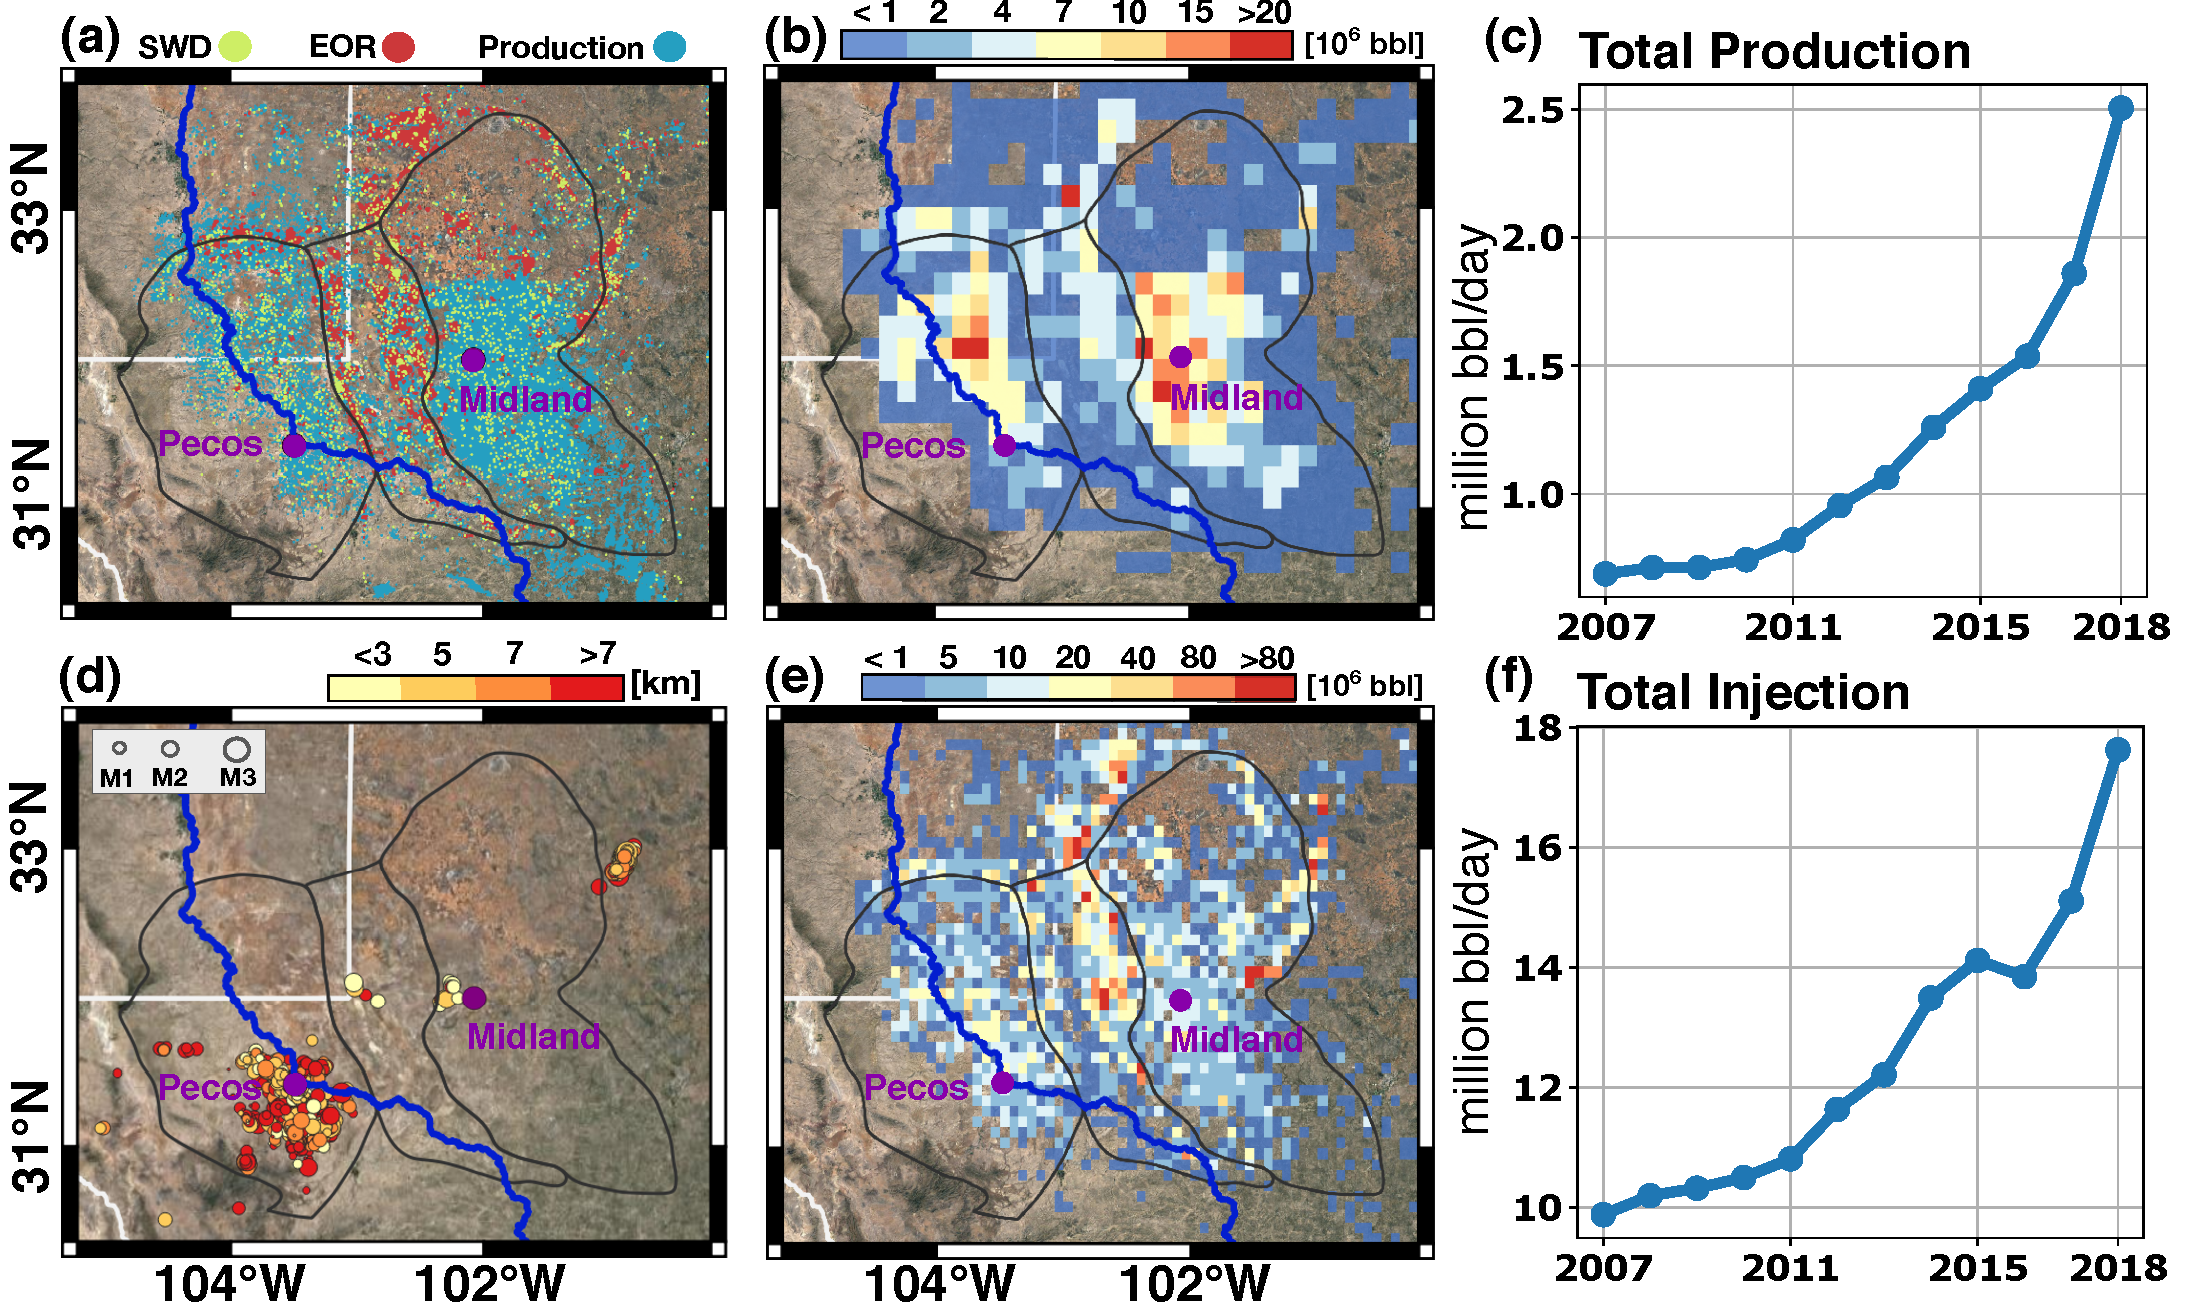
\includegraphics[width=0.99\linewidth]{paper1-permian/figures/supplement/figureS1-cisr-data.pdf}
	\caption[Shale development and induced seismicity in the Permian Basin.]{Shale development and induced seismicity in the Permian Basin. 
		(a) Locations of oil production, enhanced oil recovery (EOR), and saltwater disposal (SWD) wells active in 2017. (b) Annual oil production volume on a 10-mile grid in 2017. (c) Permian region oil production rate as reported by the Texas Railroad Commission. (d) Locations of earthquake hypocenters detected by TexNet in 2017. The color and size of a circle indicates the estimated earthquake depth and magnitude. (e) Annual injection volume (including both SWD and EOR wells) on a 5-mile grid. (f) Permian region injection rate (including both SWD and EOR wells) as reported by the Texas Railroad Commission.
	}
	\label{fig:Permian}
\end{figure*}


Understanding the nature and causes of earthquakes and how they are linked to certain production and disposal wells requires extensive knowledge of the subsurface. InSAR surface deformation measurements allow us to estimate the distribution of fault slip at depth and infer the associated seismic risk \citep{Segall2010, huang2017fault}. Furthermore, measurements of reservoir inflation due to wastewater injection allows operators to assess pressure build-up in disposal aquifers and the associated triggered seismicity risk. It is also worth noting that oil recovery in shale wells is notoriously low \citep{clark2009determination}, and the performance of these wells varies significantly. InSAR can be employed to map subsurface fluid depletion and pressurization. These surface deformation observations, when coupled with reservoir compaction inversion modeling, can be used to assess the areal effectiveness of oil and gas extraction operations \citep{Du2001, Vasco2005}. 
mechanically layered earth as a homogeneous half space, even though the stiffness increases with depth \citep{Du1992}. 




\chapter{InSAR Background}
\label{chap3}


\section{SAR Basics}
\label{chap3-sar}

\subsection{SAR Constellations}

- Make a figure with historial sar mission, and include private sector companies as well

\url{https://digitalcommons.usu.edu/cgi/viewcontent.cgi?article=5092&context=smallsat}

\url{https://www.newspace.im/ }

\url{https://www.newspace.im/constellations/iceye}


- There may be more SAR satellites launched in the next 5 years than cumulatively before this



The advantages long wavelengths offer in terms of penetration come with compensating drawbacks. The resolution a sensor depends on the wavelength and on the size of its aperture—the mirror or lens in the case of a camera or a telescope, the antenna in a radar. If you lengthen the wavelength, you increase the size of the aperture you need in order to achieve a given resolution. To produce detailed images with radar requires a very large aperture indeed—far larger than anything a single spacecraft can offer.

> Synthetic-aperture radar (SAR) provides a way round that problem. Satellites move at quite a clip—typically, in low orbit, around 25,000kph. By taking all the echoes a radar satellite gets from a given target as it passes over it—and processing them into a single image, SAR produces a result as precise as if it had been made using a single aperture as wide across as the distance the satellite travelled while gathering the data—tens of hundreds of kilometres (see diagram).

\section{InSAR Principles}

\section{InSAR Time Series}

stacking for avg rate

SBAS linear system. doesn't need to be short baseline. just a way to solve for the phase at each date

Phase linking approaches solve for this using an eptimization on each pixels time-covariance matrix.

\subsection{Uncertainty}

Several ways for uncertainty.

jackknife (maybe look into the NSBAS/GIANT time series way they do it....). prob an underestimate, since this is *precision* of the estimator. often it's jsut precision of the noise+deformation phase. but we really want the defo phase.

other is least squares propagation of covariance. difficult to calibrate without good atmo noise estimate, can underestimate/overestimate.

one problem with daily time series: often uncertainty is a single number. but each day's atmo noise can vary by 10-20x.

Even with temporal smoothing (example pic of that super storm cell), there can be many days with "blobs" of atmospheric noise which exceed real deformation.

Chapter (2nd paper) will discus a third novel way using computer vision.


Bootstrap:

From "practictioners guide":
A natural question for the practitioner is to ask  “ Why bootstrap in the linear regression case? Isn ’ t least - squares a well - established approach that  has  served  us  well  in  countless  applications? ”   The  answer  is  that  for  many  problems, least - squares regression has served us well and is always useful as  a first approach but is problematic when the residuals have heavy - tailed distributions or if even just a few outliers are present.



\section{Tropospheric Noise}


Tropospheric noise in InSAR consists of a stratified component, which correlates with topography \citep{Doin2009CorrectionsStratifiedTropospheric}, and a turbulent component that is random at time scales longer than a day \citep{Emardson2003NeutralAtmosphericDelay, Onn2006ModelingWaterVapor}. Previous studies have made advances in correcting for the stratified component using global atmospheric models \citep{Doin2009CorrectionsStratifiedTropospheric, Jolivet2014ImprovingInsarGeodesy, Cao2021AdvancedInsarTropospheric}, GPS zenith delay measurements \citep{Onn2006ModelingWaterVapor}, external measurements from sensors such as the Moderate Resolution Imaging Spectroradiometer (MODIS) \citep{Li2005InterferometricSyntheticAperture, Barnhart2013CharacterizingEstimatingNoise} or the Medium Resolution Imaging Spectrometer (MERIS)  \citep{Ding2008AtmosphericEffectsInsar}, as well as empirical methods using regressions on InSAR phase and elevation \citep{Zebker2021AccuracyModelFree, Murray2021ClusterBasedEmpirical}.

Early efforts to correct or mitigate the turbulent atmospheric noise used a combination of high pass temporal filtering and low pass spatial filtering \citep{Ferretti2001PermanentScatterersSar, Berardino2002NewAlgorithmSurface}.
%- but as \citep{Liu2012SatelliteRadarInterferometry} notes, gaps in the acquistion, or strong non-Gaussianity from, e.g., severe thunderstorms, break the assumptions of equal variance among APS dates that these filters require.
Several research efforts have attempted to produce estimates of the atmospheric phase delay for each SAR acquisition directly from a time series of interferograms. \citep{Liu2012SatelliteRadarInterferometry} formulated the problem as a linear system using a network of small baseline interferograms. Since the problem of estimating both surface deformation and atmospheric delay is an ill-posed problem given only differential InSAR measurements, the authors assumed zero or known deformation of the study region, and they constrained the estimated troposphere to have zero mean. In an attempt to denoise time series of surface deformation, \citep{Tymofyeyeva2015MitigationAtmosphericPhase} averaged sets of redundant interferograms containing a common reference date, with an assumption of linear or slowly-varying deformation, and subtracted the estimated troposphere.

%  \citep{Havazli2021DetectionThresholdEstimates} almost does what i'm doing (with some type of stratified atmo too), it's just a random multiplier, and it looks like it was almost all simulation
An alternative approach to correcting for the tropospheric turbulence is to treat it as a stochastic noise source in time series analysis \citep{Simons2007InterferometricSyntheticAperture, Agram2015NoiseModelInsar} and estimate its covariance matrix either through auxiliary data sources \citep{Barnhart2013CharacterizingEstimatingNoise, Parker2015SystematicAssessmentAtmospheric} or directly from InSAR data \citep{Lohman2005SomeThoughtsUse}. While these approaches provide a measure of uncertainty in the deformation solution, the uncertainties are given for each pixel (or each model parameter), rather than for each visible deformation feature.




\chapter{InSAR Reveals 80000}
\label{chap-4-GRL}

\section{Introduction}


The Permian Basin, stretching from eastern New Mexico and covering most of West Texas, has become the United States' largest producer of oil and gas over the past decade due to advances in shale recovery technologies. Injection or withdrawal of fluids from the subsurface can induce earthquakes along existing faults \citep{Ellsworth2013InjectionInducedEarthquakes, Simpson1988TwoTypesReservoir}, and an increased rate of low magnitude earthquakes have been observed along with the increase in hydrocarbon production in West Texas \citep{Frohlich2016HistoricalReviewInduced, Atkinson2016HydraulicFracturingSeismicity, Frohlich2019OnsetCauseIncreased, Lomax2019ImprovingAbsoluteEarthquake, Savvaidis2020InducedSeismicityDelaware, Skoumal2020InducedSeismicityDelaware}. While petroleum production and wastewater injection volumes have been rising throughout the basin, the recently cataloged earthquakes are spatially clustered. One significant cluster is near Pecos, TX, where increased seismic activity began in 2009 and climbed to more than 2000 earthquakes in 2017 \citep{Frohlich2019OnsetCauseIncreased}. To better understand the causes of these earthquakes and to assess the likelihood of infrastructure damage and safety concerns, the State of Texas funded the Texas Seismological Network (TexNet) to record earthquakes down to M2.0 across the state since 2017 \citep{Savvaidis2019TexnetStatewideSeismological}. TexNet seismic data will be most meaningful when combined with knowledge of the subsurface \citep{Council2013InducedSeismicityPotential, TheAcademyofMedicine2017EnvironmentalCommunityImpacts}; however, measuring the subsurface at a basin-scale is both expensive and technically challenging.

Interferometric Synthetic Aperture Radar (InSAR) has been routinely used for mapping surface deformation over wide areas with millimeter-to-centimeter accuracy \citep{Massonnet1993DisplacementFieldLanders, Buergmann2000SyntheticApertureRadar}.  These surface deformation measurements can be used to derive information about Earth's subsurface, estimate the distribution of fault slip, and infer associated seismic risk \citep{Segall2010EarthquakeVolcanoDeformation, Elliott2016RoleSpaceBased, Huang2017FaultGeometryInversion}. Within Texas, \cite{Shirzaei2016SurfaceUpliftTime} reported indications of surface uplift due to wastewater injection near a 2012 M4.8 earthquake, though limited validation for the ALOS data was available at this site near Timpson, TX \cite{Semple2017IncompleteInventorySuspected}. \cite{Kim2018AssociationLocalizedGeohazards} detected multiple deformation bowls within the Delaware Basin related to wastewater injection, $CO_2$ injection, and hydrocarbon production using Sentinel-1 InSAR data. \cite{Zheng2019WastewaterLeakageWest} incorporated InSAR-derived surface deformation data into a poroelastic model to analyze the geomechanical processes near an uplift signal in northern West Texas. They discovered that the observed surface deformation was likely caused by injection well leakages, rather than pressure increases at the planned injection depth, and the leaks may have contributed to freshwater contamination. More recently, \cite{Deng2020SurfaceDeformationInduced} used ascending Sentinel-1 LOS measurements to infer pore pressure change and Coulomb failure stress change at three sites in the southern Delaware Basin. They suggested that certain groups of earthquakes are likely induced by fluid injection, but noted that local rock structure and media properties are key controls on the area's susceptibility to induced seismicity.

Previous InSAR studies demonstrated the use of InSAR surface deformation data for understanding causes of induced seismicity; however, these studies only focused on study areas $ \sim $ 60-by-60km or smaller, and basin-wide InSAR surface deformation data with detailed uncertainty quantification are needed for assessing the likelihood of induced seismicity risk. Since InSAR tropospheric noise variance increases with the distance away from the reference point \citep{Emardson2003NeutralAtmosphericDelay}, it is difficult to expand the InSAR spatial coverage to the entire Permian basin while retaining millimeter level accuracy. In this study, we show that the increasing quantity and quality of Sentinel-1 SAR data allows us to average thousands of interferograms and mitigate strong tropospheric noise. Additionally, we developed an outlier detection algorithm that removes InSAR measurements corrupted by severe tropospheric noise (e.g. storms and heat waves) and reduces InSAR measurement uncertainty by another factor of 2, down to 1-3 mm/year across the basin. Our results were validated by independent GPS measurements recorded at 13 permanent ground stations. The InSAR-observed subsidence patterns over the Pecos area can be modeled as dip-slip over multiple normal faults and discretized cylindrical reservoir compaction. Our InSAR deformation maps are now available through the Center for Integrated Seismicity Research (CISR) for the broader scientific community. This dataset, when combined with physics-based reservoir and fault modeling, can produce insights into the causes of induced seismicity. Furthermore, these surface deformation data products can be used to assess the areal effectiveness of the oil and gas production, a measure for estimating which regions of a reservoir are being depleted most quickly. InSAR techniques now provide a low-cost method to assist oil and gas operations and risk management at a basin-scale.

\section{Methods}
\subsection{InSAR data processing strategy}
\label{sec:InSARprocessing}
Using a geocoded SLC processor \citep{Zheng2017PhaseCorrectionSingle, Zebker2017UserFriendlyInsar}, we processed 91 ascending (path 78, frames 94-104) and 82 descending (path 85, frames 483-493) Sentinel-1 scenes acquired between Nov. 2014 and Jan. 2019 (Figure \ref{fig:paper1-study-area}). We generated more than 7000 interferograms with 120 meter pixel spacing and a maximum temporal baseline of 800 days. No spatial baseline threshold was imposed in the interferogram formation. Because few decorrelation artifacts were presented, we were able to unwrap all interferograms without additional spatial filtering using the Statistical-cost, Network-flow Algorithm for Phase Unwrapping (SNAPHU) \citep{Chen2001TwoDimensionalPhase}. We removed long-wavelength phase ramps, possibly due to residual orbit errors or long-wavelength tropospheric noise, using a planar phase model. Comparable interferograms can be generated using other processors such as the InSAR Scientific Computing Environment (ISCE) \citep{Rosen2012InsarScientificComputing}. 


\begin{figure}[hbt!]
	\centering
	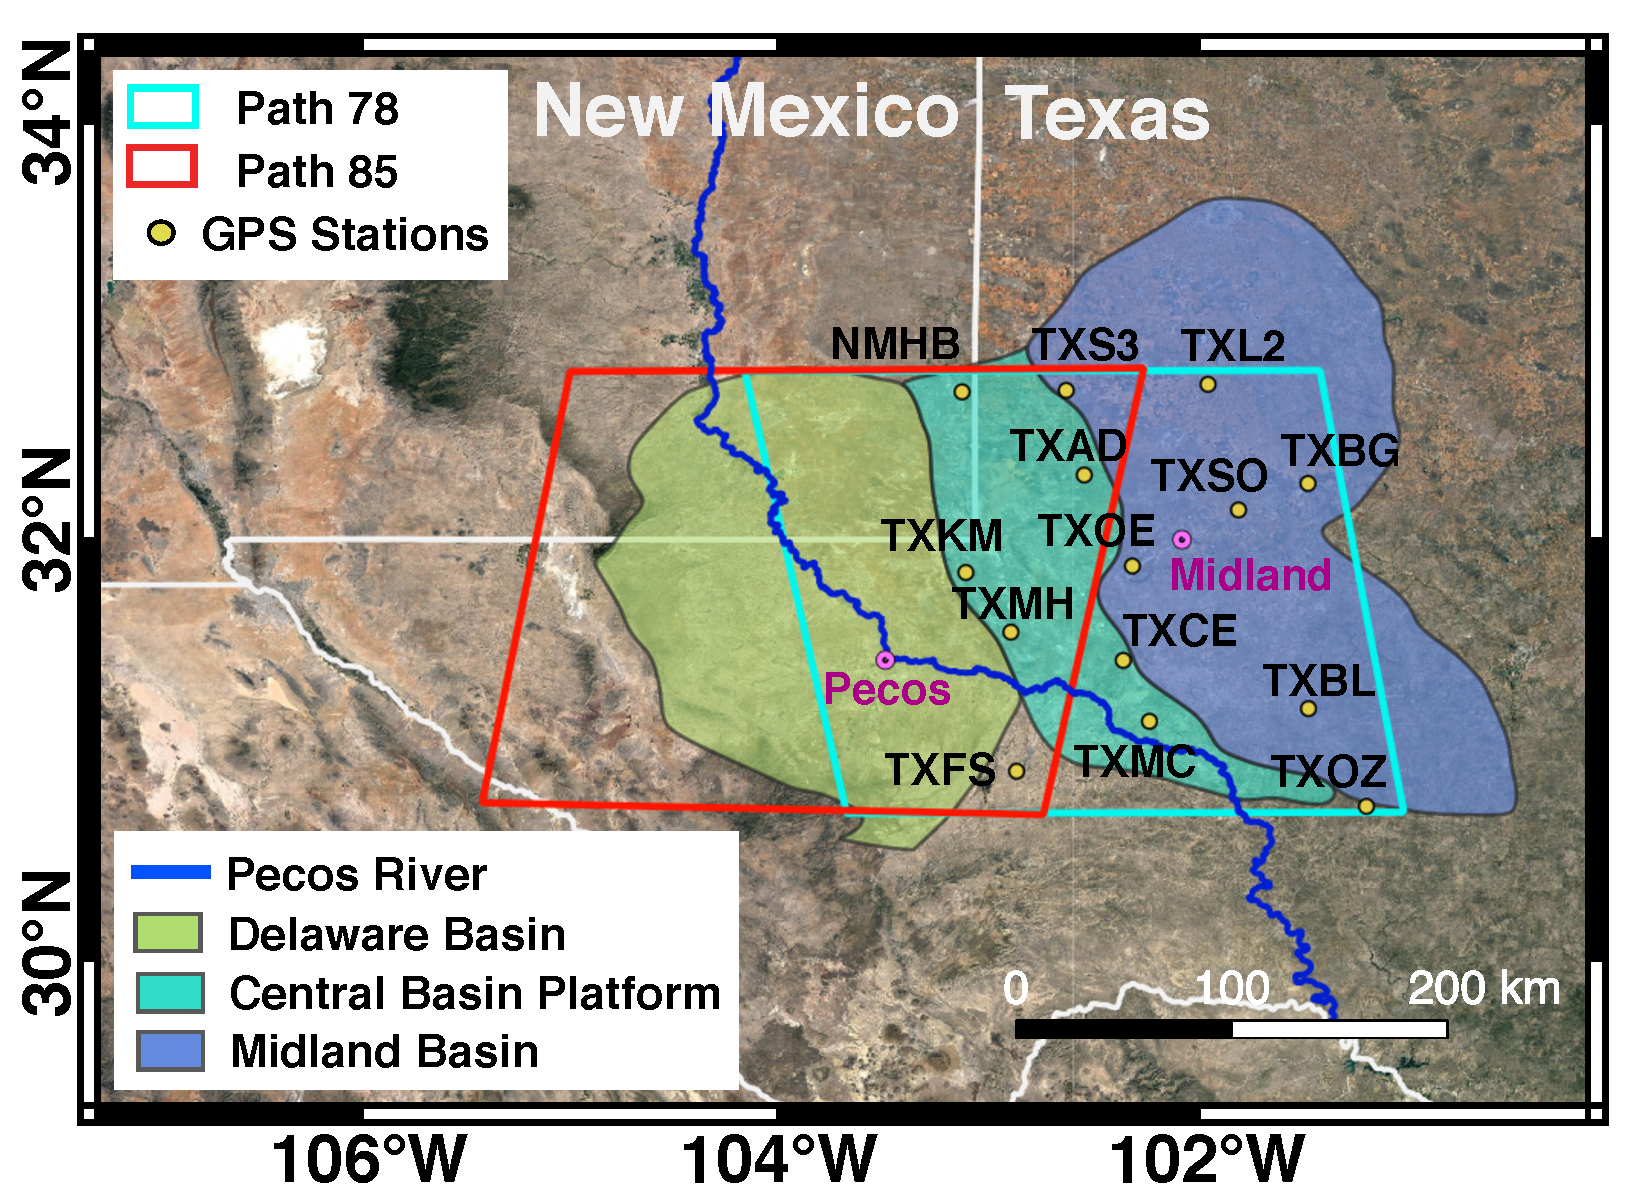
\includegraphics[width=0.9\linewidth]{paper1-permian/figures/figure1-study-area.pdf}
	\caption[GPS and InSAR data coverage over the Permian Basin.]{GPS and InSAR data coverage over the Permian Basin. Yellow dots indicate GPS permanent stations. Teal and red boxes indicate ascending path 78 and descending path 85 paths of Sentinel 1 InSAR coverage, respectively. Each path contains over 80 SAR acquisitions, leading to over 3500 interferograms per path at 120 m pixel spacing.}
	\label{fig:paper1-study-area}
\end{figure}


The coverage of GPS permanent stations in West Texas is sparse, and there are 14 permanent GPS stations (Figure \ref{fig:paper1-study-area}) that recorded daily east, north, and up (ENU) surface deformation measurements \citep{Blewitt2018HarnessingGpsData}. After removing the common tectonic motion, all GPS stations showed little surface deformation (0-3 mm/year) between Nov. 2014 and Jan. 2019. We chose the GPS station TXKM as the reference point for both ascending and descending InSAR data, and we used the remaining 13 stations as controls to assess InSAR measurement uncertainty as described in Section \ref{sec:errors}.

\subsection{Solutions for cumulative surface deformation over time}
\label{sec:stacking}
An interferogram measures surface deformation that occurred between the two SAR acquisition times along the radar line-of-sight (LOS) direction \citep{Hanssen2001RadarInterferometryData}. We employed a stacking approach \citep{Sandwell1998PhaseGradientApproach} to calculate the average LOS velocity $v_{avg}$ of each ground pixel over a time period of interest $T$ as:
\begin{equation}
	v_{avg} = \frac{\sum_{i \in G} d_i}{\sum_{i \in G} t_i}
	\label{eq:stacking}
\end{equation}
where $G$ is a subset of interferograms that were formed using two SAR scenes acquired within the time period $T$. The LOS measurement (in cm) and the temporal baseline of the $i^{th}$ interferogram in $G$ are written as $d_i$ and $ t_i $ respectively. Comparable LOS velocity estimates can be produced using the Small Baseline Subset (SBAS) approach \citep{Berardino2002NewAlgorithmSurface} with a constant velocity (linear deformation) model (TODO: \textit{Supporting Information S5}).

In this study, we solved for the average LOS velocities over three periods of interest: Nov. 2014 to Jan. 2017, Nov. 2014 to Jan. 2018, and Nov. 2014 to Jan. 2019. Over each period $T_j$, we computed the cumulative LOS surface deformation over this period as the product of $v_{avg,j}$ and $T_j$. We also solved for the vertical and eastward deformation in the region where path 78 and 85 overlap ( \textit{Supporting Information S2}). To account for the large variation in look angle within one Sentinel-1 Interferometric Wide (IW) swath image, we used the LOS unit vector at each pixel location (Figure S2) in the LOS decomposition.


\section{A comparison between stacking and InSAR time series methods}
\label{sec:method-compare}
If data error treatments and deformation model assumptions are valid, we can derive meaningful and comparable deformation solutions using different InSAR time series analysis methods. To investigate how InSAR measurement noise influences the LOS deformation solutions, we compared the results derived from (1) the stacking method, (2) a Small BAseline Subset (SBAS) linear deformation (constant velocity) model with $L_1$ and $L_2$-norm penalty functions, and (3) unregularized and regularized SBAS deformation time series. 

For the remainder of this section, we assume there are $M$ small-baseline interferograms that were generated from $N$ SAR scenes acquired over a period of interest. The stacking method from \cite{Sandwell1998PhaseGradientApproach} that we employed in this study solves for the average velocity over the study period. Similarly, the SBAS linear deformation model solves for the average velocity $ v_{avg} $ over this period at each pixel of interest as \citep{Berardino2002NewAlgorithmSurface}:
\begin{equation}
	\arg \min_{v_{avg}} \norm{ \bm{BP} v_{avg} - \bm{d}   }_p
	\label{eq:sbas-linear}
\end{equation}
where $ \bm{B }$ is the $ M \times (N-1) $ SBAS matrix, $ \bm{P}$ is an $ (N-1) \times 1 $ vector of ones, $ \bm{d} $ is the $ M \times 1 $ vector of LOS measurements (in cm) at this pixel, and $ p \in \{1, 2\} $ is the norm used to penalize the data misfit. The $L_2$ linear deformation solution is comparable to the stacking solution (with an assumption of a constant velocity), and the $L_1$ solution is typically less sensitive to measurement outliers than the $L_2$ solution.

The LOS surface velocities between adjacent SAR acquisitions $ \bm{v} = \left[v_1 , \ldots , v_{N-1} \right]^T $ can be solved as:
\begin{equation}
	\arg \min_{\bm{v} } \norm{ \bm{Bv} - \bm{d}   }^2_2 + \alpha \norm{ \bm{Dv} }^2_2  \label{eq:sbas}
\end{equation}
where $ \bm{D} $ is a $ (N-2) \times (N-1) $ matrix, with $1$ on the main diagonal and $-1$ on the superdiagonal, which approximates the first-order differentiation operator. The first term penalizes the data misfit, the second term is a temporal smoothness constraint, and $ \alpha \in \Bbb{R} $ is the weight between the two terms. When $ \alpha = 0 $, the solution is the unregularized SBAS deformation time series. An additional integration of $\mathbf{v}$ over time yields the LOS deformation time series.

Little surface deformation occurred between Nov. 2014 and Jan. 2019 at the 13 GPS permanent GPS stations. At each GPS location, we projected the GPS time series to the radar line-of-sight (LOS), and we used the GPS-inferred average LOS velocity (0-3 mm/year) as ground truth. Table \ref{tab:compare-errors} shows the root mean square (RMS) and the worst-case absolute differences between InSAR and GPS inferred average LOS velocities between Nov. 2014 and Jan. 2018 as derived from the four InSAR time series methods. We found that InSAR tropospheric noise has a strong influence on all the surface deformation solutions before removing the measurement outliers. As an example, Figure \ref{fig:compare} (a) shows the ascending LOS solutions between Nov. 2014 and Jan. 2018 at the GPS station TXSO before removing InSAR measurement outliers. The random tropospheric noise creates up to $\sim$6 cm of error in the unregularized SBAS surface deformation time series. This error can be reduced by increasing $ \alpha$ in Equation \eqref{eq:sbas}. As $\alpha$ increases, the LOS deformation time series converge to the $L_2$ linear deformation (constant velocity) solution. However, there are visible cm-level tropospheric artifacts in the cumulative deformation solutions by using either $L_1$ or $L_2$ linear deformation models (e.g. Figure 2 (d) in the main text). 

After removing InSAR outlier measurements associated with extreme local weather events as described in Section 2.3 (main text), all SBAS time series methods produce more accurate and consistent deformation trends (Figure \ref{fig:compare} (b)). The unregularized SBAS time series still contain up to $\sim$3 cm of tropospheric noise, which leads to long-wavelength artifacts in the basin-wide deformation maps. The $ L_1 $ and $ L_2 $ linear deformation solutions show close agreement ($<$ 2 mm difference) at all GPS stations. Since both methods suggest a deformation trend consistent with the stacking approach, we chose the simple stacking method as the final processing strategy for estimating cumulative surface deformation in the Permian Basin.

\begin{figure}
	\centering
	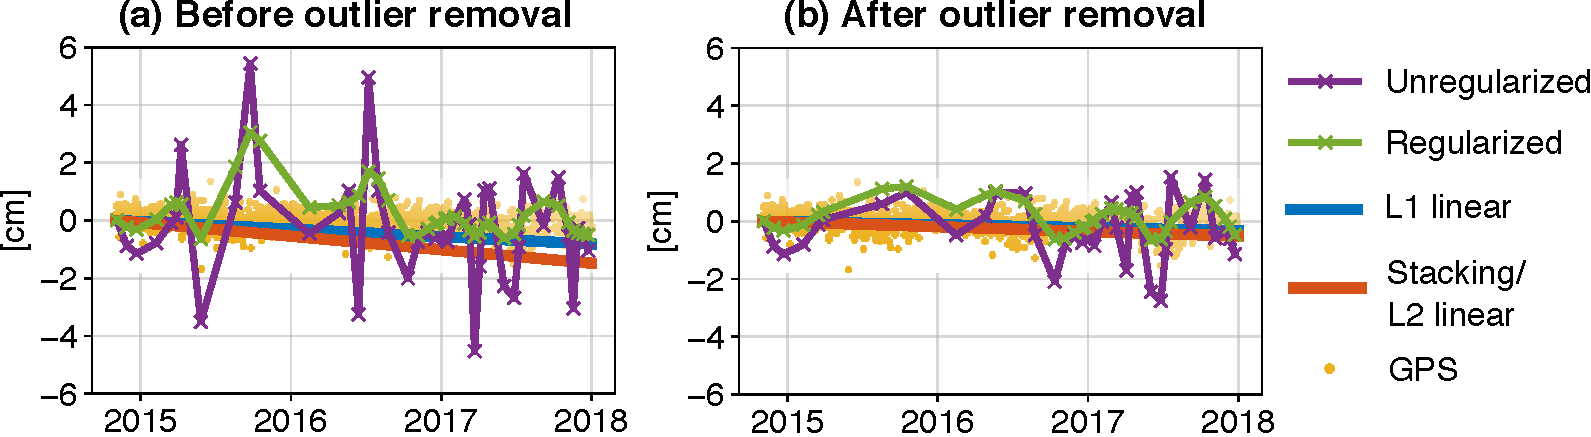
\includegraphics[width=\textwidth]{paper1-permian/figures/supplement/figureS5-compare-insar-2panel.pdf}
	\caption[Comparisons of InSAR SBAS solutions]{Comparisons of InSAR unregularized SBAS time series (purple), regularized SBAS time series (green), linear deformation trend estimated by minimizing the $L_1$-norm of the residuals (blue), and the $L_2$-norm of the residuals/ stacking approach (red)  (a) before and (b) after removing LOS measurement outliers. ENU GPS data from station TXSO has been projected onto the radar LOS (orange dots).}
	\label{fig:compare}
\end{figure}

\subsection{Errors in InSAR surface deformation estimates}
\label{sec:errors} 
The phase of an interferogram can be written as \citep{Zebker1992DecorrelationInterferometricRadar, Zebker1994AccuracyTopographicMaps, Zebker1997AtmosphericEffectsInterferometric}
\begin{equation}
	\Delta \phi = \frac{4 \pi}{\lambda} \Delta d_{LOS} +  \Delta \phi_{orb} + \Delta \phi_{decor} + \Delta \phi_{unwrap}  + \Delta \phi_{dem} + \Delta \phi_{iono} + \Delta \phi_{tropo}  + \Delta \phi_{n}
\end{equation}
where $ \lambda $ is the radar wavelength and $ \Delta d_{LOS} $ is the surface deformation along the radar LOS direction. The noise terms include orbital errors, phase decorrelation, unwrapping errors, DEM inaccuracies, ionospheric and tropospheric artifacts, and other residual noise terms that are typically an order of magnitude smaller than the error terms listed here. Following the processing strategy outlined in Section \ref{sec:InSARprocessing}, $\Delta \phi_{orb}$, $\Delta \phi_{decor}$, and $\Delta \phi_{unwrap}$ were either removed or negligible in our dataset. Because the relatively flat Permian Basin is located in the middle latitudes, $\Delta \phi_{dem}$ and $\Delta \phi_{iono}$ are not substantial \citep{Fattahi2013DemErrorCorrection, Liang2019IonosphericCorrectionInsar}. For the reminder of this section, we focused on evaluating and mitigating the impact of tropospheric noise on the West Texas Sentinel-1 data.


%
%\subsection{The impact of the stratified component of tropospheric noise}
%\label{sec:noise-quant}


Tropospheric noise $\Delta \phi_{tropo}$ consists of a stratified component that correlates with topography \citep{Doin2009CorrectionsStratifiedTropospheric} and a turbulent component that is random at time scales longer than one day \citep{Emardson2003NeutralAtmosphericDelay}. We checked for a stratified tropospheric noise component using the Generic Atmospheric Correction Online Service (GACOS), and we found that the stratified tropospheric errors in our Sentinel-1 data are minimal (Figure \ref{fig:GACOS}).  GACOS is an iterative tropospheric decomposition model that integrates global weather models and available GPS zenith delay measurements for estimating tropospheric noise in InSAR data \citep{Yu2018InterferometricSyntheticAperture}. Due to the limited spatial and temporal resolution of weather models and GPS data, GACOS is more effective in removing the stratified tropospheric noise \citep{Doin2009CorrectionsStratifiedTropospheric} than the random turbulent tropospheric noise \citep{Emardson2003NeutralAtmosphericDelay}. We found that GACOS does not produce substantial corrections in most Sentinel-1 West Texas interferograms (e.g. Figure \ref{fig:GACOS} (a)-(c)). This is because the oil-producing region of the Permian Basin is relatively flat, and we observed little correlation between InSAR LOS measurements and the Digital Elevation Model (DEM) data (e.g. Figure \ref{fig:GACOS} (d)). We thus concluded that the stratified tropospheric noise was minimal in our study region.


\begin{figure}
	\centering
	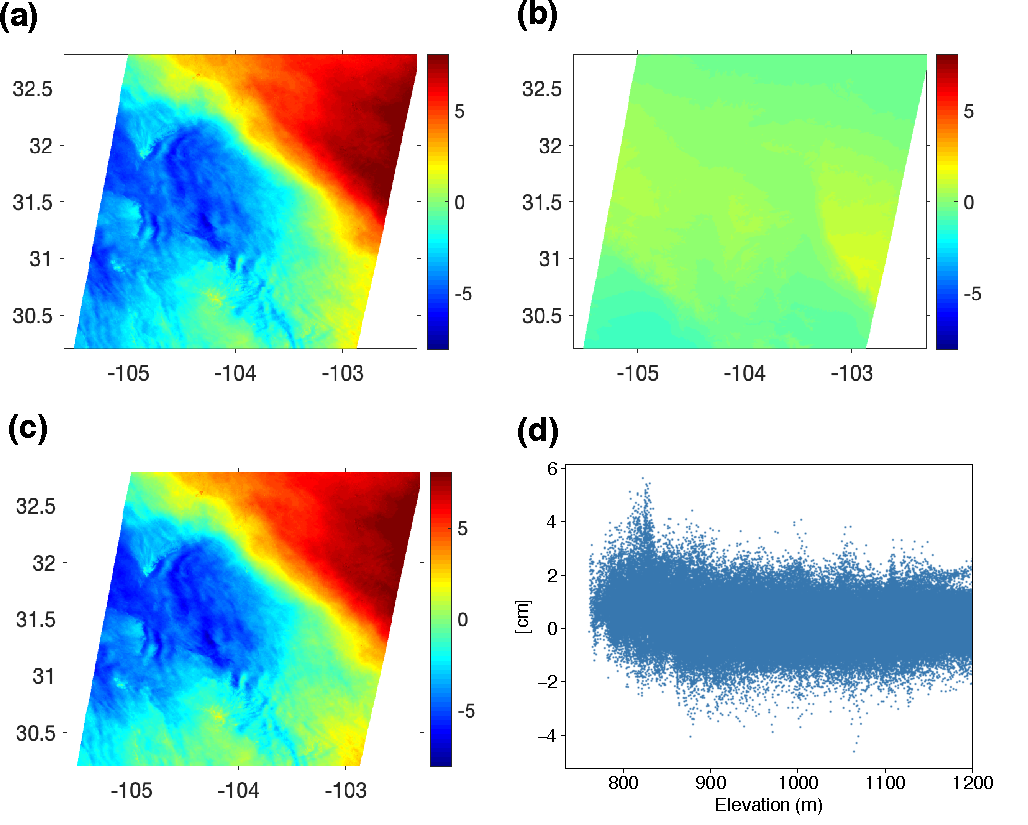
\includegraphics[width=\textwidth]{paper1-permian/figures/supplement/figureS4-gacos.pdf}		
	\caption[GACOS tropospheric corrections]{(a) LOS measurements (in cm) of a descending interferogram (20150127-20150220) before the GACOS correction. (b) GACOS tropospheric correction (in cm) for the 20150127-20150220 interferogram \citep{Yu2018InterferometricSyntheticAperture}. (c) LOS measurements (in cm) of a descending interferogram (20150127 - 20150220) after the GACOS correction. (d) LOS measurements (in cm) of the 20150127-20150220 interferogram vs. the Digital Elevation Model (DEM).}
	\label{fig:GACOS}
\end{figure}



We further examined interferograms at the 13 control locations. For example, LOS measurements of the ascending interferograms at pixels near the GPS station TXMC show a near zero median (-4 mm) and a standard deviation of 3.2 cm (Figure \ref{fig:outliers} (a)). Due to the absence of substantial deformation signal at this station, the standard deviation of the LOS distribution is a measure of turbulent tropospheric noise.  We found that the median LOS turbulent error is close to zero (no systematic noise bias) at all GPS control stations. The standard deviation of the turbulent noise increases as the square root of the distance from the InSAR reference point (Figure \ref{fig:outliers} (b)). Furthermore, we compared the LOS turbulent noise distribution observed at each GPS station to a normal distribution using a normal probability plot \citep{Filliben1975ProbabilityPlotCorrelation}. We discovered that non-Gaussian tails (outliers) are present (e.g. Figure \ref{fig:outliers}(c)) as a result of severe tropospheric noise (e.g. storms or heat waves). Identifying and removing these InSAR measurement outliers is crucial for achieving millimeter level accuracy. 




\begin{figure}[hbt!]
	\centering
	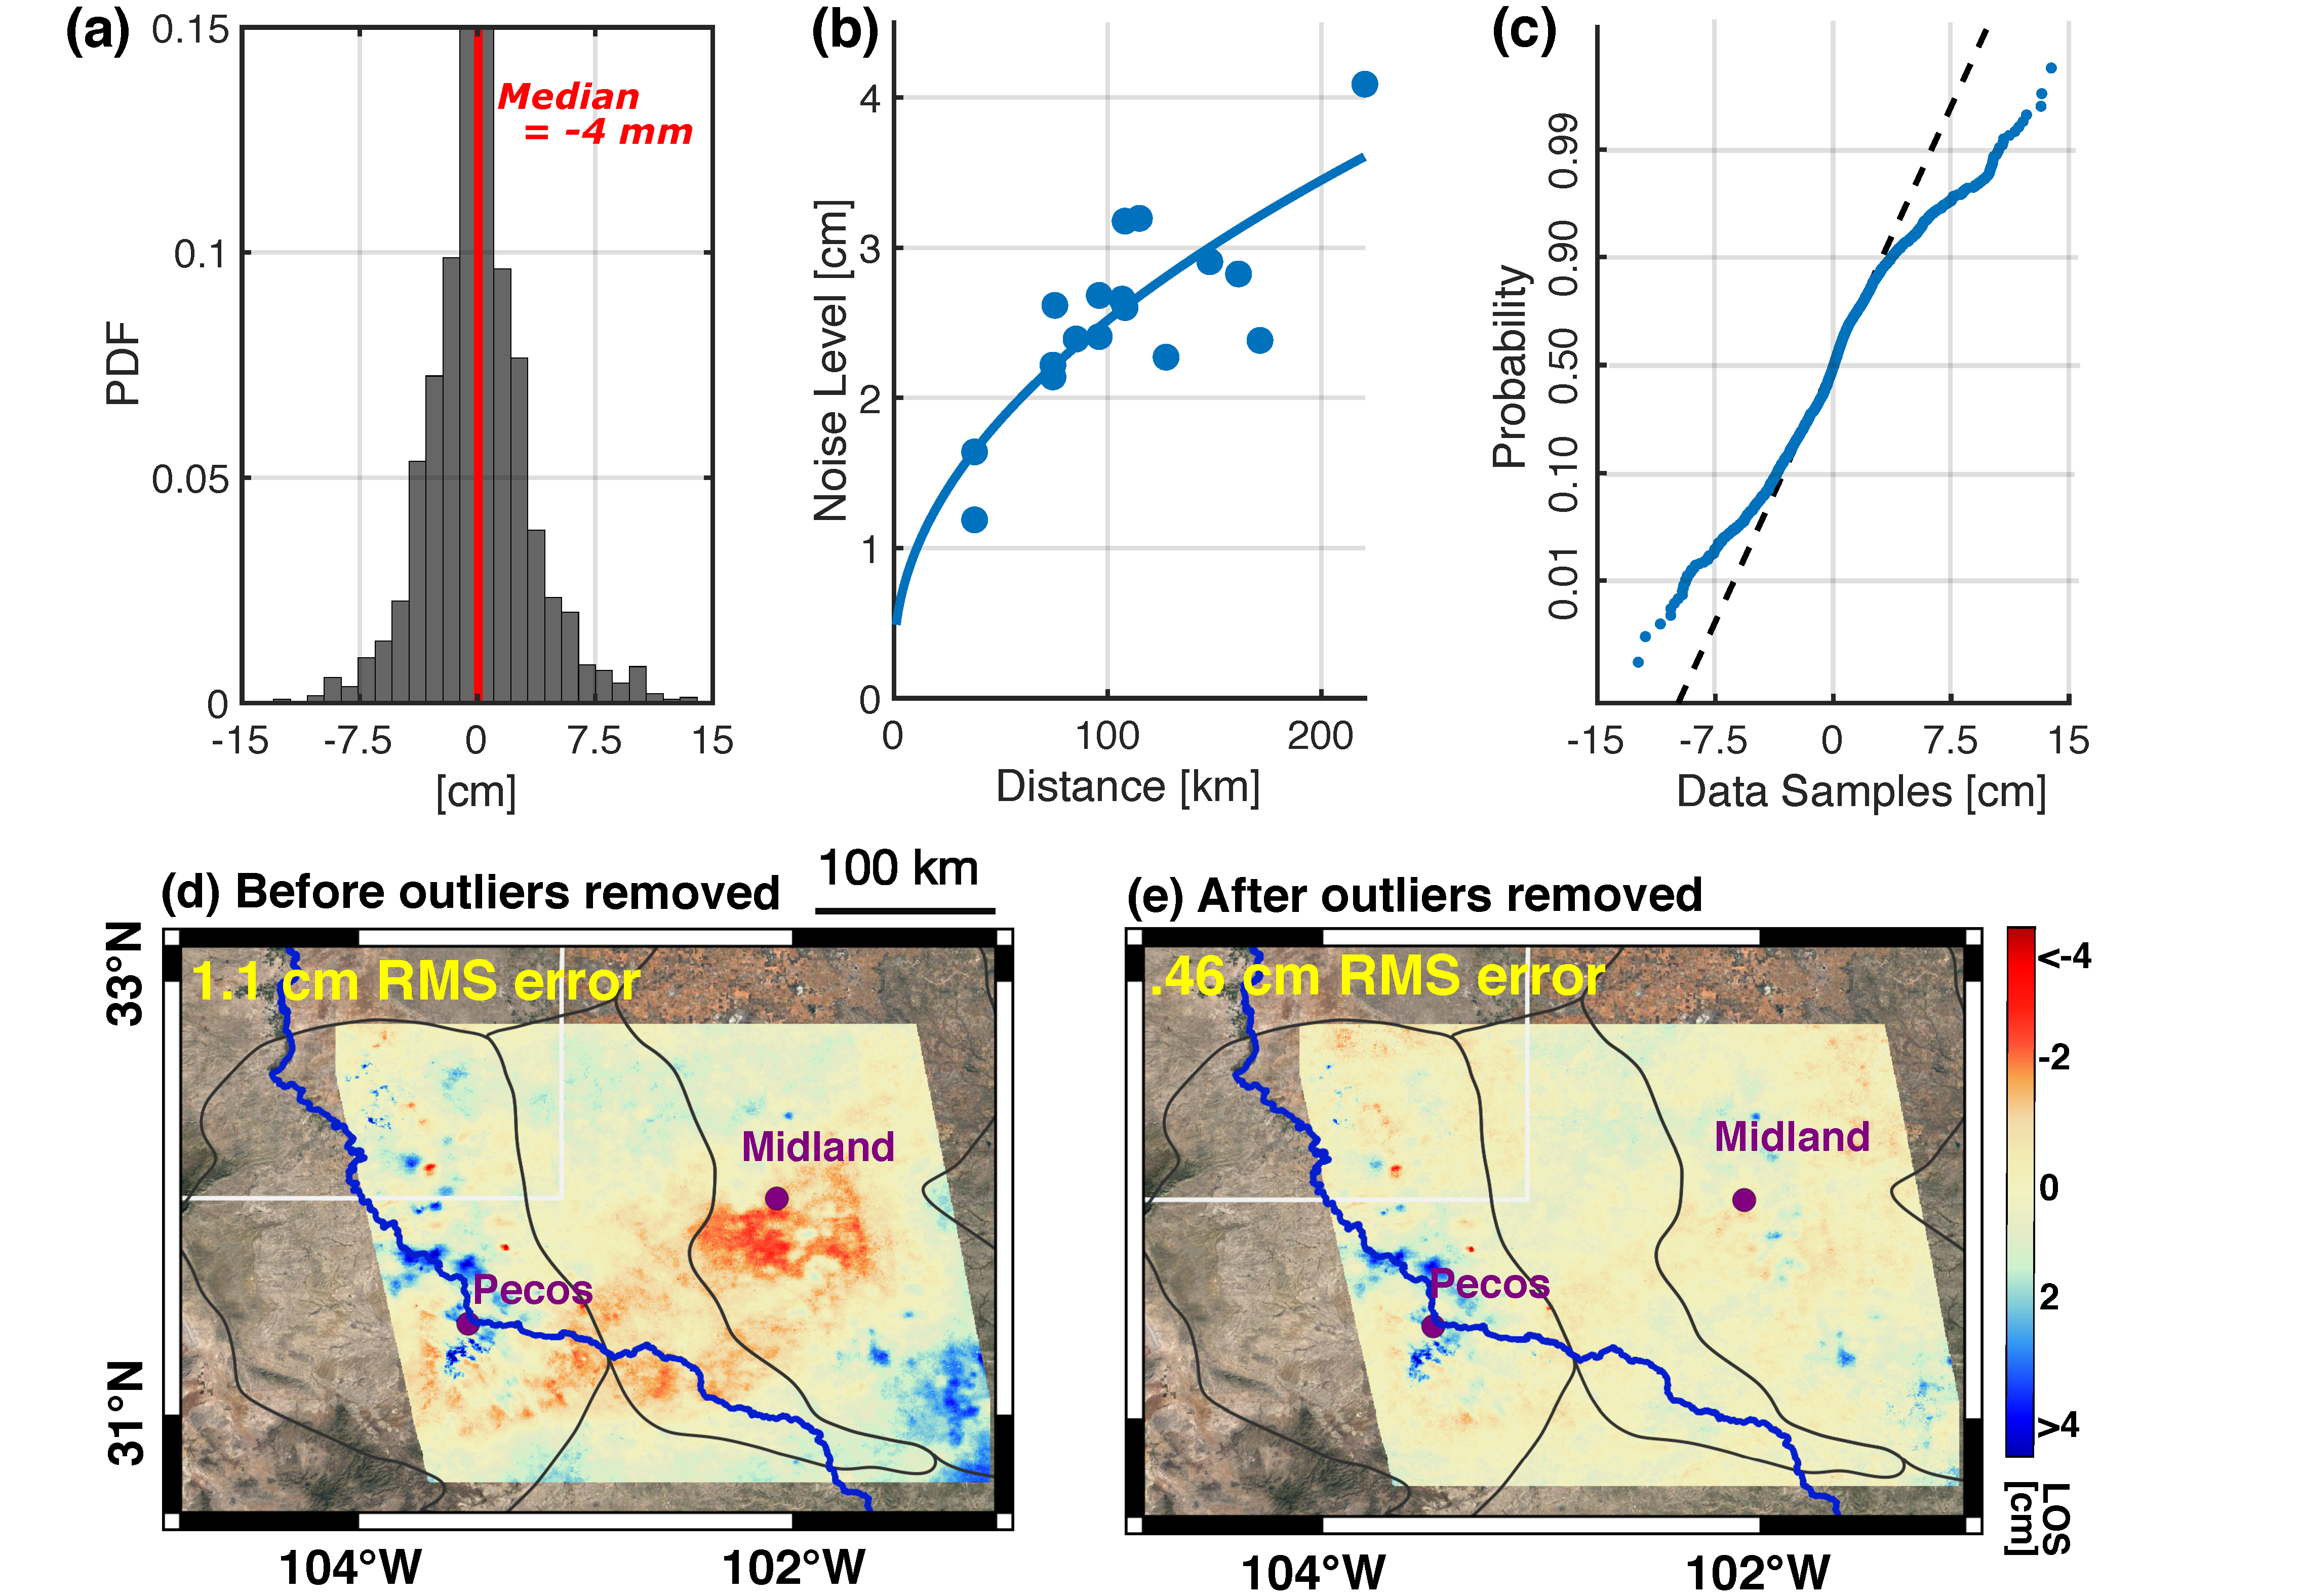
\includegraphics[width=0.95\linewidth]{paper1-permian/figures/figure2-outlier-removal-5panel.pdf}
	\caption[Noise measurement and tropospheric outlier removal comparison]{(a) LOS measurements (in cm) of all ascending interferograms at the GPS station TXMC. The distribution has a near zero median (-4 mm) and a standard deviation of 3.2 cm. Due to the absence of substantial deformation signals, the standard deviation of the distribution is a measure of LOS turbulent tropospheric noise. (b) The standard deviation of random tropospheric turbulent noise at 13 control locations (blue dots), which increases as the square root of the distance from the InSAR reference point (blue line). (c) A comparison between the tropospheric noise distribution at TXMC with a normal distribution. Dashed line connects the 1st and 3rd quartiles of the data. Troposphere noise following a normal distribution would match the dashed line, and non-Gaussian tails (we noted as outliers) are present. Cumulative ascending LOS deformation solutions (Nov. 2014 - Dec. 2017) (d) before and (e) after excluding InSAR outlier measurements. Note that 1.1 cm cumulative error over 3 years is equivalent to 3.5 mm/year RMS error in the velocity estimate.}
	\label{fig:outliers}
\end{figure}


Because severe tropospheric noise may only affect a portion of a SAR image, we identified InSAR measurement outliers at each pixel independently as follows. Given $N$ SAR acquisitions, there are up to $N-1$ InSAR LOS measurements at a pixel of interest that contain the common tropospheric noise of the $k^{th}$ SAR scene. We defined $u_{k,n}$ as the $n^{th}$ such LOS measurement, and $\bar{u}_k$ as:
\begin{equation}
	\bar{u}_k  = \frac{1}{N-1} \sum_{n=1}^{N-1} |u_{k,n}|  
\end{equation}
We labeled $u_{k,n}$ (for all $n$) as outlier measurements if $\bar{u}_k > \mathrm{median}(\mathbf{\bar{u}}) + 4 \sigma_{\mathrm{MAD}}$, where $\mathbf{\bar{u}}=[\bar{u}_1,...,\bar{u}_N]$, and $\sigma_{\mathrm{MAD}}=1.483 \cdot \mathrm{MAD}(\mathbf{\bar{u}})$. Here we employed a robust statistics measure, the median absolute deviation (MAD), for estimating the spread of data samples in the presence of outliers \cite{Hampel1974, Rousseeuw2011}. Given a vector $\mathbf{x}$ that contains $M$ data samples, $\mathrm{MAD}(\mathbf{x})$ is defined as:
\begin{equation}
	\mathrm{MAD}(\mathbf{x}) =  \underset{m = 1,\ldots M}{\mathrm{median}} \left( \bigr\lvert  x_m - \mathrm{median}(\mathbf{x})  \bigr\rvert \right)
\end{equation}
where $x_m$ is the $m^{th}$ data sample. 

To evaluate the performance of our InSAR processing strategy, we projected GPS data recorded at 13 control stations onto the LOS directions to use as ground truth. The differences between InSAR and GPS inferred average LOS velocities were used as a measure of the uncertainty in the InSAR surface deformation solutions (\textit{Supporting Information S4}). We found that stacking reduces the impact of random Gaussian turbulent noise by $ \sim \sqrt{N} $, where $ N $ is the number of SAR acquisitions. The outlier removal algorithm further reduces the uncertainty in the LOS velocity estimates by a factor of 2, down to 1-3 mm/year across the basin. For example, the average InSAR velocity along the ascending LOS direction between Nov. 2014 and Jan. 2018 shows a root mean square (RMS) error of 3.4 mm/year before the outlier removal, and 1.5 mm/year after the outlier removal. The presence of InSAR measurement outliers resulted in long-wavelength artifacts ($ \sim $100km and greater) in the cumulative deformation solutions (e.g. Figure \ref{fig:outliers} (d)), which were automatically mitigated through the pixel-based outlier removal algorithm (e.g. Figure \ref{fig:outliers} (e)). Additionally, we compared InSAR LOS deformation solutions as derived from (1) the stacking method, (2) a SBAS linear deformation model with $L_1$ and $L_2$-norm penalty functions, and (3) unregularized and regularized SBAS deformation time series (\textit{Supporting Information S5}). These InSAR time series algorithms can be implemented using software packages such as Generic InSAR Analysis Toolbox (GIAnT) \cite{agram2013new}, STAMPS \cite{hooper2012recent}, and LiCSBAS \cite{morishita2020licsbas}. Removing the detected outliers leads to more accurate and consistent surface deformation solutions in all three cases.


\subsection{InSAR LOS velocity estimation errors using the stacking method}
\label{sec:error-quant}
We used independently processed GPS east, north, and up GPS time series as ground truth to quantify errors in the InSAR stacking solutions before and after the outlier removal. There are 13 permanent GPS stations in the ascending SAR footprint. At each GPS location, we projected the GPS time series to the radar line-of-sight (LOS), and we computed the GPS-inferred average LOS velocity through a linear regression. Table \ref{tab:gps-error-78} shows the root mean square (RMS) and the worst-case absolute differences between InSAR and GPS inferred average LOS velocities over the three study periods. Similarly, there are 5 permanent GPS stations in the descending SAR footprint, and Table \ref{tab:gps-error-85} shows the uncertainty in the descending stacking solutions using these 5 GPS stations as control. Both Table \ref{tab:gps-error-78} and Table \ref{tab:gps-error-85} show that our outlier removal algorithm reduced the uncertainty in InSAR stacking solutions by a factor of $\sim$2, down to 1-2 mm/year across the basin. For a given period of interest $T_j$, the LOS velocity error $ E_{vel,j} $ propagates into the cumulative deformation error $ E_{c, j} $ as $ E_{c,j} = E_{vel,j} \cdot T_j $. 


\begin{table}
	\caption{InSAR ascending LOS velocity estimation errors (in mm/year) using the stacking method}
	\centering
	\begin{tabular}{|c|c|c|}
		\hline 
		& Before the outlier removal & After the outlier removal \\
		& (RMS / Worst) & (RMS / Worst) \\
		\hline
		Nov. 2014 - Jan. 2017 & 3.8 / 9.5         & 1.9 / 5.9       \\\hline
		Nov. 2014 - Jan. 2018 & 3.3 / 7.1         & 1.3 / 2.5       \\\hline
		Nov. 2014 - Jan. 2019 & 2.0 / 6.1         & 1.1 / 2.5       \\\hline                
	\end{tabular}
	\label{tab:gps-error-78}
\end{table}

\begin{table}
	\caption{InSAR descending LOS velocity estimation errors (in mm/year) using the stacking method}
	\begin{tabular}{|c|c|c|}
		\hline 
		& Before the outlier removal & After the outlier removal \\
		& (RMS / Worst) & (RMS / Worst) \\
		\hline 
		Nov. 2014 - Jan. 2017 & 7.8 / 13.8                            & 2.9 / 5.0                          \\\hline
		Nov. 2014 - Jan. 2018 & 3.7 / 7.5                             & 2.7 / 5.6                          \\\hline
		Nov. 2014 - Jan. 2019 & 1.6 / 2.8                             & 0.8 / 1.6  \\\hline     
	\end{tabular}
	\label{tab:gps-error-85}
\end{table}

\begin{table}
	\caption{Errors (in mm) in four SBAS ascending LOS deformation (Nov. 2014 - Jan. 2018) solutions}
	\centering
	\begin{tabular}{|c|c|c|}
		\hline 
		& Before the outlier removal & After the outlier removal \\
		& (RMS / Worst) & (RMS / Worst) \\
		\hline
		Unregularized &  22 / 99     &  14 / 43         \\\hline
		Regularized   &    14 / 63   &   10  / 27       \\\hline
		L1 linear deformation          &   7 / 11      & 4 / 8      \\\hline
		L2 linear deformation          &   10 / 22        & 4 / 8      \\\hline
	\end{tabular}
	\label{tab:compare-errors}
\end{table}



\section{Results and discussion}
\subsection{Surface deformation in the Permian Basin}
The Sentinel-1 cumulative LOS deformation solutions reveal numerous surface deformation features over the oil-producing region in the Permian Basin (Figure \ref{fig:insar-los}). From the ascending geometry, we observed no substantial deformation in the Central Basin Platform, where oil and gas are mostly produced from conventional reservoirs. In the Midland and Delaware Basins, we observed an accelerating surface deformation rate between Nov. 2014 and Jan. 2019, which coincides with the sharp rise of oil production from unconventional reservoirs in 2017 and 2018. For example, a 30 km$^2 $ area northwest of Pecos shows approximately 0.5 cm cumulative LOS deformation between Nov. 2014 and Jan. 2017, 1.5 cm between Nov. 2014 and Jan. 2018, and over 5.5 cm from Nov. 2014 to Jan. 2019. The greatest number of observable signals are present in 2018 when peak production occurred in the region. Similarly, from the descending geometry, we find no substantial deformation in the Central Basin Platform and an increasing rate of surface deformation in the Delaware Basin. 


\begin{figure*}[hbt!]
	\centering
	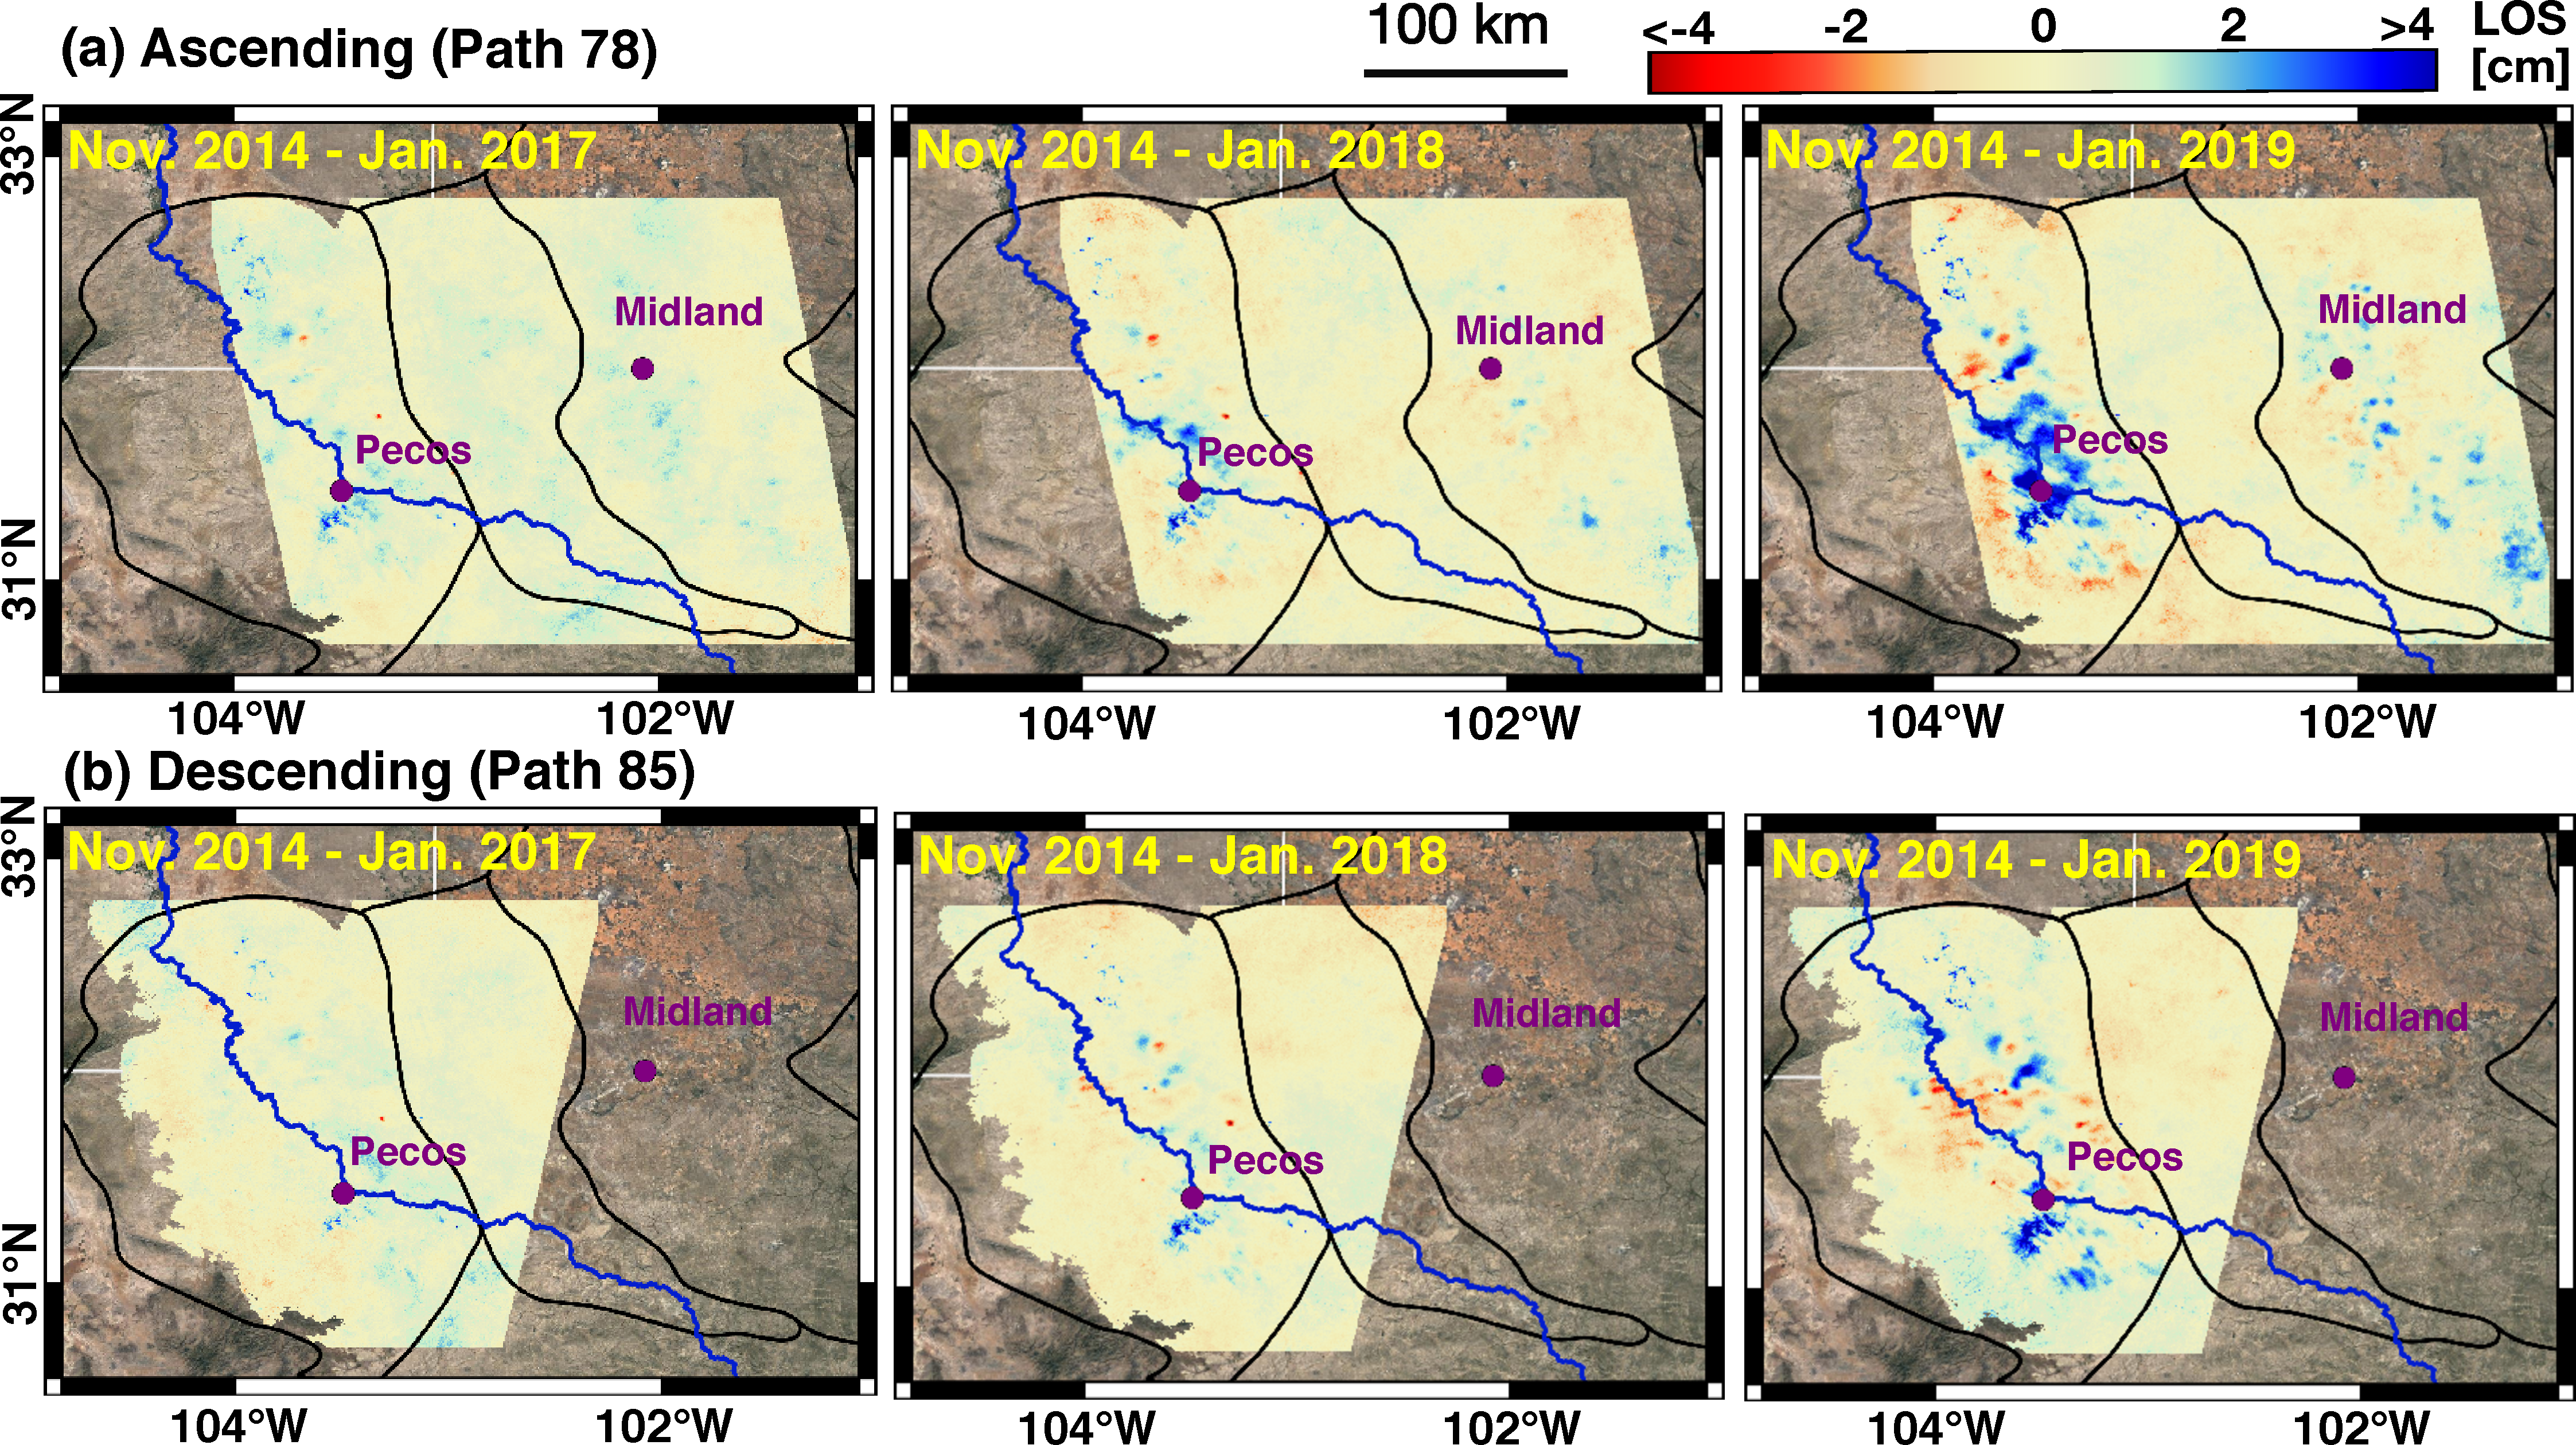
\includegraphics[width=.96\linewidth]{paper1-permian/figures/figure3-los-insar.pdf}
	\caption[Cumulative LOS deformation for path 78 and path 85]{Cumulative LOS deformation (Nov. 2014 - Jan.2017; Nov. 2014 - Jan.2018; Nov. 2014 - Jan. 2019) as inferred from Sentinel-1 (a) ascending path 78, and (b) descending path 85 data over an 80,000 square km oil-producing region of the Permian Basin. Here a subsidence or eastward deformation signal leads to a positive LOS measurement in the ascending geometry, and a subsidence or westward deformation signal leads to a positive LOS measurement in the descending geometry. Areas with $>$1200 m altitude are masked due to the low oil production activity in mountainous regions.}
	\label{fig:insar-los}
\end{figure*}

In the northern Delaware Basin, where large volumes of oil production and wastewater disposal occurred, the ascending and descending LOS deformation patterns are similar. This means that the observed deformation in this region is primarily vertical (Figure \ref{fig:insar-decomp} (b) and (e)). The observed subsidence or uplift features between Nov. 2014 and Jan. 2019 are $\sim$ 1-4 cm. In the southern Delaware Basin, \cite{Deng2020SurfaceDeformationInduced} solved for the cumulative LOS surface deformation between Nov. 2014 and Feb. 2019 ($\sim$ 100 km by 60 km) using the ascending Sentinel-1 data (path 78 frames 99-100). In this study, we found that the observed magnitudes of the ascending and descending LOS deformation are different (Figure \ref{fig:insar-los}), which suggests that both horizontal and vertical deformation occurred in this region. Previous studies near Mesquite, Nevada have shown that confined aquifer pumping in the presence of faults can produce complex asymmetrical deformation patterns with a non-trivial horizontal component \cite{burbey2008influence}. In the Pecos area, the largest subsidence patterns ($\sim$ 13 cm over 4 years) occurred $\sim$ 15 km south of Pecos, and the largest eastward motion ($\sim$ 3-4 cm over 4 years) occurred near the town of Pecos along a line transect (Figure \ref{fig:insar-decomp} (c) and (f)). The observed linear deformation patterns parallel the inferred favorable fault plane orientation (a strike angle $\sim$ 300 degree lining up with the measured $S_{Hmax}$ direction) proposed by \cite{LundSnee2018StateStressPermian}, and they also align with a cluster of recent shallow earthquakes ($<$ 3 km depth) cataloged by TexNet.



\begin{figure}[hbt!]
	\centering
	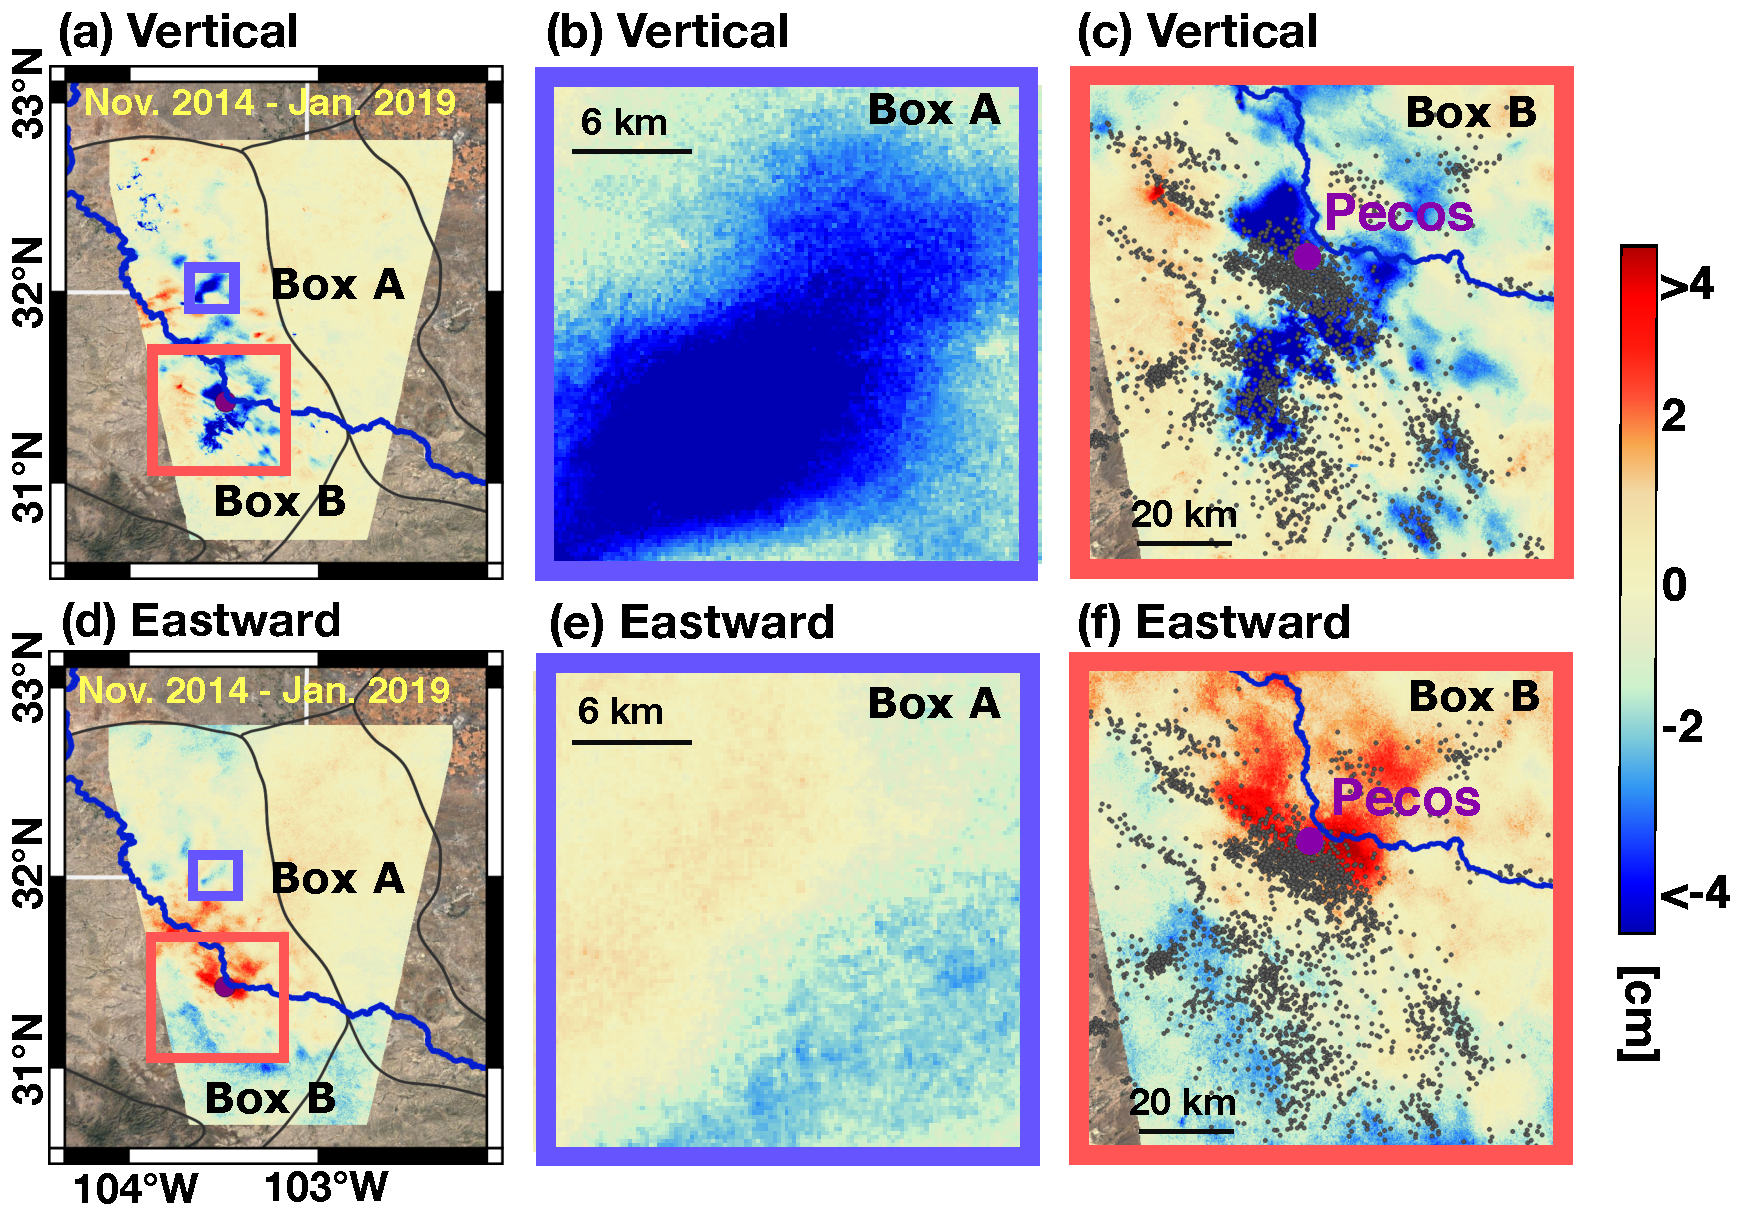
\includegraphics[width=0.96\linewidth]{paper1-permian/figures/figure4-east-vertical-6panel-labelled.pdf}
	\caption[Cumulative vertical and horizontal deformation]{(a) Cumulative vertical deformation between Nov. 2014 and Jan. 2019 over the region where Sentinel-1 path 78 and path 85 overlap. A zoomed-in view of Box A in the northern Delaware Basin and Box B in the southern Delaware Basin are shown in panel (b) and (c) respectively. (d) Cumulative eastward deformation between Nov. 2014 and Jan. 2019 over the region where Sentinel-1 path 78 and path 85 overlap. A zoomed-in view of Box A in the northern Delaware Basin and Box B in the southern Delaware Basin are shown in panel (e) and (f) respectively. In the southern Delaware Basin, the observed vertical and eastward deformation (panel (c) and (f)) show linear patterns along with earthquake hypocenters (gray dots) detected by TexNet in 2018.}
	\label{fig:insar-decomp}
\end{figure}


\subsection{Implications for geomechanical modeling}
Based on fault plane solutions derived from recent seismic activity and the faulting stress regime interpretations \cite{LundSnee2018}, the Pecos area is in a normal faulting regime. We employed an elastic dislocation model \cite{Okada1992} to demonstrate that the presence of dip-slip normal faults can produce the observed linear subsidence patterns in this area (Figure \ref{fig:model} (a)). We solved for the dip angle, depth, width along the dip direction, and slip magnitude of four normal faults by best fitting the forward model to InSAR vertical deformation observations, minimizing the sum of squared residuals, and maximizing the r-squared values \cite{Du1992} (\textit{Supporting Information S6}). The optimal solution suggests that the depth of the faults ranges from 0.9 km to 1.5 km, which is shallower than most of the TexNet recorded earthquakes (2-6 km in depth). Possible explanations for this discrepancy include: (1) the existence of aseismic fault slippage being responsible for the observed surface deformation \cite{mcgarr2018injection}; (2) bias in earthquake depth estimation in the TexNet catalog \cite{Lomax2019}; (3) systematic modeling errors associated with representing a mechanically layered earth as a homogeneous half space \cite{Du1992}. 



\begin{figure}[hbt!]
	\centering
	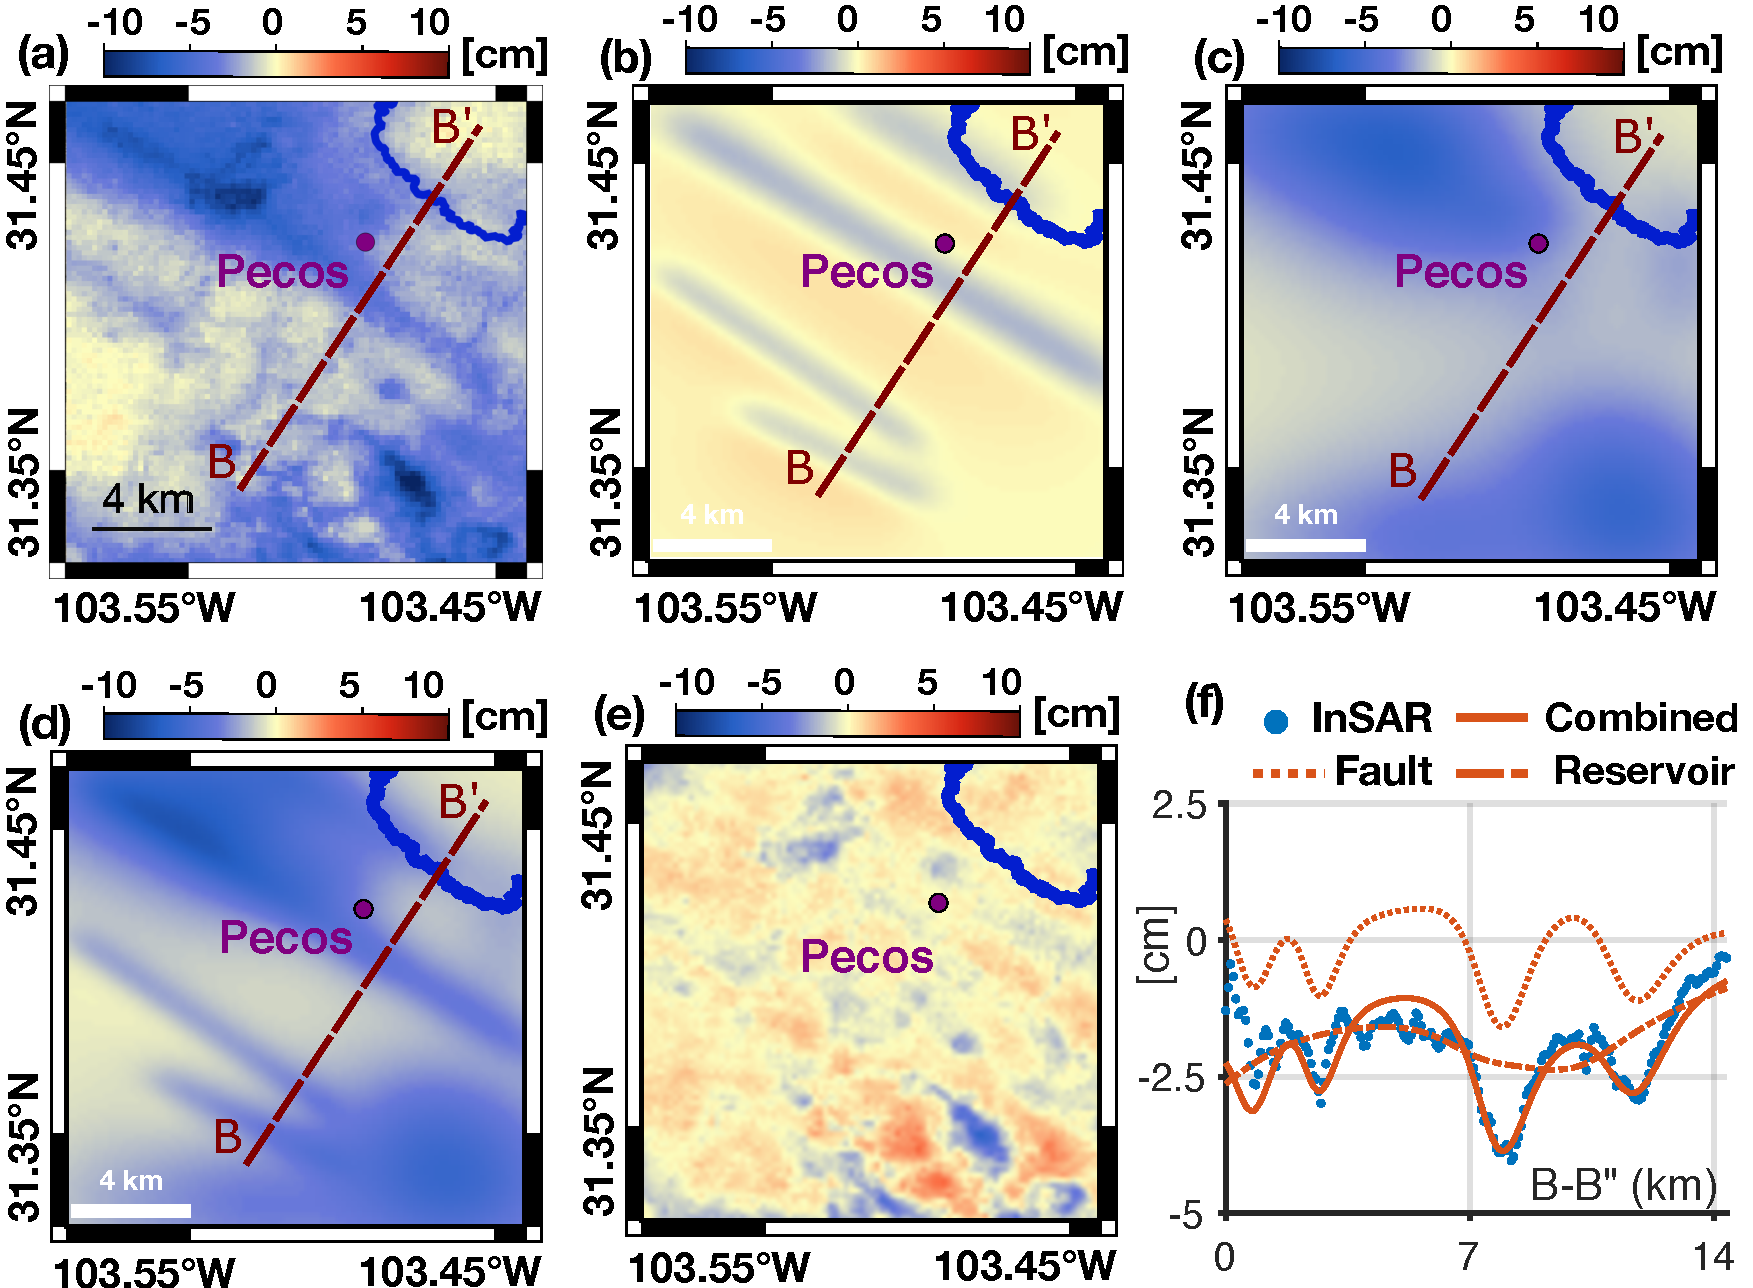
\includegraphics[width=\linewidth]{paper1-permian/figures/figure5-modeling.pdf}
	\caption[Modeled surface deformation from fault slip and reservoir subsidence]{(a) InSAR-observed cumulative vertical deformation between Nov. 2014 and Jan. 2019 in the Pecos, TX area. (b) Modeled vertical deformation associated with four dip-slip faults. (c) Modeled vertical deformation associated with reservoir compaction. (d) Modeled total vertical deformation associated with four dip-slip faults and reservoir compaction (panel (b) $+$ panel (c)). (e) Difference between InSAR-observed and model-predicted vertical deformation (panel (a) $-$ panel (d)). (f) Difference between InSAR-observed and model-predicted vertical deformation along the B-B' transect.}
	\label{fig:model}
\end{figure}


After removing the best-fit deformation associated with dip-slip faulting (Figure \ref{fig:model} (b)), there is still $\sim$ 2 cm residual subsidence in the Pecos area (e.g. Figure \ref{fig:model} (f)). Given that shallow groundwater production was minimal in this region for the time period of interest \cite{deng2020surface}, we introduced an elastic reservoir compaction model \cite{Geertsma1973} to our geomechanical analysis (\textit{Supporting Information S7}). We implemented two layers of multiple cylindrical reservoirs corresponding to reported locations and depths of well clusters in the Delaware Mountain Group (DMG) and Wolfcamp reservoirs, which account for most of the recent oil and gas production in the region. We discretized the DMG layer based on a cluster of production wells predominantly perforated over a depth range of 1.5-1.8 km. The Wolfcamp wells are completed over a depth range of 3-3.6 km. We employed an objective function inversion method to solve for the reservoir pressure depletion pattern that best fit the InSAR-observed subsidence (Figure \ref{fig:model} (c)) \cite{Du2001}.

An important conclusion of this study is that both fault slip and reservoir inflation or compaction can produce observable surface deformation over an 80,000 square kilometer oil-producing region of the Permian Basin. The InSAR-observed subsidence patterns over the Pecos area can be modeled as slip over multiple faults and discretized cylindrical reservoir compaction (Figure \ref{fig:model} (d)-(f)). We note that InSAR subsidence data alone can constrain all pertinent fault and reservoir parameters in our normal faulting and reservoir compaction models. The InSAR observed cumulative surface deformation patterns, which show larger horizontal component than the model prediction, suggest that other factors, such as strike-slip faulting and heterogeneity in subsurface properties, may play a role. There have been extensive studies on how reservoir compaction and inflation as well as fault slippage alter stress fields in the subsurface and produce surface deformation \cite{Geertsma1973, Segall1992, Okada1992, Du1992,Vasco2005, Vasco2008, Khakim2012}. InSAR surface deformation can be combined with this knowledge to evaluate fluid recovery efficiency and monitor disposal wells at low cost. Furthermore, these high-quality geodetic measurements are readily available to complement the TexNet seismic catalog for assessing the likelihood of fault motion and induced earthquake risks in Texas.






\chapter{Atmospheric Noise Analysis and Simulation}
\label{chap:atmo-noise}



Ideas:

- comparison of ways people have tried to correct for troposphere

- plots/images of possible views into the single day atmosphere.
 -- modis
 -- HRRR, ECMWF
 --  GOES
 -- insar averaging
 
 axes of comparison:
 - resolution
 - time availability
 - spatial availibility
 - sensitivity to phase propation delay
 
 
 SEASONAL plots...
 
 Note


\chapter{Automatic Detection of InSAR Surface Deformation Signals In the Presence Severe Tropospheric Noise}


\section{Methods}
\label{sec:methods}

% \subsection{Overview}
% \label{subsec:methods-overview}


\subsection{Automatic Feature Detection}
\label{subsec:methods-1-log}

Given a surface deformation map $M$ derived from InSAR data, the value $ M_{ij} $ at the $i^{th}$ row and $j^{th}$ column represents the magnitude of a cumulative, seasonal, or transient deformation signal at this pixel. Because the earth can be considered as a stratified elastic-viscoelastic medium, surface deformation features in an InSAR map are often spatially coherent \citep{Segall2010EarthquakeVolcanoDeformation}.

There have been many computer vision algorithms that were designed to automatically detect spatially coherent ``blob-like'' features in 2D image data \citep{Lindeberg1993DetectingSalientBlob, Lindeberg1998FeatureDetectionAutomatic, Lowe2004DistinctiveImageFeatures}. Here we employ the Laplacian of Gaussian (LoG) filters as a blob detector. An LoG kernel $K^{(m)}$ with a size $\sigma_m$ is written as:
\begin{equation}
K^{(m)}_{ij} = \left(\frac{(i - l)^2 + (j - l)^2 - 2\sigma_m^2}{2 \pi \sigma_m^4}\right) \, e^{-\frac{ (i - l)^2 + (j - l)^2}{2 \sigma_m^2}} \label{eq:log-kernel}
\end{equation}
where pixel indices $ij  \in \left\lbrace 0, 1, \ldots, 2l \right\rbrace$. The unit of $\sigma_m$ is given in pixels, which can be scaled to meters based on the pixel spacing of the InSAR deformation map $M$.
% and $l$ is a kernel size chosen to be sufficiently larger than $\sigma_n$ such that the edge pixels approach 0. 
%is a matrix of size $ (2l + 1, 2l + 1) $ whose value in the $i$th row and $j$th column is given by
%The kernel is derived by taking spatial second derivatives of a Gaussian smoothing kernel, then normalizing with an extra factor of $\sigma_n^2$ so that kernels with both small and large $\sigma_n$ produce comparable filter responses. 

%Each kernel is sensitive to deformation features which roughly match the radius of the kernel. The radius $ r_n $ of a circularly symmetric feature with the highest sensitivity to kernel $K^{(n)}$ can be calculated as $ r_n = \sqrt{2}\sigma_n $.

We generate a set of LoG kernels $K^{(1)}, K^{(2)}, \ldots$ with progressively larger $\sigma_m$ (Figure \ref{fig:log-kernel}), and calculate the $m^{th}$ filter response $ L^{(m)} $ as:
\begin{equation}
L^{(m)} = M \ast K^{(m)}  \label{eq:log-layer-conv}
\end{equation}
%However, this operation is computationally expensive for larger kernels; thus, the filtering is carried out in the Fourier domain.
Here $*$ denotes the 2D discrete convolution, which is typically computed using the Fast Fourier Transform (FFT) algorithm because of its superior computational efficiency \citep{Szeliski2022ComputerVision}.

To demonstrate how to estimate the size of an unknown deformation feature, Figure \ref{fig:log-response} (a) shows a $500 \times 500$ synthetic deformation map $M$ that contains one Gaussian-shaped uplift feature in the upper left and one elliptical Gaussian subsidence feature in the lower right. We filtered this deformation map using 20 LoG kernels of sizes ranging from $\sigma_1 = 3$ pixels to $\sigma_{20} = 100$ pixels with a base-2 logarithmic spacing, and the filter responses are shown in Figure \ref{fig:log-response} (b)-(e). For the round uplift case, the filter response $L^{(m)}$ (the black curve in Figure \ref{fig:log-response} (b)) is strongest when the kernel size $\sigma_m$ matches the deformation feature radius $r$ as $r = \sqrt{2}\sigma_m$. This is known as the extreme point, or the local maximum points of $|L^{(m)}|$ for all attempted $\sigma_m$. For the elliptical subsidence case, the extreme point is reached when the average length of the two primary axes of the deformation feature is $\sim \sqrt{2}\sigma_m$ (the green curve in Figure \ref{fig:log-response} (b)). For the case of no deformation, no substantial filter response is generated for any filter size (the gold curve in Figure \ref{fig:log-response} (b)).
	
\begin{figure}[hbt!]
\centering
 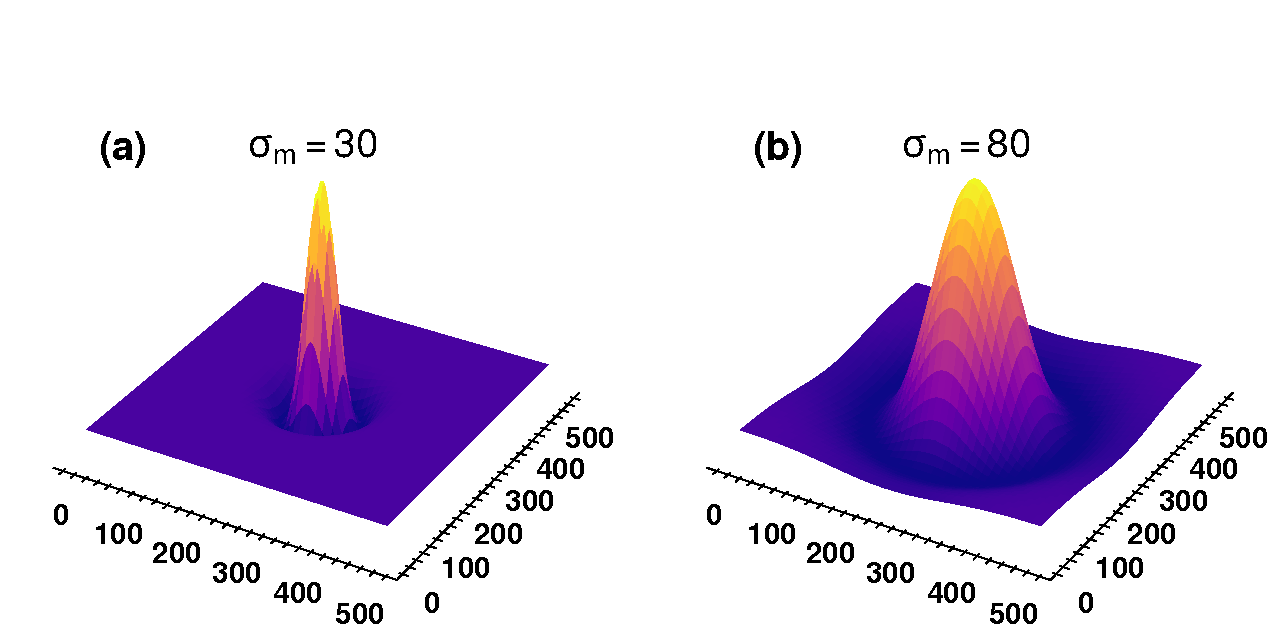
\includegraphics[width=0.98\linewidth]{paper2/figures/figure1_log_examples.pdf}
\caption[Laplacian of Gaussian (LoG) kernels]{
Laplacian of Gaussian (LoG) kernels with (a) $\sigma_m=30$ pixels and (b) $\sigma_m=80$ pixels for an image of size of 500-by-500 pixels.
}
\label{fig:log-kernel}
%
\end{figure}

\begin{figure}[hbt!]
\centering
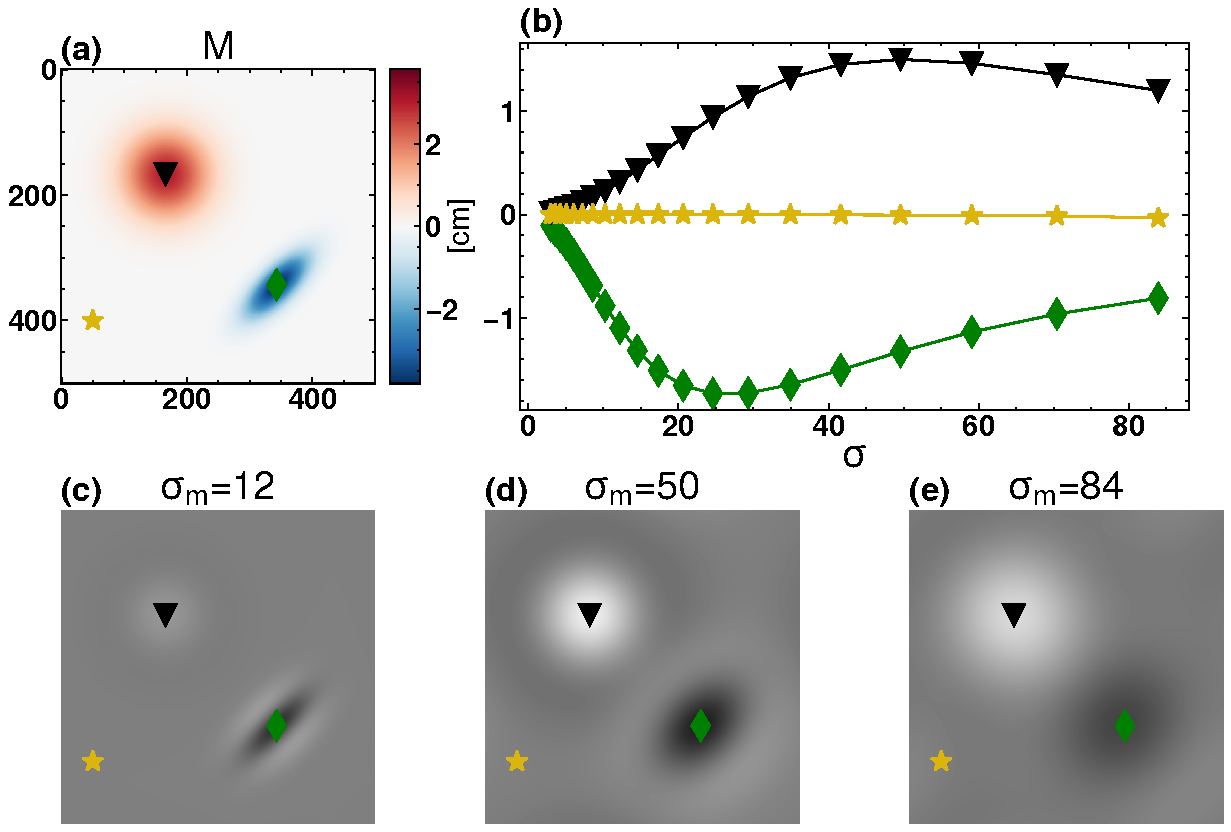
\includegraphics[width=0.98\linewidth]{paper2/figures/figure2_log_response.pdf}
\caption[LoG filter responses]{
(a) A synthetic deformation map that contains one Gaussian-shaped uplift feature in the upper left and one elliptical Gaussian subsidence feature in the lower right. (b) LoG response amplitudes for 20 filters with various sizes ($\sigma_m$) at three marker points. The marker locations are shown in panel (a). (c)-(e) The LoG filter responses for $\sigma_m=$ 12, 50, and 84.}
\label{fig:log-response}
%
\end{figure}

%Paragraph 3 : Ghost blob removal
%To obtain the final detection results, we add two additional steps to remove undesirable detection candidates. 
% (Figure \ref{fig:log-response}e, bottom right).% (Figure \ref{fig:log-response}e, upper right).
In the case that two candidate blobs have more than 50\% overlapping area, the blob with a smaller size is discarded. 
Additionally, the LoG filter may falsely flag ghost blobs at the edges of real deformation features. This is because deformation features with strong curvature at the center also contain a strong opposite-signed curvature near the border \citep{Lindeberg1998FeatureDetectionAutomatic}. To remove those false positives, we use the distance from the candidate blob's center location to the nearest deformation amplitude extremum as a measure. If this distance is close to the blob radius, the detection is likely a ghost blob. In our test case, we discarded blobs with local extremum distances larger than 75$\%$ of the blob radius, which effectively removed all visible false positives near the edge of real deformation features.

For the $k$th detected deformation feature, our algorithm outputs the blob center location $(i_k, j_k)$, the blob radius $ r_k$, the filter response magnitude $|g_k|$ at the extreme point, and the deformation magnitude $|\bar{d_k}|$ defined as the weighed maximum of all pixels within the $k^{th}$ blob:
\begin{equation}
\bar{d_k} = \max_{kk} |w_{kk} M_{kk} | 
\end{equation}
Here the weight $w_{kk}$ equals $\exp\left[-(r_{kk} / r_k)^2\right]$, where $r_{kk}$ is the distance between a pixel within the blob and the blob center. The exponential weighting prevents pixel outliers from distorting the measure of feature magnitude. 

We can exclude undesired deformation features by setting magnitude thresholds on $|g_k|$ and $|\bar{d_k}|$ based on users' interest. Furthermore, we need to determine whether a detected deformation feature has a signal magnitude above the noise level of the InSAR deformation map, which is the focus of the following method sections. 


\begin{algorithm} [htb]
\caption{LoG Based Deformation Feature Detection}\label{algo:blobs}
\SetAlgoLined
\KwIn{2D InSAR deformation map $M$}
\KwResult{For each $k \in {1, \ldots, N_d}$ detections, the algorithm outputs the blob center location $ (i_k,j_k) $, the blob radius $ r_k $, the filter response magnitude $|g_k|$ at the extreme point, the deformation magnitude $|\bar{d_k}|$ }


// Calculate filter responses:\\
\ForEach{$ \sigma_m \in \left\lbrace \sigma_{min} \ldots \sigma_{max}\right\rbrace $}{
%$L^{(n)} = \mathcal{F}^{-1} \left[ \mathcal{F} M \cdot  \mathcal{F} K^{(n)} \right] $
$ L^{(m)} = M \ast K^{(m)}  $
%$\nabla^2_{norm} L(\cdot, \cdot, \sigma) \gets I(\cdot, \cdot) * \nabla^2_{norm} G(\cdot,\cdot, \sigma)$
}

// Find candidate blobs from local extrema:\\
\For{$ (i, j, m) \in  L $}{
	\If{$L[i, j, m] $ is local extremum }{
    % \If{$\det \mathcal{H}_{norm} L(x,y,\sigma ) $ is local extremum }{
		Compute $ r = \sqrt{2}\sigma_m $ \\
		Add $ (i, j, r) $ to list of candidate detections
	}
}
// Prune blobs with overlap:\\
\ForEach{$ b_1 := (i_1, j_1, r_1), b2 := (i_2, j_2, r_2) \in $ candidates}{
%	Form circle of radius $ r_i $ around $ (i_1, j_1) $\\
	\If{ Overlap$( b_1, b_2 ) > 0.5 $  }{
		Remove smaller of $ b_1, b_2 $
	}
}

// Prune edge blob false positives:\\
\ForEach{$ b_k := (i_k, j_k, \sigma_k) \in $ candidates}{
    Find coordinates $(u, v)$ of local max of $M$ within
    radius $r_k$ around $ (i_k, j_k) $
    \\
    \If{ $\sqrt{(x - u)^2 + (y - v)^2} > 0.75 $  }{
		Discard $ b_k $
	}
}
// Prune with thresholds $ \gamma_g, \gamma_d $:\\
\ForEach{$ b_k := (i_k, j_k, r_k,|g_k|, |\bar{d_k}|) \in $ candidates}{
	\If{ $ |g_k| <  \gamma_g $ \text{or} $ |\bar{d_k}| <  \gamma_d $  }{
		Discard $ b_k $
	}
}
\end{algorithm}



\subsection{Tropospheric Noise Spectrum}
\label{subsec:methods-2-tropo-spectrum}
 InSAR measurement noise can also produce spatially coherent "blob-like" features that are detectable by our algorithm.  Here we focus on characterizing the tropospheric turbulence noise in each SAR scene. This is because tropospheric turbulent noise (1) is correlated in space; (2) is present in all InSAR data sets with greatly varying magnitudes; and (3) is often the primary noise source that limits InSAR measurement accuracy \citep{Bekaert2015StatisticalComparisonInsar}.

% tropospheric turbulence noise occurs in all study regions globally, and is often the dominant error source even in cases where decorrelation is non-negligible.
%Even if a study area has regions containing decorrelation, the resulting noise does not appear as a blob-like feature and is unlikely to our algorithm. 

Consider an interferogram formed using two SAR scenes acquired at times $t_1$ and $t_2$. In the case that tropospheric turbulence noise is the dominant noise term, the measured interferometric phase $\phi_{1,2}$ (in radians) at a pixel of interest can be written as \citep{Zebker1997AtmosphericEffectsInterferometric}:
\begin{equation}
\phi_{1,2} \approx \frac{4 \pi}{\lambda} \left(\alpha_2 - \alpha_1 + \Delta d_{1,2} \right)
\end{equation}
where $ \lambda $ is the radar wavelength, $\alpha_1$ and $\alpha_2$ represent the tropospheric delay at the two SAR acquisition times $t_1$ and $t_2$, and $\Delta d_{1,2} $ is the Line-Of-Sight (LOS) deformation ($d_2-d_1$) between $t_1$ and $t_2$. The unit of $\lambda$, $\alpha_1$, $\alpha_2$, and $\Delta d_{1,2} $ is in centimeters. 

Given N SAR acquisitions, we can estimate the tropospheric noise on the $n^{th}$ SAR acquisition date by averaging $N-1$ interferograms that share the common reference SAR scene $n$ \citep{Tymofyeyeva2015MitigationAtmosphericPhase}:
\begin{multline}
\bar{\alpha}_n = \frac{\lambda}{4 \pi} \frac{1}{N-1} \left(\sum_{k=1, k \neq n}^{N} \phi_{k,n}\right)  \\
=  \alpha_n  + \frac{1}{N-1} \left( \sum_{k=1, k \neq n}^{N}  \Delta d_{k,n} - \sum_{k=1, k \neq n}^{N}  \alpha_k  \right)  \label{eq:avg-ifg} 
\end{multline}
%Note that the interferograms are all formed with $k$ as the reference date; any interferogram which was processed using $k$ as the secondary is multiplied by $-1$ before averaging. 
Because tropospheric turbulence noise is uncorrelated in time for scales longer than one day \citep{Emardson2003NeutralAtmosphericDelay, Onn2006ModelingWaterVapor}, the term $ \frac{1}{N-1} \sum \alpha_k \rightarrow 0$ when  when $N$ is sufficiently large. 
%Additionally, for uncertainty quantification, we are interested determining the size of the smallest possible detectable signal. This will typically be much smaller than the tropospheric turbulence noise on any given day, since InSAR time series analysis can reduce tropospheric turbulence noise by a factor of $\sqrt{N}$ \citep{Sandwell1998PhaseGradientApproach}. Thus, the residual deformation term $  \frac{1}{N-1}  \sum  \Delta d_{k, m} $ does not significantly affect our estimation of the noise $\alpha_n$. 
%Additionally, in the cases where we're interested in automatically detecting unknown deformation signals, the deformation $\Delta d_{n,k}$ is small (sub-centimeter). In any given interferogram, the noise $\alpha_n$ has much more power than the local deformation features, and thus is not a substantial component in the characterization.
Under the assumption that $ \frac{1}{N-1} \sum \Delta d_{k,n} $ is relatively small comparing to $\alpha_n$, we compute $ \bar{\alpha}_n $ at each pixel to obtain a tropospheric turbulence noise map $A^{(n)}$ for the $n^{th}$ SAR acquisition date over the entire study area. In Section \ref{subsec:discussion-residual-deformation}, we further discuss the impact of the deformation signals on our tropospheric noise analysis.
%We then use spectral analysis on $A^{(n)}$ to further estimate the noise \citep{Hanssen2001RadarInterferometryData}. Figure \ref{fig:psd-example}a shows an example of one day's tropospheric turbulence noise estimate for a $ 500 \times 500 $ pixel map with $100$ meter pixel spacing. The noise is spatially correlated with a peak-to-peak amplitude of several centimeters. 

We next compute the 2D Power Spectral Density (PSD) of the $n^{th}$ tropospheric noise estimates at  wavenumber $ k_x, k_y $ (with units $1/m$) as \citep{Jacobs2017QuantitativeCharacterizationSurface}:
\begin{equation}
\text{PSD}_n(k_x, k_y) = \frac{| \widehat{A^{(n)}} |^2 }{N_x N_y (\frac{1}{\Delta x \Delta y}) } \label{eq:pow-spec}
\end{equation}
where  $\widehat{A^{(n)}}$ is the Discrete Fourier transform (DFT) of  the $n^{th}$ tropospheric noise map $A^{(n)}$, $\Delta x$ and $\Delta y$ are the interferogram pixel spacings (in meters) in the $x$ and $y$ directions, $N_x$ and $N_y$ are the total number of pixels in the $x$ and $y$ directions, and the squared absolute value and division are pixel-wise operations. 


%The arguments $k_x, k_y$ are 2D spatial frequency coordinates (also called the wavenumber) with units $1/m$. 
%The result is shown in Figure \ref{fig:psd-example}b. The majority of the noise power is at low spatial frequencies (near the origin), and at higher frequencies, the PSD drops off as a power law \citep{Hanssen2001RadarInterferometryData}. 

Here we use an example to demonstrate how to estimate the PSD of a 2D tropospheric turbulence noise map (Figure \ref{fig:psd-example} (a)). First, we calculate the 2D PSD of the noise map following Equation \eqref{eq:pow-spec} (Figure \ref{fig:psd-example} (b)). Under the assumption that tropospheric noise is isotropic, we average all pixels with a distance  $k= \sqrt{k_x^2 + k_y^2}$ from the origin to generate a 1D PSD as a function of $k$ \citep{Hanssen2001RadarInterferometryData}.
%The vertical dashed line in Figure \ref{fig:psd-example}c marks a reference frequency $k_0$ where the power level $P_0$ is measured to compare the power of tropospheric turbulence noise on different days. 
%We parameterize $ \text{PSD}_n(k) $ by fitting a cubic polynomial to $ \log ( \text{PSD}_n(k) )$ vs. $\log (k) $ \citep{Treuhaft1987effectdynamicwet}. 
%The cubic polynomial accounts for the varying power-law slopes of the three turbulence regimes in \citep{Hanssen2001RadarInterferometryData}, which are derived from Kolmogorov turbulence theory. Finally, 
Here the 1D PSD is plotted on a log-log scale, which rolls off following a power law at higher frequencies (Figure \ref{fig:psd-example} (c)). By contrast, the power spectrum of spatially uncorrelated while noise is relatively flat across all frequencies $k$ (Figure \ref{fig:psd-example} (d)-(f)).

%To produce a single atmospheric noise curve $\tilde{P}(k)$ for the study region, we average all dates' power spectra and fit a polynomial to this averaged spectrum. This curve has a shape and power level which reflects the characteristics of the study area's atmospheric noise. 


\begin{figure}[hbt!]
\centering 
%\includegraphics[width=0.98\linewidth]{figures/figure3_psd_radial.pdf}
\includegraphics[width=0.98\linewidth]{paper2/figures/figure3_psd_radial.png}
\caption{
(a) A simulated 2D turbulent atmospheric noise map with $ 500 \times 500 $ pixels at $100$ meter pixel spacing.
(b) 2D Power Spectral Density (PSD) of the tropospheric noise map in panel (a) computed using Equation \eqref{eq:pow-spec}.
(c) 1D PSD as a function of wavenumber $k = \sqrt{k_x^2 + k_y^2}$ derived from panel (b), under the assumption that tropospheric noise is isotropic.
(d) A simulated 2D white noise map (spatially uncorrelated) with the same dimension and pixel spacing as panel (a)
(e) 2D PSD of the white noise map in panel (d) computed using Equation \eqref{eq:pow-spec}.
(f) 1D PSD as as a function of wavenumber $k = \sqrt{k_x^2 + k_y^2}$. Here We averaged the 1D PSD of 50  2D white noise instances to improve the statistical stability of the spectral estimates.
}
\label{fig:psd-example}
\end{figure}



\subsection{Uncertainty Quantification}
\label{subsec:methods-3-noise-sim}

Using the average 1D PSD of all $N$ InSAR-observed tropospheric turbulence noise maps, we can simulate $N$ noise incidences  $S^{(1)},\dots, S^{(N)} $ that closely resemble the real tropospheric noise over the study area \citep{Hanssen2001RadarInterferometryData}. Using these simulated noise maps, we form up to $N(N-1)/2$ noise-only interferograms, and derive a time series solution following the same method that is used for generating the real InSAR deformation map $M$ (e.g. \citep{Sandwell1998PhaseGradientApproach, Berardino2002NewAlgorithmSurface}). Because these synthetic interferograms contain no deformation, any "blob-like" features in the simulated time series solution are associated with tropospheric noise. We record the radius $r_k$,  filter response magnitude $|g_k|$ and deformation magnitude $|\bar{d_k}|$ of each noise feature using our automatic blob detection algorithm.

Similarly, we generate many synthetic InSAR data sets that share the same noise spectrum derived from data, and record all detected noise blobs. We create 2D histograms of the noise attributes (filter response magnitude vs. radius and deformation magnitude vs. radius), which allows us to remove candidate blob features in the real deformation map $M$ that are likely due to tropospheric noise artifacts.

\section{Test Site and Available InSAR Data}
\label{sec:site}

We tested our deformation detection algorithm on over an 80,000 $km^2$ oil-producing region in the Permian Basin, West Texas.  As described in \citep{Staniewicz2020InsarRevealsComplex}, we processed 84 ascending (path 78, frames 94–104) Sentinel-1 scenes acquired between November 2014 and January 2019 (Figure \ref{fig:study-area}). We imposed no maximum spatial baseline and a maximum temporal baseline of 800 days for interferogram selection, resulting in 2550 multi-looked interferograms with 120 m pixel spacing.  We used the GPS station TXKM as the reference location, where little surface deformation was observed over the study period (Figure \ref{fig:study-area}, yellow dot).

We employed a stacking approach \citep{Sandwell1998PhaseGradientApproach, Staniewicz2020InsarRevealsComplex} to calculate the average LOS velocity $v_{avg}$ of each ground pixel over a time period of interest $ T $ as
\begin{equation}
v_{avg} = \frac{\sum_{i \in G} d_i}{\sum_{i \in G} t_i}
\label{eq:stacking}
\end{equation}
where $G$ is a subset of interferograms formed using two SAR scenes acquired within the time period $T$. The LOS measurement (in cm) and the temporal baseline of the $i^{th}$ interferogram in $G$ are written as $d_i$ and $ t_i $ respectively.
For example, we used 29 SAR scenes acquired between November 2014 and January 2017 to solve for the average velocity during this period, and we computed the cumulative deformation as the average velocity times the total time span ($\sim 2 years$). Similarly, we used 52 SAR scenes acquired between November 2014 and January 2018, and 84 SAR scenes acquired between November 2014 to January 2019 to derive the cumulative deformation maps over these two study periods.


\begin{figure}[hbt!]
\centering
%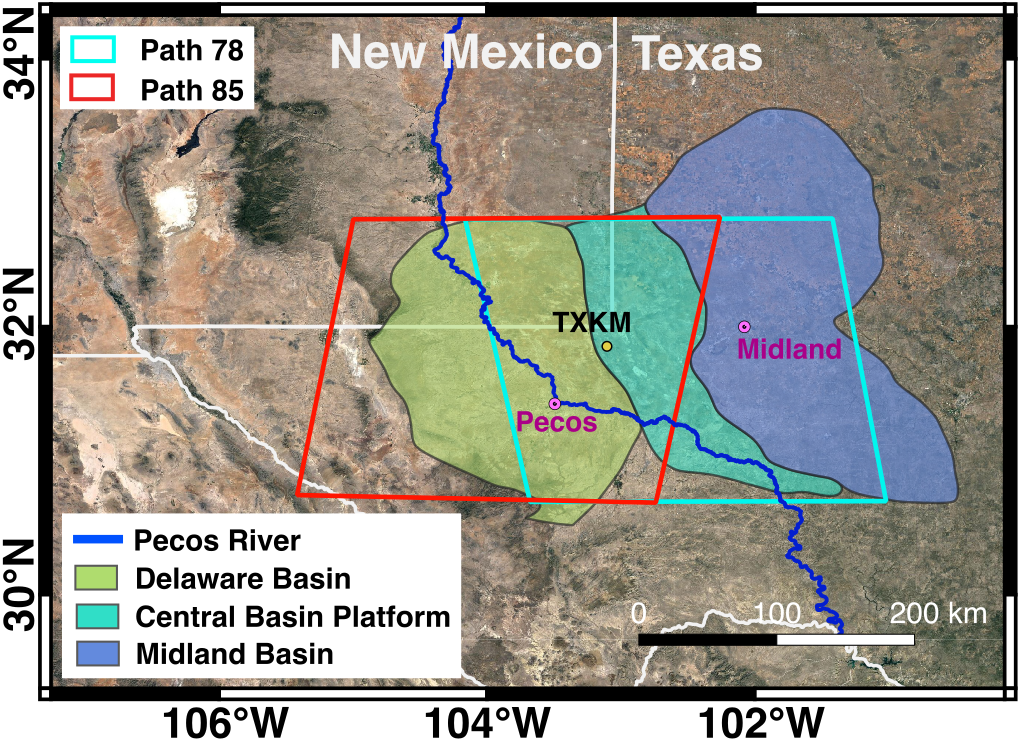
\includegraphics[width=0.9\linewidth]{paper2/figures/figure4-study-area.pdf}
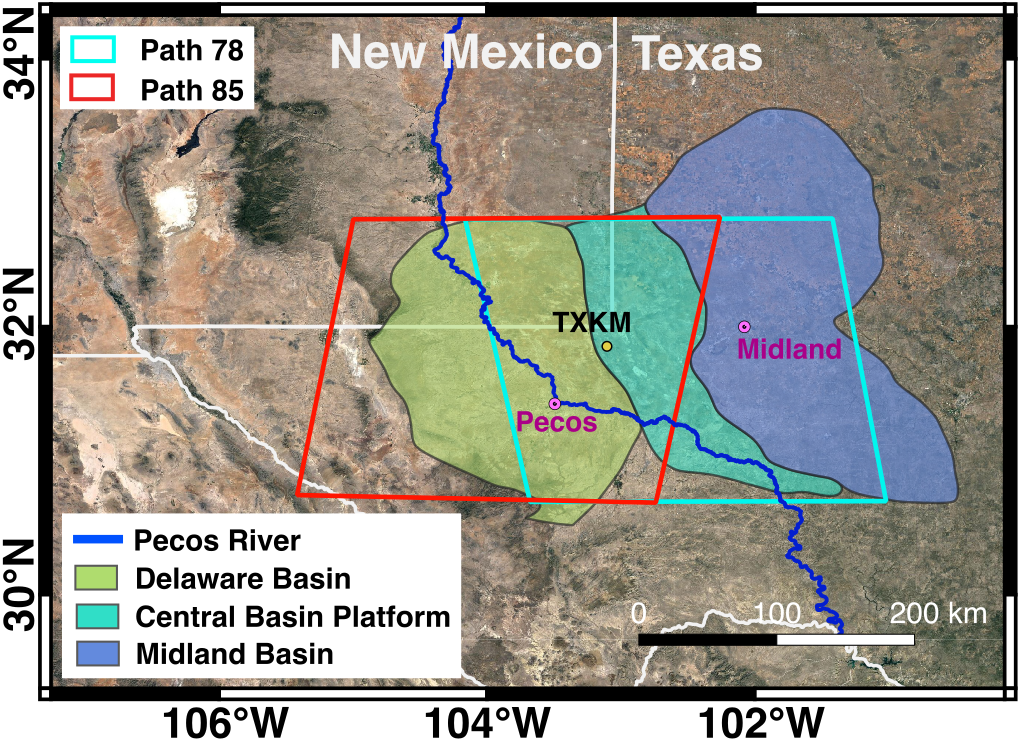
\includegraphics[width=0.96\linewidth]{paper2/figures/figure4-study-area.png}
\caption{GPS and InSAR data coverage over the Permian Basin. Teal and red boxes indicate ascending path 78 and descending path 85 paths of Sentinel 1 InSAR coverage, respectively. GPS station TXKM (yellow dot) was used as the reference point for both paths.
%Each path contains over 80 SAR acquisitions, leading to over 3500 interferograms per path at 180 m pixel spacing.
}
\label{fig:study-area}
\end{figure}

We estimated the tropospheric turbulence noise for the $n^{th}$ SAR acquisition date using all interferograms that contain this SAR scene. (Equation \eqref{eq:avg-ifg}). We removed a quadratic ramp in each noise map, and calculated the average 1D PSD of all 84 noise maps as described in \ref{subsec:methods-2-tropo-spectrum}.
%The 800 day temporal baseline resulted in up to $\sim$80 interferograms per acquisition near the middle of the time period (which have 800 days available before and after the date).
Using the average noise spectrum, we generated 29 synthetic noise maps, which corresponds to the 29 Sentinel-1 acquisition dates between November 2014 and January 2017. We formed noise-only synthetic interferograms and calculated the cumulative stacking solution using Equation \eqref{eq:stacking}. We ran our blob detection algorithm on the noise-only stacking solution, and recorded the size, filter response magnitude, and deformation magnitude of each detected blob feature. We counted the total number of detections, and created 2D histograms of the noise attributes (filter magnitude vs. radius, and deformation magnitude vs. radius) for the Sentinel-1 November 2014-January 2017 solution.
%We call this entire procedure one simulation, and we call the resulting set of detections one synthetic dataset. 
Similarly, we ran additional simulations to create 2D histograms of the noise attributes (filter magnitude vs. radius, and deformation magnitude vs. radius) for the November 2014-January 2018, and November 2014-January 2019 solutions.
%We repeated this simulation for the Nov. 2014 - Jan. 2018 time period using 52 simulated tropospheric turbulence maps, and for the Nov. 2014 - Jan. 2019 time period using 84 simulated tropospheric turbulence maps.
%we performed 3 rounds of simulation: one for the 2-year, 3-year, and 4-year cumulative deformation maps. For each round, we generated the same number of synthetic tropospheric turbulence noise maps as Sentinel-1 acquisitions.  
These histograms were then used to remove candidate blob features in the real Sentinel-1 InSAR deformation maps that are likely due to tropospheric noise artifacts.

We also processed 81 descending Sentinel-1 scenes for path 85 (frames 483–493) (Figure \ref{fig:study-area}, red box) acquired between November 2014 and January 2019 as described in \citep{Staniewicz2020InsarRevealsComplex} using the the same GPS station TXKM as the reference location. Following the same processing strategy, we estimated three cumulative deformation maps spanning November 2014 to January 2017, January 2018, and January 2019. We characterized the tropospheric noise from InSAR data, and identified deformation features in the cumulative deformation maps that are likely real.

\section{Results}
\label{sec:results}
%\subsection{Tropospheric Noise Power Spectra}

The strength of the tropospheric turbulence noise estimated for path 78 varies by over an order of magnitude (Figure \ref{fig:results-noise}). Example noise maps are shown for the SAR acquisitions on dates 2017-12-12 (Figure \ref{fig:results-noise}a), 2018-09-14 (Figure \ref{fig:results-noise}c), and 2017-06-15 (Figure \ref{fig:results-noise}c), which illustrate days of weak, medium, and strong tropospheric noise. Each map contains turbulence features ranging from a few kilometers up to tens of kilometers in diameter.  
We measured the peak amplitude of all 84 noise maps, where the peak is defined as the maximum of the absolute values of all pixels (Figure \ref{fig:results-noise}d). 
For example, the peak amplitudes from (Figure \ref{fig:results-noise}(a), (b) and (c) are 1.8 cm, 3.2 cm, and 12.6 cm, respectively.  Approximately 50\% of SAR acquisitions have quiet atmospheric conditions with a peak noise level under 4 cm, 35\% have moderate turbulence, with a peak between 4-10 cm, and $\sim$15\% of the SAR acquisitions have strong tropospheric noise peaks of 11-15 cm. 

Since InSAR measure deformation relative to a reference point, for each noise map, we re-referenced the noise maps to the center pixel and took the mean absolute value of the noise vs. distance to the reference (Figure \ref{fig:results-noise}(e)). The majority of acquisitions show a roughly square root growth of noise vs. distance to the reference, with a flattening of noise at ranges $>60-70$ km. The strongest noise days show a sharper rise of noise strength at short distances from the reference, and show longer length scales before flattening.


The 1D PSDs for the 84 tropospheric turbulence noise maps give an alternative view of the distribution of noise power (Figure \ref{fig:results-noise}(f). For most spatial frequencies, the PSDs decay following the -8/3 power law described in previous studies \citep{Hanssen2001RadarInterferometryData, Onn2006ModelingWaterVapor}. This slope flattens at the lowest frequencies, due to the quadratic phase removal, as well as at the highest frequencies, where pixel-level variations begin to dominate tropospheric fluctuations.



\begin{figure*}[hbt!]
\centering 
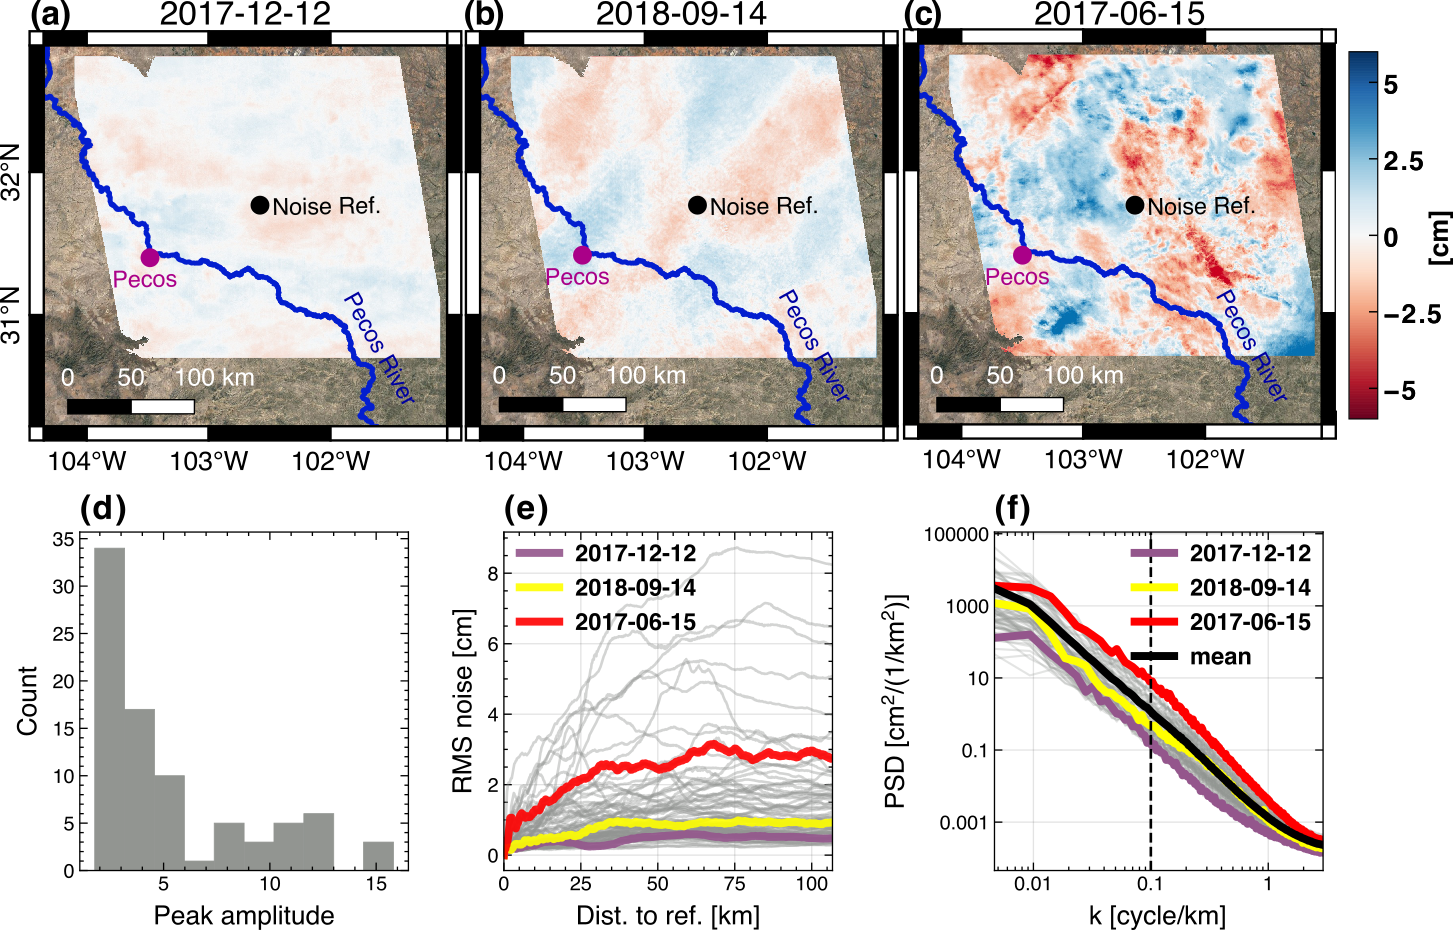
\includegraphics[width=0.98\linewidth]{paper2/figures/figure5_noise_path78.png}
%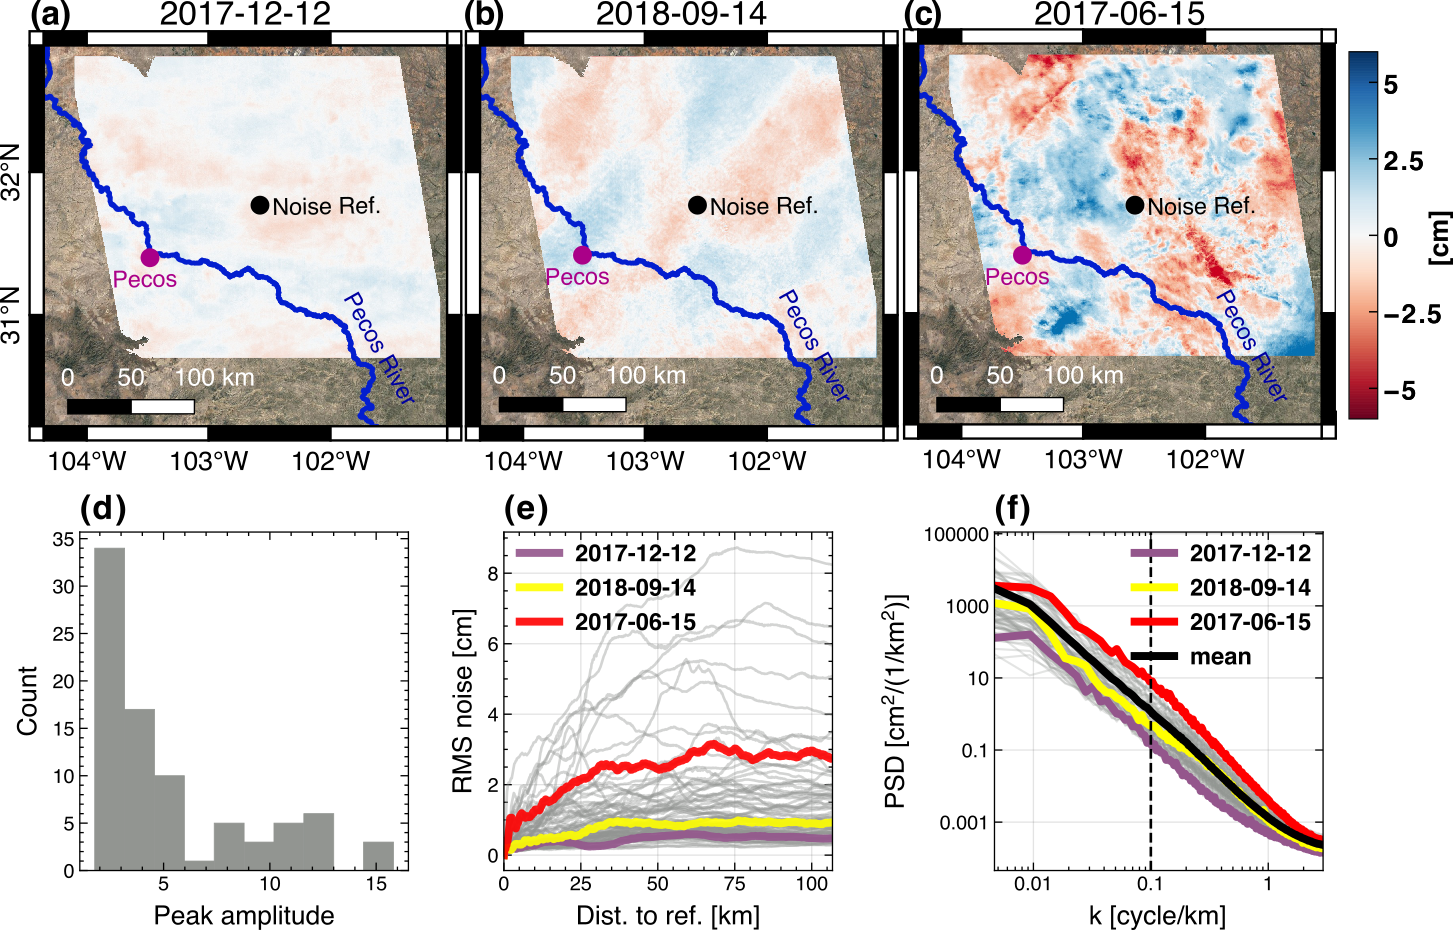
\includegraphics[width=0.98\linewidth]{paper2/figures/figure5_noise_path78.pdf}
\caption{Estimated tropospheric turbulence noise examples for path 78 SAR acquisitions on (a) 2017-12-12, (b) 2018-09-14, and (c) 2017-06-15.
(d) Histogram of peak absolute value for 84 estimated noise maps from path 78. The values from panels (a), (b) and (c) are 1.8 cm, 3.2 cm, and 12.6 cm, respectively. 
(e). Root mean squared value of noise vs distance from reference point for each noise map. Color lines represent the calculated noise curves for panels (a), (b), and (c).
(f) 1D PSDs for 84 SAR acquisitions from path 78 (gray lines), bold color lines correspond to example dates, and bold black line corresponds to the mean PSD. 
}
\label{fig:results-noise}
\end{figure*}


%\subsection{Simulated tropospheric turbulence noise and Uncertainty Quantification}

Using the mean 1D PSD shown in Figure \ref{fig:results-noise}(f), we simulated instances of tropospheric turbulence.
%(Figure \ref{fig:results-kde}(a-c)). The noise instances are spatially isotropic and contain many $\sim$3 cm blob-like features ranging from several km up to $\sim$100 km in length. 
As outlined in Section \ref{sec:site}, we computed LOS deformation maps from 29 noise instances, and we recorded all detected noise features. The resulting histograms of ($g$ vs. $r$ and $\bar{d}$ vs. $r$) were smoothed using a kernel density estimate (KDE) \citep{Scott2015MultivariateDensityEstimation} to create 2D empirical probability density functions (PDFs) (Figure \ref{fig:results-kde}). The PDFs shows a high concentration of detected features with small radii ($r <$ 5 km) with many more low amplitude features found than high amplitude features. For the 29 SAR acquisition case, the features are unlikely to be larger 2 cm in deformation amplitude (Figure \ref{fig:results-kde}(d)) or have a filter response stronger than 0.7 (Figure \ref{fig:results-kde}(a)). As the number of SAR acquisitions increases to 52 (Figure \ref{fig:results-kde}(b,e)) and 84 (Figure \ref{fig:results-kde}(c,f)), the amplitudes of detected features decreases for all $r$.

Note that the maximum and minimum $r$ of detected features in Figure \ref{fig:results-kde}(d-f) are limited by the choice of $\sigma_{max}, \sigma_{max}$ from our detection algorithm. By imposing the prior knowledge that oil and gas-production related deformation bowls are unlikely to be larger than 30-40 km across, $\sigma_{max}$ was set so that maximum radius $r$ was approximately 20 km. Thus, even though larger structures appear in the noise, these were not detected and recorded. Additionally, due to the averaging involved in computing the cumulative LOS deformation, the amplitudes of detected features shown in Figure \ref{fig:results-kde} are smaller than those appearing in the individual noise simulations.


\begin{figure*}[hbt!]
\centering 
%\includegraphics[width=0.98\linewidth]{paper2/figures/figure_results_simulation_kde.png}
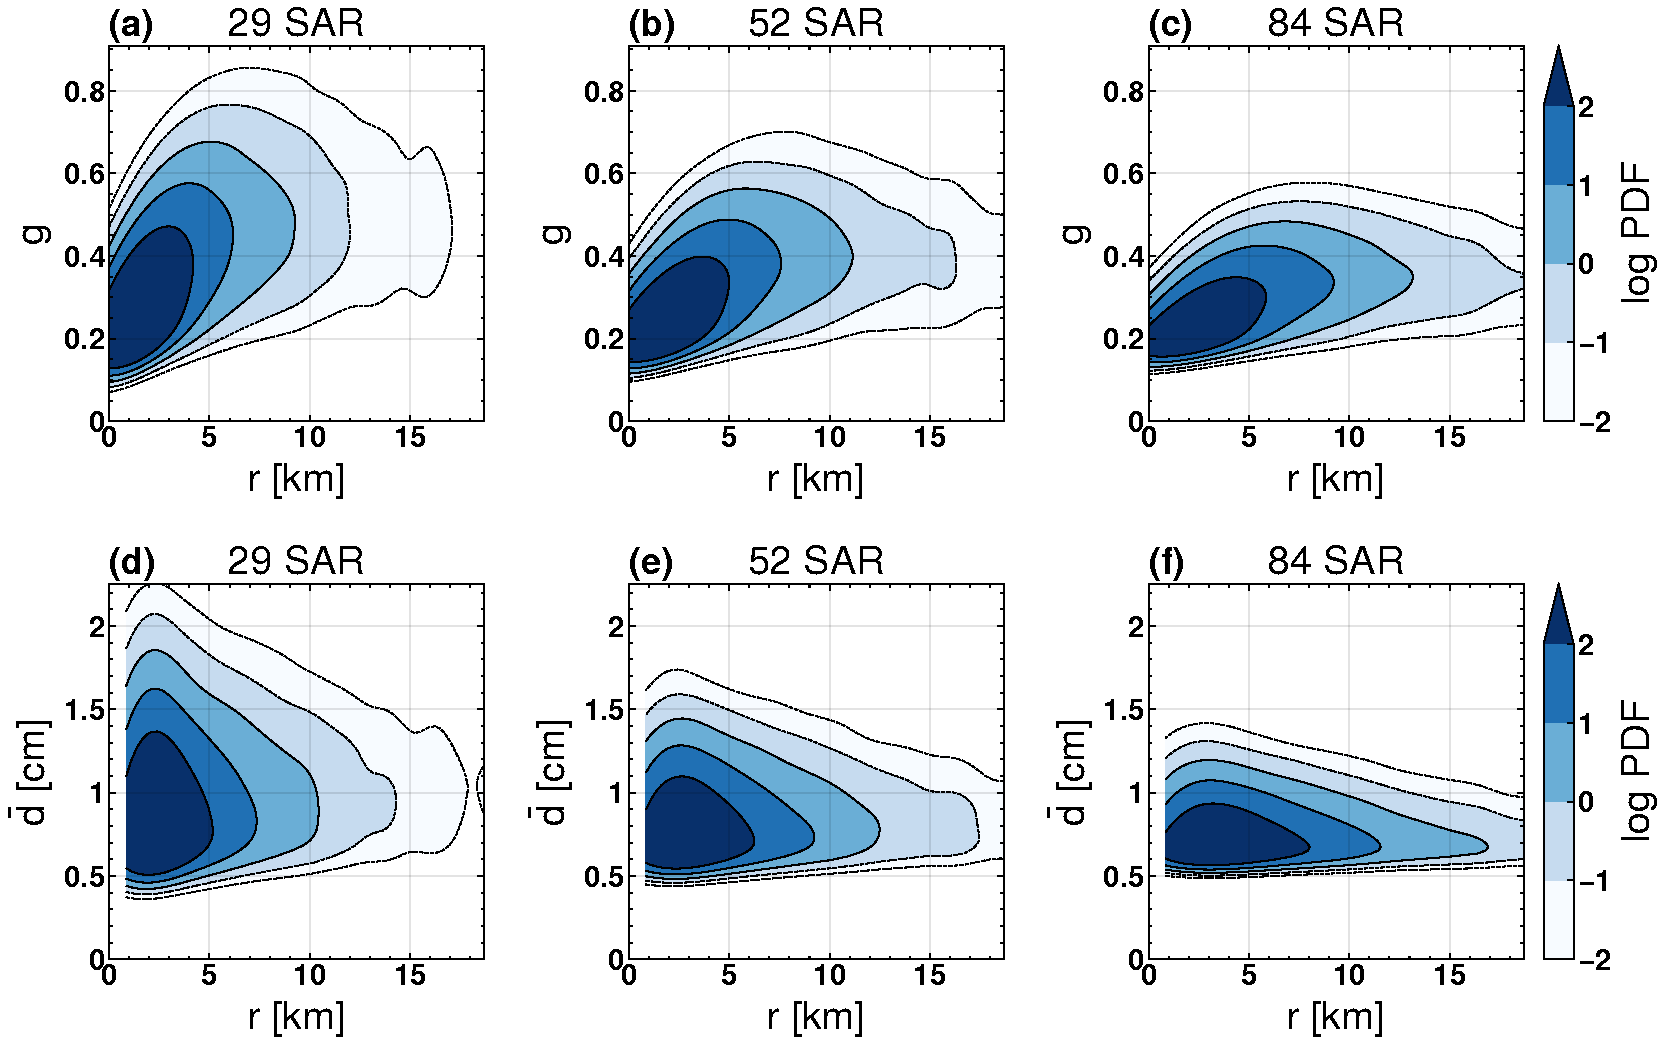
\includegraphics[width=0.98\linewidth]{paper2/figures/figure_results_kde.pdf}
\caption{
Probability of detecting blobs of a given size $r$ and filter magnitude $g$ from tropospheric simulation. Turbulence images were simulated in equal number to the cumulative deformation map using (a) 29 SAR acquisitions, (b) 52 SAR acquisitions, and (c) 84 SAR acquisitions. The detection algorithm was run on each noise-simulated deformation map, and detections tallied into a 2D histogram. The PDF was created from the 2D histogram using a kernel density estimate (KDE) \citep{Scott2015MultivariateDensityEstimation}.
(d-f) Same as top row, but the probabilities were calculated using the image magnitude $|\bar{d}|$.
}
\label{fig:results-kde}
\end{figure*}

%\subsection{West Texas Detected Deformation}

Using the empirical PDFs, we determined the highest probability deformation features contained in the deformation maps derived from Sentinel-1 InSAR (Figure \ref{fig:results-detections}). For the deformation spanning Nov. 2014 - Jan. 2017 (Figure \ref{fig:results-detections}a) using 29 SAR acquisitions. 
We kept detections that have $ > $95\% confidence for the given radius in both the filter magnitude PDF (Figure \ref{fig:results-kde}a) and the image magnitude PDF (Figure \ref{fig:results-kde}d).
We found 57 deformation features ranging from $\sim$1 km to 20 km in radius. This number increases to 147 features through Jan. 2018 (Figure \ref{fig:results-detections}b) and 268 features through Jan. 2019 (Figure \ref{fig:results-detections}c). Note that the increasing number of detections is due to a larger number of SAR acquisitions, which mitigates the noise and increases confidence, and also due to an increasing rate of deformation coinciding with peak oil production \citep{Staniewicz2020InsarRevealsComplex}.

The detected features are clustered into areas within the Midland Basin to the east and the Delaware Basin to the west, with little to no deformation features in the Central Basin Platform. In the Midland Basin, oil production has led to many small (~3-5 km) subsidence bowls with amplitudes of 1-4 cm and areas of 1-3 cm of uplift due to wastewater injection.
Similarly, in the central and northern sections of the Delaware Basin, oil production has created several $\sim10$ km-wide subsidence bowl with amplitudes of 4-8 cm. In the southern portion of the Delaware Basin, linear features resulting from the cluster of earthquakes are detected with high confidence  in the most recent deformation map.


\begin{figure*}[hbt!]
\centering 
%\includegraphics[width=0.98\linewidth]{paper2/figures/figure_results_detections_vert.png}
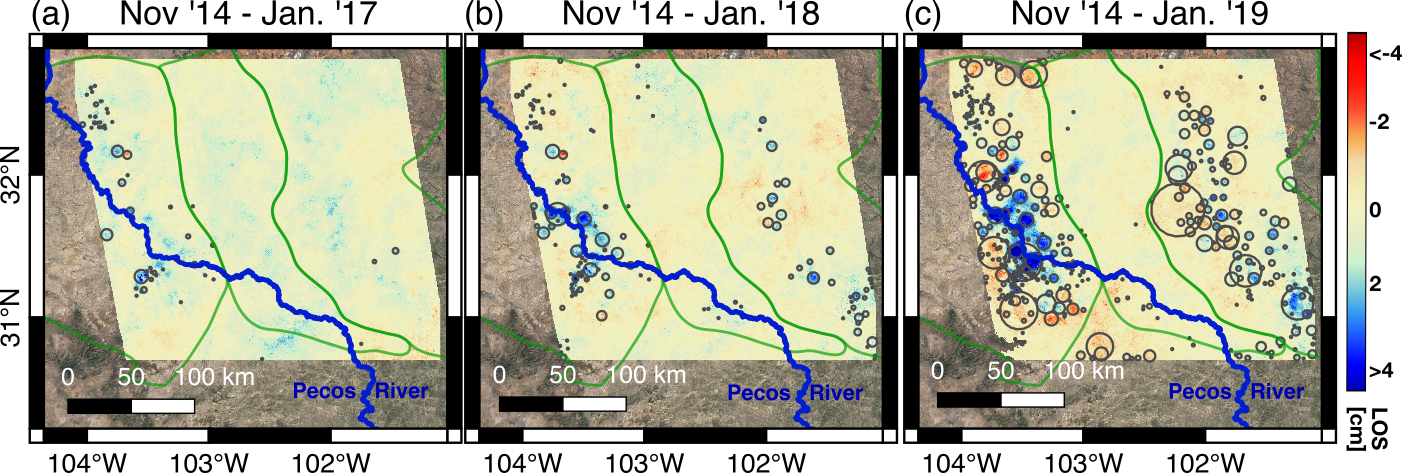
\includegraphics[width=0.98\linewidth]{paper2/figures/figure_results_blobs_path78.png}
\caption{
Detections for ascending path 78 with $ > $95\% confidence for the cumulative deformation from (a) Nov. 2014 - Jan 2017, using 29 SAR acquisitions, (b) Nov. 2014 - Jan 2018, using 52 SAR acquisitions,  (c) Nov. 2014 - Jan 2019, using 84 SAR acquisitions. Red indicates ground deformation toward the satellite (uplift or west), blue indicates motion away from the satellite. More detections are found as time goes on due to 1) a greater number of SAR acquisitions for stacking, leading to greater detection confidence, and 2) increased oil production and wastewater injection, lead to more subsidence and uplift. 
Dark outlined shapes from west to east show locations of the Delaware Basin, Central Basin Platform, and Midland Basin.
}
\label{fig:results-detections}
\end{figure*}



\section{Discussion}
\label{sec:discussion}



\subsection{Effects of Residual Deformation on Spectrum and Simulations}
\label{subsec:discussion-residual-deformation}
We find that the residual deformation term $  \frac{1}{N-1}  \sum  \Delta d_{n,k} $ in Equation \eqref{eq:avg-ifg} does not significantly affect our simulated noise. We demonstrate this by comparing the 1D PSD of a noise estimate on a quiet atmospheric date (2018-09-04, Figure \ref{fig:discussion-residual-defo}a) to the PSD of the sum of the noise and the total cumulative deformation from Nov. 2014 - Jan. 2019 (Figure \ref{fig:discussion-residual-defo}b). When we estimate the PSD after adding the cumulative deformation, the resulting PSD is only slightly larger (Figure \ref{fig:discussion-residual-defo}c). This is because the total integrated power of the noise image is 3.5 cm$^2 $, while the total power of the deformation image is only 20\% of this (0.7 cm$^2 $). Since the residual deformation contribution in Equation \eqref{eq:avg-ifg}, $ \frac{1}{N-1}  \sum  \Delta d_{n,k} $, is much less than the total cumulative deformation, we conclude that this term in the tropospheric noise estimates has negligible effects on the ultimate detection confidences resulting from the simulations.

\begin{figure*}[hbt!]
\centering 
% vertical version:
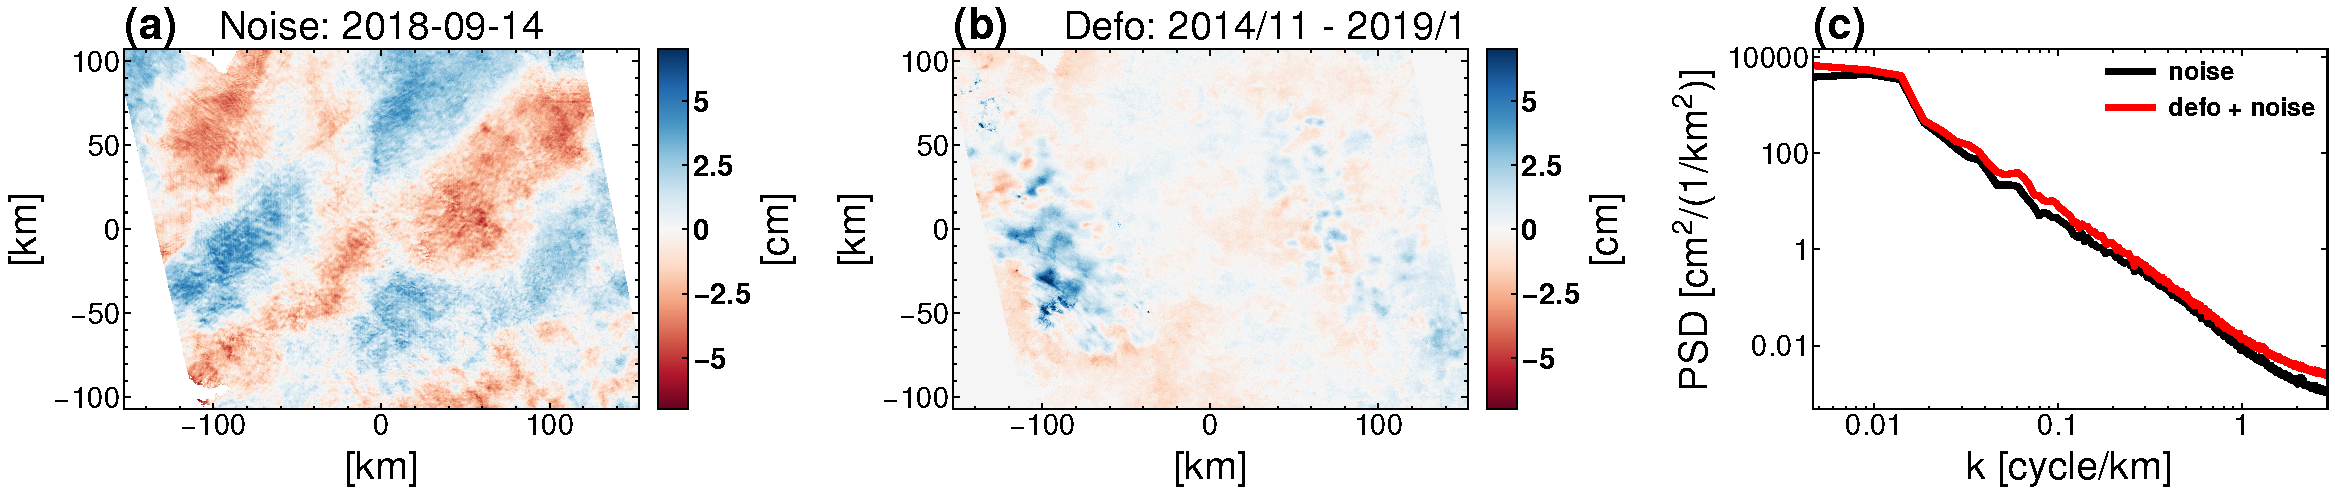
\includegraphics[width=0.98\linewidth]{paper2/figures/figure_discussion_residual_defo.pdf}
%\includegraphics[width=0.98\linewidth]{paper2/figures/figure_discussion_residual_defo_horizontal.pdf}
\caption{
(a) Estimated tropospheric noise of path 78 SAR acquisition on 2018-09-14. 
(b) Cumulative LOS deformation of path 78 from Nov. 2014 to Jan. 2019.
(c) 1D PSD of panel (a) (black), and 1D PSD of panels (a) and (b) (red) .
}
\label{fig:discussion-residual-defo}
\end{figure*}


\subsection{Comparison to Path 85 Detections}
\label{subsec:discussion-path85}

Due to the differences in acquisition times (7:50 p.m. local time for path 78, 6:55 a.m. for path 85), the turbulence is milder on average for path 85 (Figure \ref{fig:discussion-noise-85}). Similar to path 78 (shown in Figure \ref{fig:results-noise}(d)), approximately 50\% of SAR acquisitions have quiet atmospheric conditions with a peak noise level under 4 cm (Figure \ref{fig:discussion-noise-85}a). However, there are only two path 85 acquisitions with over 10 cm of peak noise, compared to 14 acquisitions for path 78. The difference in noise level is also apparent in the growth of RMS noise vs. distance to the reference point (Figure \ref{fig:discussion-noise-85}b). While the shape of the growth is similar for ascending and descending, the ascending path 78 has 50\% larger average noise at 50 km from the reference. Similarly, the average PSDs for path 78 and path 85 have similar shape (Figure \ref{fig:discussion-noise-85}b), but the mean power for path 78 is over 2 times larger at a spatial frequency of 0.1 cycles/km. We summarized the noise statistical differences by comparing 1) the mean variance of each noise map, 2) the largest variance of any map, 3) the mean peak amplitude of the noise map, and 4) the largest peak across all dates (Table \ref{tab:path85-compare}).




\begin{figure*}[hbt!]
\centering 
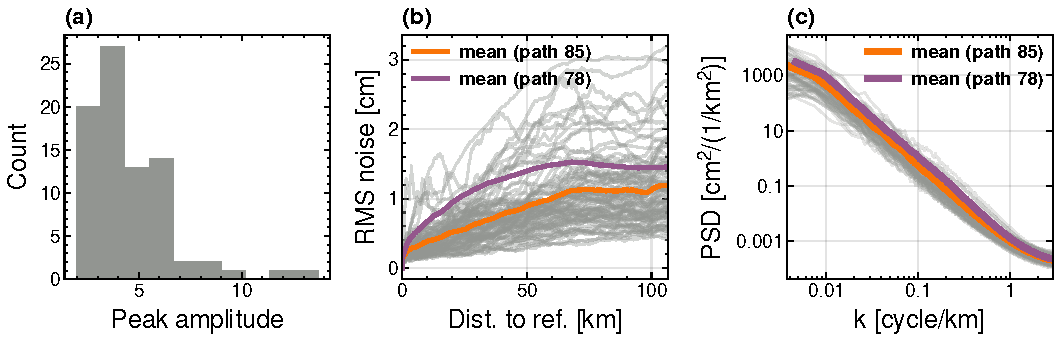
\includegraphics[width=0.98\linewidth]{paper2/figures/figure_discussion_path85_plots.pdf}
\caption{
(a) Histogram of peak absolute value for 81 estimated noise maps from path 85. 
(b) Root mean squared value of noise vs distance from reference point for path 85 estimated noise maps (gray lines). The mean of these lines (orange) is plotted for comparison with the mean of path 78 (purple).
(c) 1D PSDs for 81 SAR acquisitions from path 85 (gray lines). The mean of path 85 (orange) smaller than the mean of path 78 (purple). 
}
\label{fig:discussion-noise-85}
\end{figure*}


\begin{table}
\centering
\caption{Summary of noise differences between path 85 and path 78}
\begin{tabular}{lrr}
\toprule
{} &  Path 78 &  Path 85 \\
\midrule
Average Variance [cm$^2$]             &     1.38 &     0.78 \\
Variance of Noisiest Date [cm$^2$] &    10.68 &     3.74 \\
Average Peak Amplitude [cm]            &     5.36 &     4.58 \\
Largest Peak Amplitude [cm]         &    15.81 &    13.72 \\
%\midrule
%Detected features with confidence $p<0.05$ & & \\
%\midrule
%Through Jan '17 & 48 & 58 \\
%Through Jan '18 & 102 & 130 \\
%Through Jan '19 & 256 & 343 \\
\bottomrule
\end{tabular}
\label{tab:path85-compare}
\end{table}




Due to the lower noise of path 85, there are more detected features at a confidence level of p $< 0.05 $ (Figure \ref{fig:discussion-detections-85}). Our algorithm found similar numbers of total deformation candidates in path 78 and path 85 (between 1000-1500 per year); most of these candidates are faint noise artifacts and given a low confidence score. However, the smaller average tropospheric noise in path 85 means that the same feature will scored more confidently as a real deformation signal in path 85 than in path 78.  For example, while both path 78 and path 85 detect the significant deformation in the Delaware Basin due to oil production, there are several detections with magnitude $\sim1$cm in the path 85 image near wasterwater injection wells in the Central Basin Platform. 

It is also worth noting that both paths show a large increase in the number of detections from 2016 though the end of 2018, coinciding with the overall rise in oil production within the Permian Basin (Figure \ref{fig:discussion-oil-blob-count}). While some of the increase in high confidence detections is due to the availability of more SAR acquisitions, the total oil production in the Permian Basin increase  $>60\%$, from an average daily production of 1.5 Mbbl / day in 2016 to 2.5 Mbbl / day in 2018. This led to a large number of subsidence and uplift bowls detected in the Midland and Delaware Basins.



\begin{figure*}[hbt!]
\centering 
%\includegraphics[width=0.98\linewidth]{paper2/figures/figure_discussion_blobs_path85.png}
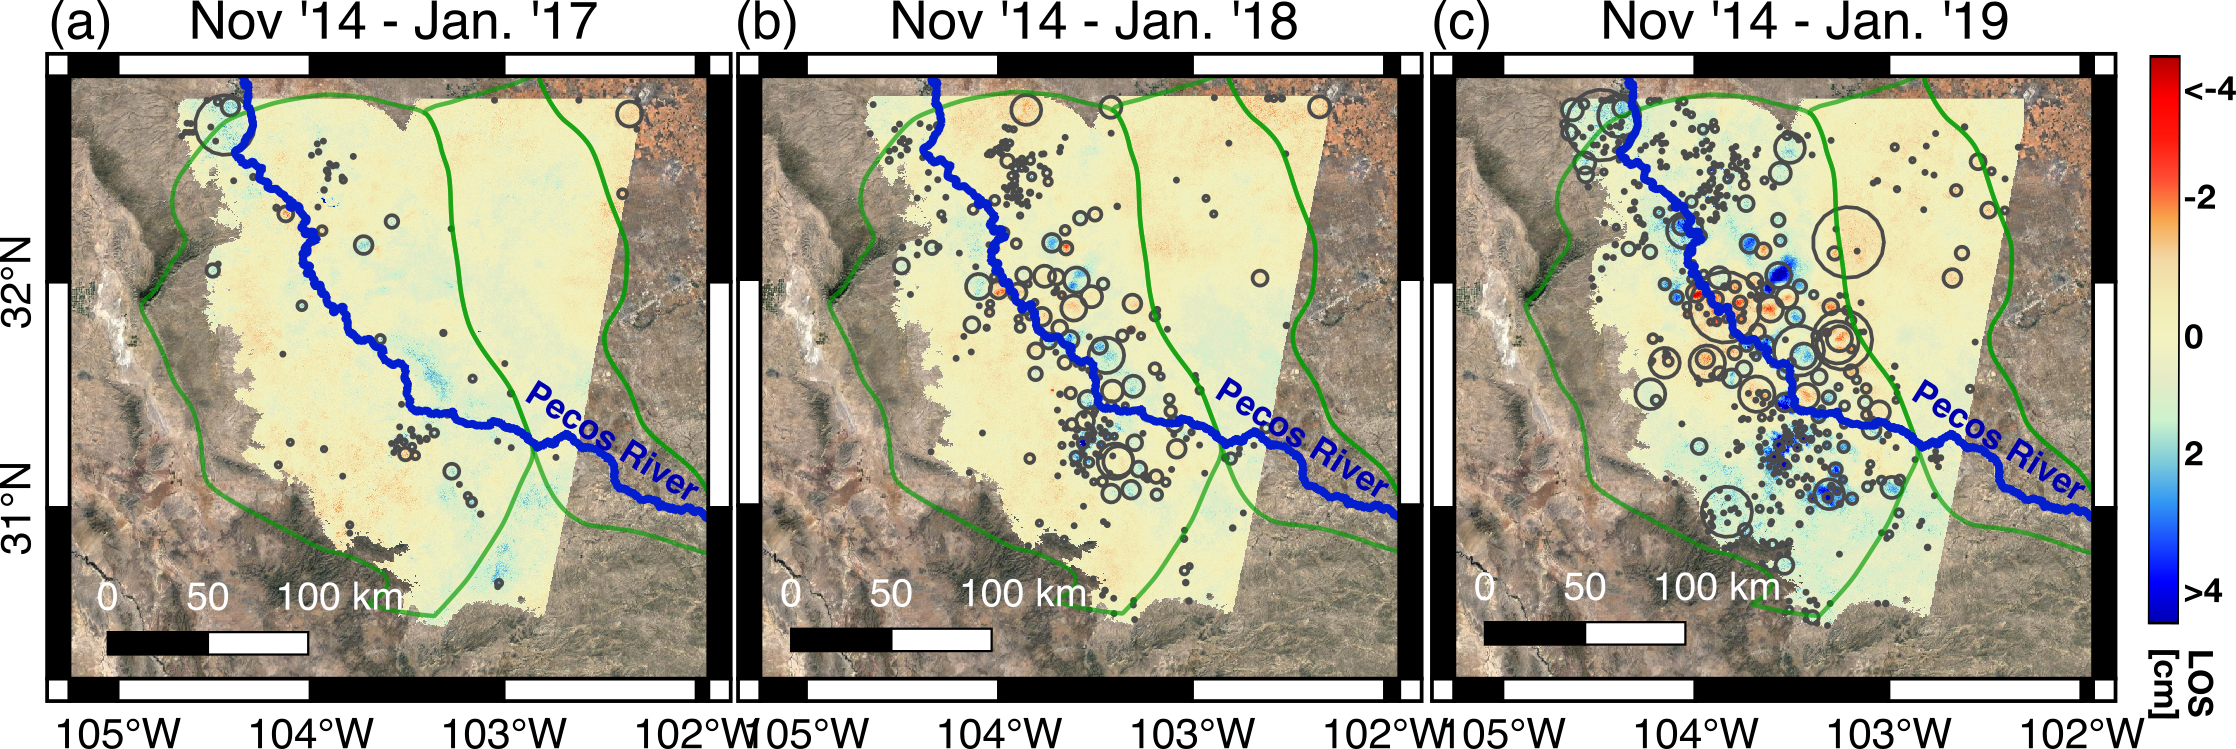
\includegraphics[width=0.98\linewidth]{paper2/figures/figure_discussion_blobs_combined_path85.png}
\caption{
Detections for descending path 85 with $ > $95\% confidence for the cumulative deformation from (a) Nov. 2014 - Jan 2017, using 27 SAR acquisitions, (b) Nov. 2014 - Jan 2018, using 55 SAR acquisitions,  (c) Nov. 2014 - Jan 2019, using 81 SAR acquisitions. Red indicates ground deformation toward the satellite (uplift or east), blue indicates motion away from the satellite. Dark outlines show location of the Delaware Basin (center) and the Central Basin Platform (to the east).
}
\label{fig:discussion-detections-85}
\end{figure*}


\begin{figure}[hbt!]
\centering 
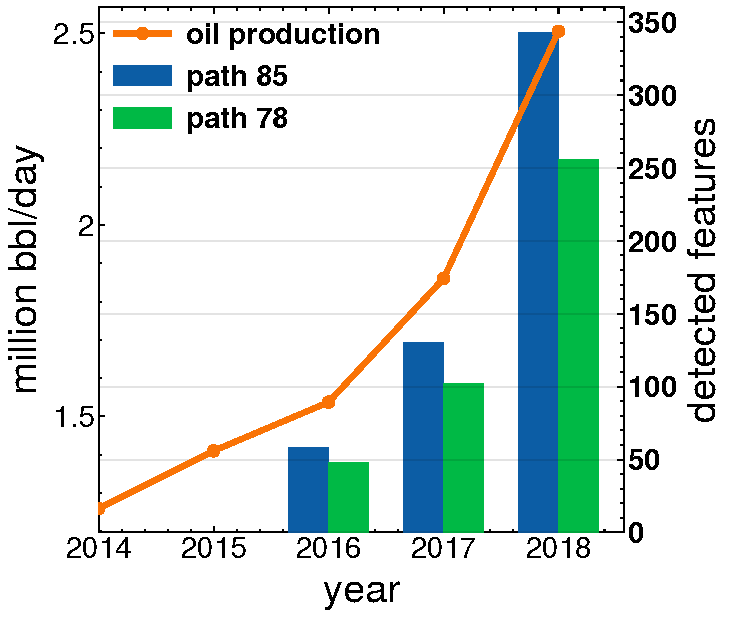
\includegraphics[width=0.98\linewidth]{paper2/figures/figure_discussion_oil_vs_blob_count.pdf}
\caption{
The average daily oil production for the Permian Basin for the years 2014-2018 (orange), along with the number of detected deformation features for path 85 (blue) and path 78 (green).
}
\label{fig:discussion-oil-blob-count}
\end{figure}

\subsubsection{Radial average vs 1D line}

If a 2D random field $\phi(x, y)$ has Fourier transform $\Phi(k_x, k_x)$, we can express the field in the spatial domain in terms of its frequency domain representation:
\begin{gather}
    \phi(x, y) =  \int_{-\infty}^{\infty} \int_{-\infty}^{\infty} \Phi(k_x, k_y) e ^{j 2 \pi (\bm{x} \cdot \bm{k}) } \, d k_x \,d k_y \\
   \phi(r, \theta) = \int_{-\infty}^{\infty} \int_{-\infty}^{\infty} \Phi(r_k, \theta_k) e ^{j 2 \pi (r r_k \cos \theta_k ) } r_k \, d r_k \,d \theta_k
\end{gather}
where $\bm{x} = [x \quad y]^T$ and $\bm{k} = [k_x \quad k_y]^T$, $r = \sqrt{x^2 + y^2}$,  $r_k = \sqrt{k_x^2 + k_y^2}$, $\theta = \arctan \frac{y}{x}$, and $\theta_k = \arctan \frac{k_y}{k_x}$.

If we assume the field $\Phi(k_x, k_y)$ is isotropic and radially symmetric, it is only a function or $r$, so $\Phi(r_k, \theta_k) = \Phi(r_k) $.

....TODO...

If the power spectrum is a power law, $\Phi(r_k) = C \frac{1}{r_k}^\beta$. 



\subsection{Conclusions}


\chapter{Conclusions}


\appendix



\section{ Dislocation (Fault Slip) Model}
\cite{Okada1992InternalDeformationDue} derived the analytical surface displacement field due to a finite rectangular fault slip in an elastic half-space. The Okada solutions provide three cases of displacement on a fault: strike-slip, dip-slip, tensile opening. In this study, we focused on the dip-slip case, because the Pecos area is in a normal faulting regime \cite{LundSnee2018}.  The assumption of predominant dip-slip along normal faults is also supported by fault plane solutions (TexNet Earthquake Catalog). 

Considering the case of dip slip on a finite rectangular fault (Figure \ref{fig:model-fault-geom}), the vertical surface displacement $u_z(x, y, 0)$ can be expressed as:
\begin{equation}
	u_{z}(x,y,0)=\frac{U_{2}}{2\pi }[u_{2}^{B}\sin \delta + u_{3}^{B}\cos \delta]
	\label{eq:okada}
\end{equation}
where $U_2$ is the magnitude of dip slip. The rest of terms on the right are determined by fault geometry parameters: the fault dip angle ($\delta$), the depth to the top of the fault ($Z$), the fault width along the dip direction ($W$), and the fault length along the strike direction ($L$). 

We located four faults based on InSAR observations, and assumed a uniform slip on each fault. We estimated the best-fit fault parameters for each fault independently by minimizing the objective function \cite{Du1992}:
\begin{equation}
	\arg \min_{U_{2,i}} \left \| \mathbf{G_i}U_{2,i}-\mathbf{d_i} \right \|^2_{2}  
	\label{eq:model-obj-1}
\end{equation}	  	
where $\mathbf{G_i}$ is the discrete Green’s function that maps a dip slip, $U_{2,i}$, on the $i^{th}$ rectangular fault to the observed vertical deformation at specific surface locations.  $\mathbf{G_i}$ is a function of fault geometry parameters as shown in Equation \eqref{eq:okada}. $\mathbf{d_i}$ is a vector of vertical deformation observations associated with the $i^{th}$ fault from InSAR data.

Through a grid-search, we solved for the fault dip angle, the depth to the top of the fault, the width along the dip direction, and the magnitude of dip slip on each fault to minimize the sum of squared residuals normalized by the data error of 1 cm (Normalized Sum of Squared Residuals; NSSR). The fault length in the strike direction is set to be sufficiently long to satisfy the plane strain condition. As an example, Figure \ref{fig:fault-supplement-nssr} shows how the data misfit varies with fault parameters for fault \#3. The maximum R-squared ($R^2$) values for the best-fit fault parameters are in the range of 0.95 and generally agree with the fault parameters that satisfy the minimum NSSR. 

The best-fit fault parameters of the four faults are listed in Table \ref{tab:geo-mech-fault}, which produce 3D surface deformation patterns as shown in Figure \ref{fig:fault-model-xyz}. To illustrate how surface deformation observations are related to the model parameters, Figure \ref{fig:fault-supplement2} shows the estimated surface subsidence associated with the fault \#3 long the B-B' transect with various fault properties. The ratio of the uplift volume to the subsidence volume is a function of the seismic potency and the fault dip angle \cite{Segall2019integrated}. Based on the results in Figure \ref{fig:fault-supplement2} (a), the fault dip angle dominantly controls the uplift volume relative to the subsidence volume. The slope from the uplift on the footwall to the subsidence on the hanging wall becomes steeper as the fault becomes shallower (Figure \ref{fig:fault-supplement2} (b)). The fault width, as measured along the the dip direction, mostly contributes to the width of the subsidence bowl (Figure \ref{fig:fault-supplement2} (c)).  The dip-slip magnitude only has impact on the amplitude of the curve without any influence on the shape of the surface deformation (Figure \ref{fig:fault-supplement2} (d)).




\begin{figure}
	\centering
	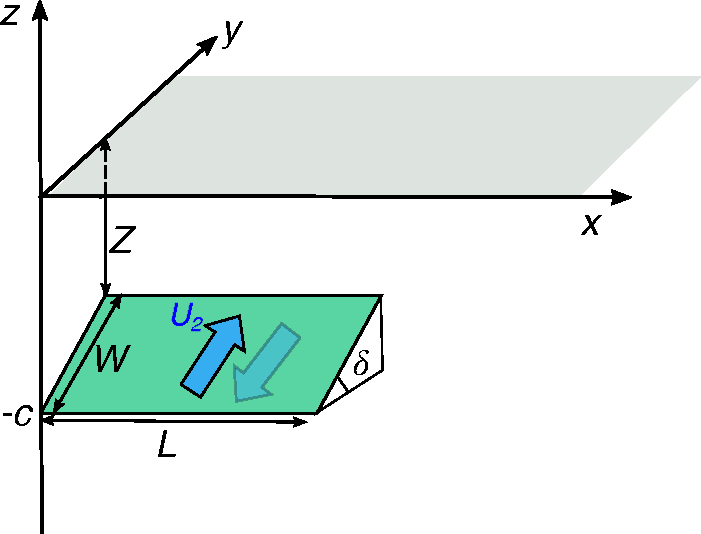
\includegraphics[width=\textwidth]{paper1-permian/figures/supplement/figureS6-fault-geom.pdf}
	\caption{A finite rectangular fault model \cite{Okada1992}. Here $U_2$ is the magnitude of dip slip (positive in reverse fault direction), $\delta$ is the dip angle, $Z$ is the depth to the top of the fault, $c$ is the depth to the bottom of the fault, $L$ is the length along the strike direction, and $W$ is the width along the dip direction.}
	\label{fig:model-fault-geom}
\end{figure}

\begin{table}
	\centering
	\caption{Best-fit fault parameters as derived from the dislocation model}
	\begin{tabular}{c|cccc}
		& Fault \#1      & Fault \#2      & Fault \#3      & Fault \#4      \\
		\hline
		1-Longitude ($^{\circ}$) & -103.563 & -103.589 & -103.585 & -103.529 \\
		1-Latitude ($^{\circ}$)  & 31.367   & 31.413   & 31.463   & 31.470   \\
		2-Longitude ($^{\circ}$) & -103.503 & -103.505 & -103.440 & -103.468 \\
		2-Latitude ($^{\circ}$)  & 31.337   & 31.355    & 31.374   & 31.432   \\
		Dip Angle ($^{\circ}$)   & 60       & 60       & 50       & 57.5       \\
		Depth (km)               & 0.91     & 0.91     & 1.07     & 1.52     \\
		Width (km)              & 0.61     & 0.30     & 1.07     & 0.61     \\
		Slip (cm)                & 9.1     & 15.2     & 9.1     & 15.2    \\
	\end{tabular}
	\label{tab:geo-mech-fault}
\end{table}

\begin{figure}
	\centering
	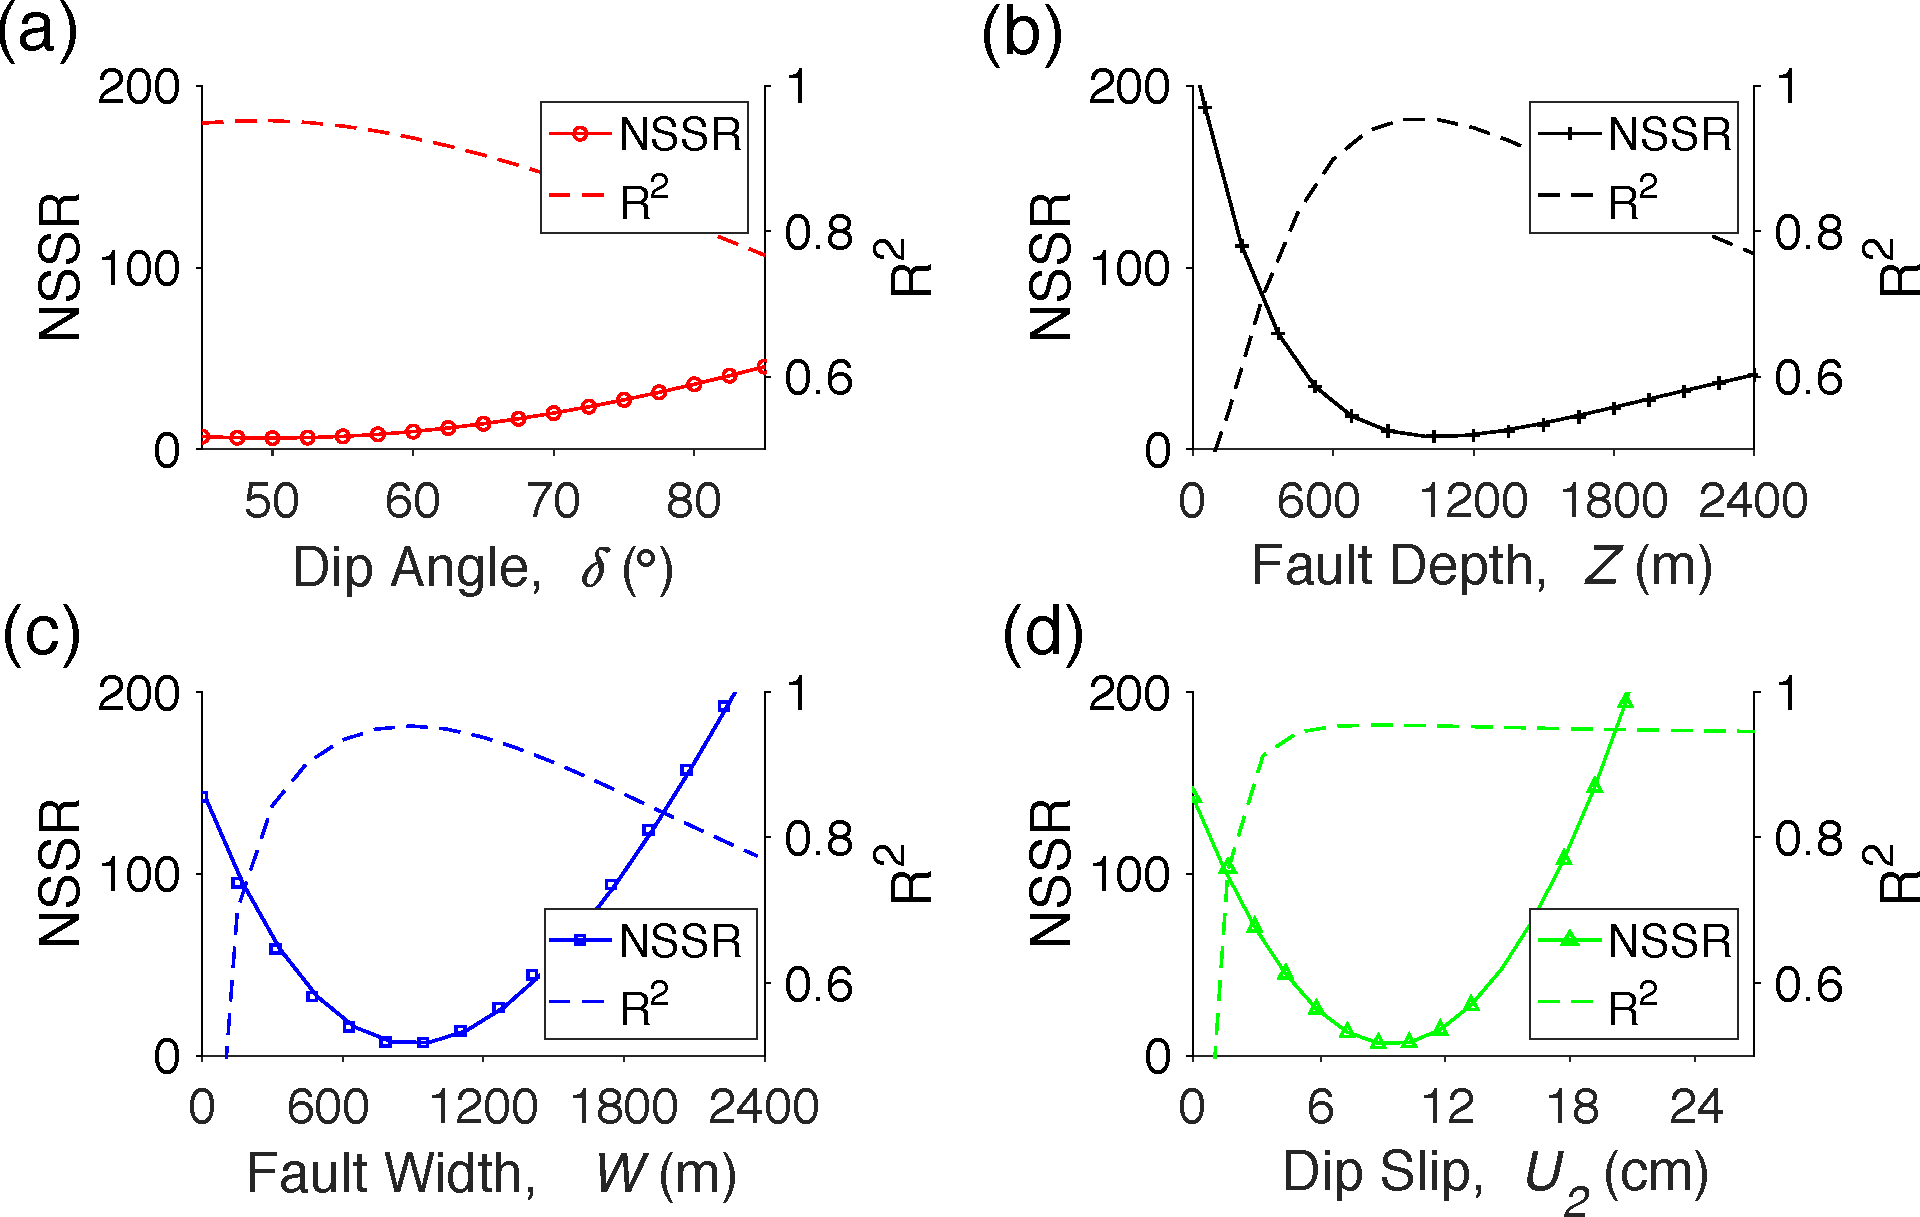
\includegraphics[width=.98\textwidth]{paper1-permian/figures/supplement/figureS7-fault-supplement-nssr.pdf}
	\caption{The Normalized Sum of Squared Residuals (NSSR) and R-squared ($ R^2 $) of fault \#3 relative to (a) fault dip angle ($ \delta $), (b) fault depth from the surface to the top of the fault ($ Z $), (c) fault width along the dip direction ($ W $), and (d) net dip slip magnitude ($ U_2 $).}
	\label{fig:fault-supplement-nssr}
\end{figure}

\begin{figure}
	\centering
	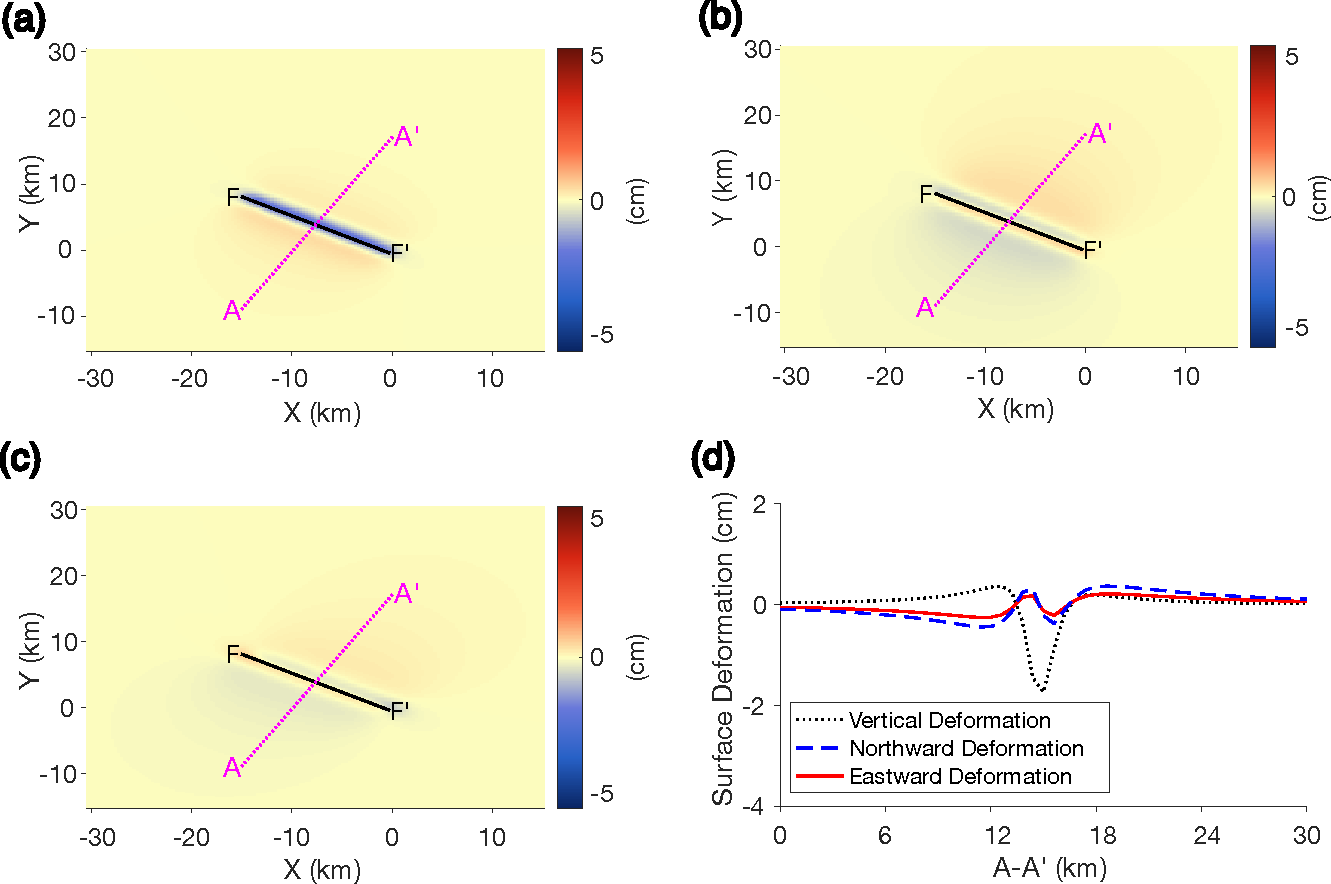
\includegraphics[width=\textwidth]{paper1-permian/figures/supplement/figureS8-fault-predicted-xyz.pdf}
	\caption{The predicted surface deformation from the Okada fault model with best-fit parameters in the (a) vertical direction (positive means uplift), (b) northward direction (positive means north, negative means south), and (c) eastward direction (positive means east, negative means west). (d) Comparison of the 3D deformation profiles along A-A$^{'} $ transect that is perpendicular to fault plane.
	}
	\label{fig:fault-model-xyz}
\end{figure}

\begin{figure}
	\centering
	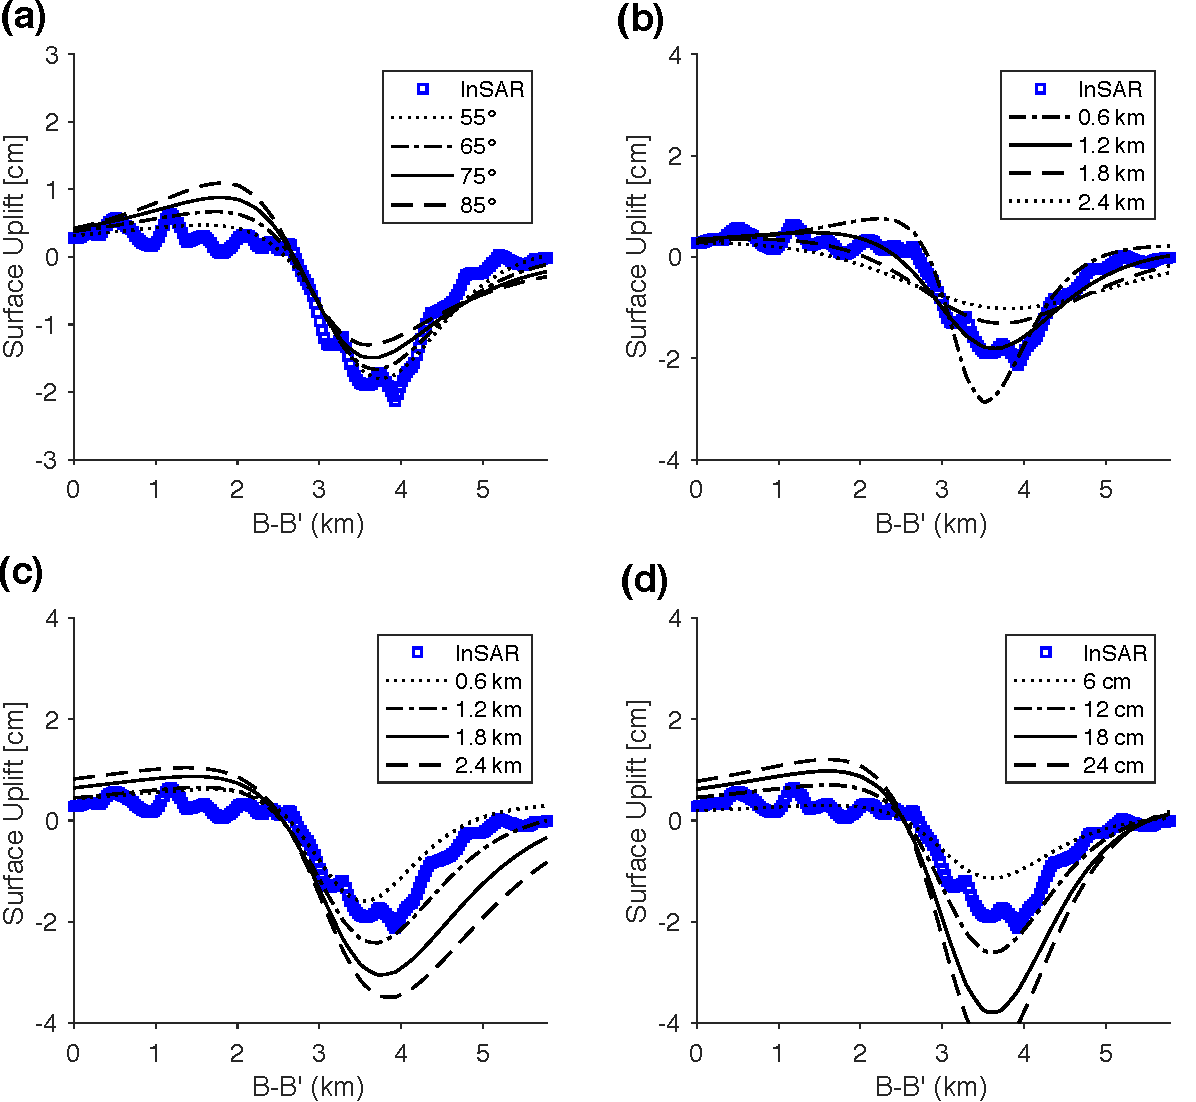
\includegraphics[width=\textwidth]{paper1-permian/figures/supplement/figureS9-fault-supplement2.pdf}
	\caption{Estimated surface subsidence along the B-B' transect associated with fault \#3 with various fault properties: (a) fault dip angle ($ \delta $) of 55$ ^{\circ} $, 65$ ^{\circ} $, 75$ ^{\circ} $, 85$ ^{\circ} $, (b) fault depth from the surface to the top of the fault ($ Z $) of 0.6 km, 1.2 km, 1.8 km, 2.4 km, (c) fault width along the dip direction, $ W $) of 0.6 km, 1.2 km, 1.8 km, 2.4 km, and (d) net dip slip magnitude ($ U_2 $) of 6 cm, 12 cm, 18 cm, 24 cm.}
	\label{fig:fault-supplement2}
\end{figure}


\pagebreak

\section{ Cylindrical Reservoir Compaction/Subsidence Model}
\label{sec:model-compact}
\cite{Geertsma1973LandSubsidenceCompacting} derived the surface displacement field due to a uniform pressure drop of a cylindrical reservoir at a depth $D$ (Figure \ref{fig:model-reservoir-geom}). Under the assumption that the reservoir radius $R$ is larger than the reservoir height $H$, the cylindrical reservoir deforms primarily in the vertical direction. The magnitude of the reservoir compaction $\Delta H$ due to a pressure drop $\Delta P$ can be written as:
\begin{equation}
	\Delta H = H c_m \Delta P
	\label{eq:rcompact}
\end{equation}
Here the  uniaxial compaction coefficient $c_m$ can be expressed as
\begin{align}
	c_{m} &= \alpha_{p}\frac{1+\nu}{1-\nu}\frac{c_{b}}{3} 
\end{align}
where $\alpha_p$ is Biot's coefficient, $c_b$ is the bulk compressibility, and $\nu$ is the Poisson's ratio. Surface vertical deformation $u_z$ due to the reservoir compaction $\Delta H$ can be expressed as:
\begin{align}
	u_{z}(r,0) &= 2(1-\nu)\Delta HA(\rho,\eta) 
	\label{eq:reservoirDef}
\end{align}
where $ A(\rho,\eta) = R\int_{0}^{\infty}e^{-D\alpha}J_{1}(\alpha R)J_{0}(\alpha r) \, d\alpha$, $\rho = r/R$, and $\eta =  D/R$. The maximum surface deformation at $r = 0$ can be written as:
\begin{equation}
	{u_{z}}^{max} = 2(1-\nu)\Delta H(1-\frac{\eta}{\sqrt{1+\eta^{2}}})
\end{equation}

The best-fit compaction in the cylindrical reservoirs were determined by minimizing the objective function \cite{Du2001}:
\begin{equation}
	\arg \min_{\mathbf{\Delta H}} =\left \| \mathbf{G_R}\mathbf{\Delta H}-\mathbf{d_r} \right \|^2+\beta ^2\left \| \mathbf{H_L}\mathbf{\Delta H}-\mathbf{d_0} \right \|^2  \label{eq:model-obj-2}
\end{equation}
where $ \mathbf{G_R} $ is the discrete Green’s function that maps the compaction of cylindrical reservoirs $\mathbf{\Delta H}$ in the subsurface to the observed vertical deformation at specific surface locations. $\mathbf{G_R}$ is a function of reservoir geometry parameters as shown in Equation \eqref{eq:reservoirDef}. $\mathbf{d_r}$ is a vector of vertical deformation observations associated with the reservoir compaction. In this study, $\mathbf{d_r}$ is the difference between the InSAR-observed total vertical deformation and modeled vertical fault slip deformation, $ \beta^2 $ is the penalty factor that weights the smoothness constraint, and $ \mathbf{H_L} $ is the finite difference approximation of the Laplacian operator. The reservoir compaction is constrained to be negative, and $\mathbf{d_0} $ is set to be zero. 

Based on the production well data near Pecos, we discretized two layers of reservoirs in the subsurface: Delaware Mountain Group (DMG) at depth 1.52 km and Wolfcamp at depth 3.05 km (Figure \ref{fig:model-reservoir-wells}). The shallow groundwater level reservoirs were not included in the reservoir model, because the water levels in the groundwater aquifers in the Pecos area were stable over the time period of interest \cite{deng2020surface}. The producing wells in the DMG were predominantly located to the east of Pecos, and we set 25 cylindrical reservoirs with the radius of 0.83 km. In the Wolfcamp formation, the wells were producing over the entire region. We discretized the layer covering the entire area with 100 cylindrical reservoirs with the radius of 0.83 km.  

We utilized the pattern search optimization tool in MATLAB to minimize the objective function (Equation \eqref{eq:model-obj-2}). As the penalty factor $\beta^2$ decreases, the NSSR decreases, $ R^2 $ increases, and the modeled surface deformation better matches the InSAR data (Figure \ref{fig:model-reservoir-nssr}). Once the penalty factor ($ \beta^2 $) is smaller than 0.01, the NSSR and $ R^2 $ no longer change substantially. The best-fit reservoir compaction results ($ \beta^2 $ equals 0.01) for the two producing layers are shown in Figure \ref{fig:model-reservoir-wells}. While DMG reservoirs show some compaction (0 - 8 cm), the dominant compaction is in the Wolfcamp layer (0 - 27 cm). The production volume in DMG is as significant as in Wolfcamp. However, the dominant injection volume into DMG could maintain the reservoir pressure and minimize reservoir compaction. For certain regions in the Wolfcamp layer, the reservoir compaction appears to be discontinuous given the low $ \beta^2 $ value. We note that it is reasonable to observe localized compaction for tight shale formations, because the low formation permeability can cause heterogeneous pressure distribution during the depletion.

If appropriate mechanical properties of the formation are available, the distribution of reservoir pressure change and depleted zone can be evaluated by the reservoir compaction magnitudes based on Equation \eqref{eq:rcompact}. For example, if we assume Young’s modulus of 25 GPa, Poisson’s ratio of 0.25, and Biot’s coefficient of 0.67 based on published rock properties \cite{Shukla2013, Xu2015analysis}, the localized maximum pressure drop is approximately 21 MPa. This is within a reasonable range given operational history in the area.



\begin{figure}
	\centering
	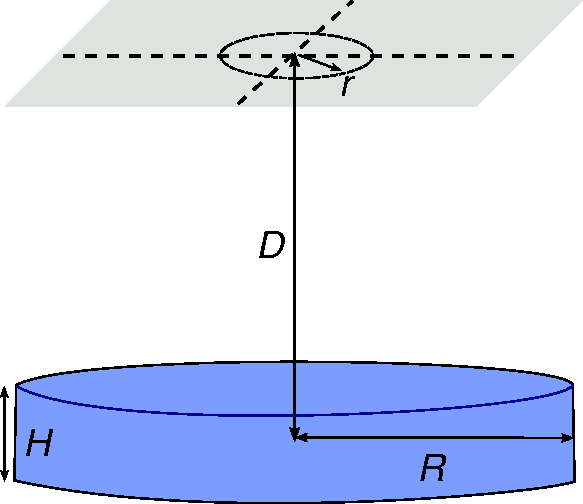
\includegraphics[width=.8\textwidth]{paper1-permian/figures/supplement/figureS10-reservoir-geom.pdf}
	\caption{
		Geometry of reservoir model in \cite{Geertsma1973}, where $H$ is the reservoir height, $D$ is the reservoir depth, and $R$ is the reservoir radius.
	}
	\label{fig:model-reservoir-geom}
\end{figure}

\begin{figure}
	\centering
	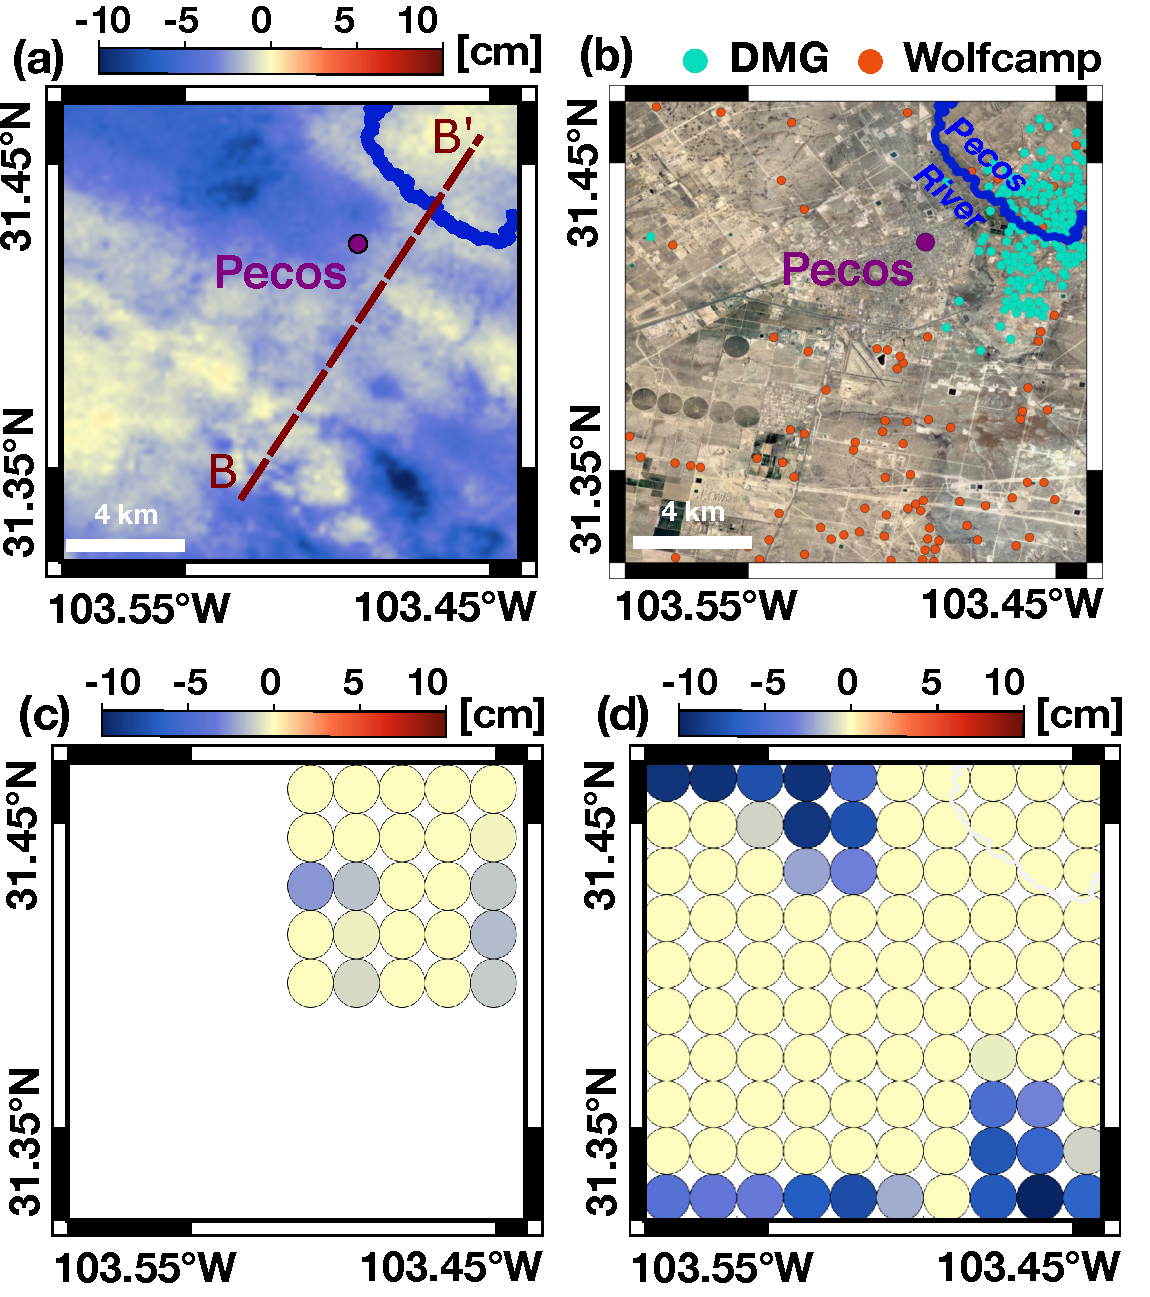
\includegraphics[width=\textwidth]{paper1-permian/figures/supplement/figureS11-reservoir-wells.pdf}
	\caption{(a) Input for reservoir model: vertical surface deformation difference between InSAR and fault model (vertical surface deformation not explained by the fault model). (b) Producing well locations in near Pecos in the Delaware Mountain Group (DMG, cyan) and Wolfcamp (orange). Reservoir compaction values in (c) DMG reservoirs at depth 1.52km, and (d) Wolfcamp reservoirs at depth 3.05km. 
	}
	\label{fig:model-reservoir-wells}
\end{figure}


\begin{figure}
	\centering
	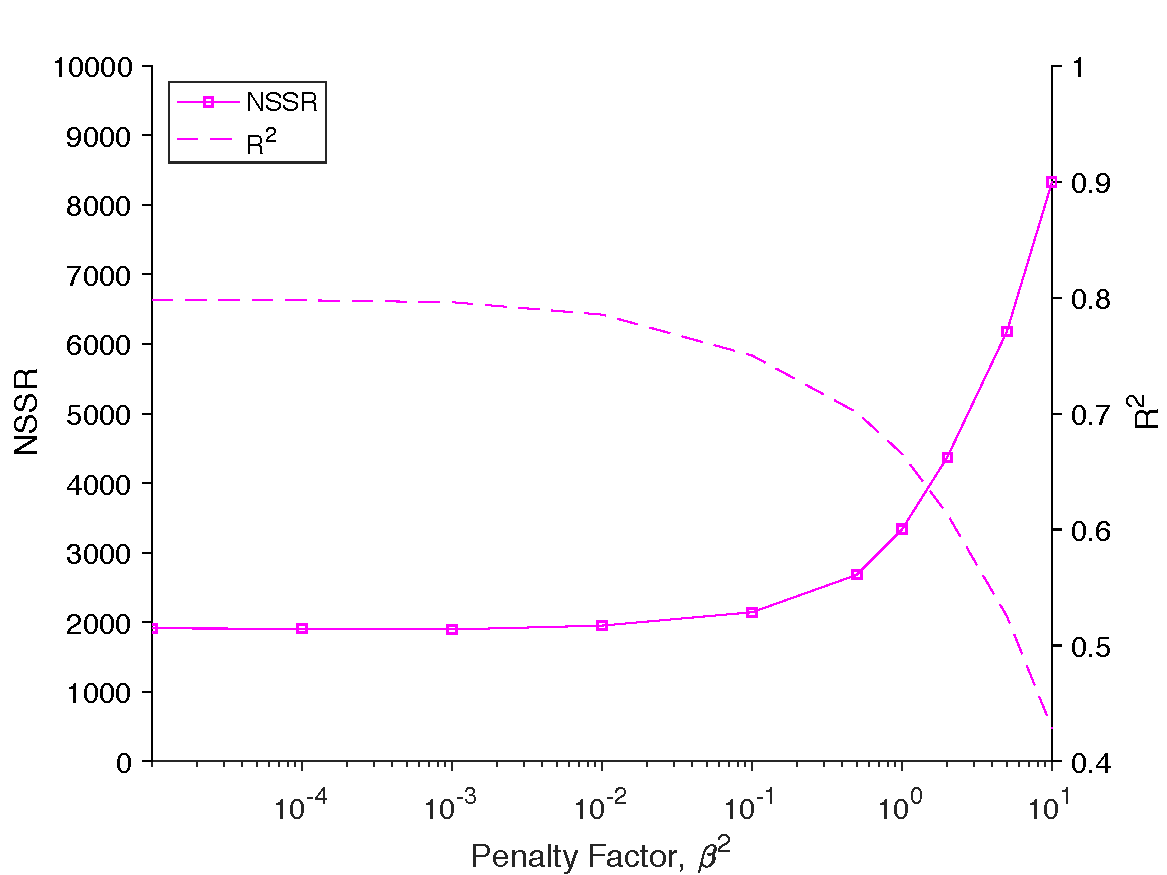
\includegraphics[width=\textwidth]{paper1-permian/figures/supplement/figureS12-reservoir-nssr.pdf}
	\caption{The Normalized Sum of Squared Residuals (NSSR) and R-squared ($ R^2 $) with varying penalty factor ($ \beta^2 $) for the discretized reservoir compaction model
	}
	\label{fig:model-reservoir-nssr}
\end{figure}




%\section{Disambiguating terms from fractal surfaces, Gaussian random
%	fields, and power
%	laws}
%\label{disambiguating-terms-from-fractal-surfaces-gaussian-random-fields-and-power-laws}
%
%Part that I wanted to write down:
%
%Another way to consider fractals: If you generate white or pink noise, unlike human speech or music, it will sound the same at any speed.
%
%Note on Brownian motion being an integral of white noise.
%For any complex sinusoid $x(t) = e^{j2 \pi f t}$ of frequency $f$, the effect in the frequency domain can found by noting that 
%
%\begin{equation}
%	\int x(t) \, dt = \frac{1}{j 2 \pi f} e^{j2\pi f t} = \frac{1}{j 2 \pi f} x(t)
%\end{equation}
%
%Since integration is linear and time invariant, we can think of it as an LTI filter $h$ with frequency response $H_i(f) = \frac{1}{j 2 \pi f} $, which has a $|1/f|$ magnitude response, or $|1/f^2|$ in power.
%
%A white noise process $w(t)$ can be defined as having a flat power spectral density (PSD) $S_W(f) = \sigma^2$. Integrating white noise results in the PSD being shaped into $S_W(f) H_i(f) = \sigma / f^2$.
%
%\textbf{Driving question}:
%
%Is the fractal atmospheric surface (a type of spatially correlated
%noise), which has a power-law power spectrum of
%
%\[S(f) = (1/f)^{\beta}\] also a Gaussian random field?
%
%The three related subjects are\ldots{} - Gaussian Fields - Fractal
%surfaces - Power-law power spectra Can all three be present? Or are some
%mutually exclusive?
%
%\textbf{POSSIBLE SUMMARY ANSWER}
%
%Yes, the surface can be 1. fractal, since the structure function (aka
%semi-variogram) of the atmospheric delay has a power-law form (Hanssen,
%Eq 4.7.10) \footnote{Hanssen, Ramon F. Radar interferometry: data
%	interpretation and error analysis. Vol. 2. Springer Science \&
%	Business Media, 2001.} :
%
%\[D_s(\rho) \sim \rho^{5/3}\]
%
%\begin{enumerate}
%	
%	\item
%	A Gaussian field, since by (Cressie, 1993) Eq. 5.5.1 \footnote{Cressie,
%		Noel. Statistics for spatial data. John Wiley \& Sons, 2015.},
%\end{enumerate}
%
%More generally, a fractional Brownian motion in \(R^d\) is a Gaussian
%process \(Z(\cdot)\) characterized by a covariance function of the form
%with
%
%\[C(s, t) = \frac{1}{2}\left(s^{2H} + t^{2H} + |s-t|^{2H}\right)\]
%
%and a variogram of the form
%
%\[E[(Z(s + h) - Z(s))^2] \propto ||h||^{2H}\] So, for the Hanssen
%structure fucntion, \(H=5/6\)
%
%\begin{enumerate}
%	\def\labelenumi{\arabic{enumi}.}
%	\setcounter{enumi}{2}
%	
%	\item
%	A signal power law power spectrum \(S(k)\) of the form (Hanssen Eq.
%	4.7.12)
%\end{enumerate}
%
%\[P(k) = P_0 \left(f/f_0\right)^{-\beta}\] where \(P_0\) is the power at
%reference frequency \(f_0\) and \(\beta\) is called the \emph{spectral
%	index}. The structure function of a signal with this power spectrum can
%be written, using the same \(\beta\), as
%\[D_{\phi}(\rho) \propto \rho^{\beta-1}\] which means that if the
%structure function exponent is \(5/3\), then \(\beta=8/3\) for the
%spectrum slope.
%
%
%(NOTE: This integral is why the vertical-line average has a slope that's 1 less than the isotropic k slope: \url{https://www.wolframalpha.com/input/?i=integral+of+1+%2F+%28x%5E2+%2B+y%5E2%29+dy+from+-c+to+c}
%Start with $1 / r^2 = 1/(x^2 + y^2)$.
%Then change to x/y from polar, integrate over y. it tends to 1/x for large x.
%
%My confusion earlier: thinking that the frequency content of the signal
%was doing to dictate the amplitude distribution in space (or time for
%1D)\ldots{} In the same way that noise can be white (a
%frequency/spectrum description) and either uniform or Gaussian (a time
%or space description), the random process can be a Gaussian process, but
%have the same power-law exponent.
%
%LAST QUESTIONs: - BIGGEST UNKNOWN: Hanssen says the structure
%functions/SMV is \(\rho^{5/3}\), which means in never levels off, and he says the covariance function doesn't exist\ldots{} - Does this imply that it can't be a Gaussian field? - \textbf{ANSWER}: most places seem to say that fractional brownian motion is still a Gaussian field (Brownian sheet having covariance = min(s, t)) - 
%
%\textbf{TODO} This means it has stationary increments, but isn't 2nd order stationary\ldots I thought other places said ``Gaussian random fields are 2nd order stationary (and sometimes strictly stationary under some condition)'' - or does out limit study area + ramp removal mean in practice it levels off\ldots{} - if a random field is Gaussian, does it's structure func/SMV have to be gaussian?\ldots{}. 
%
%NO. Thats related to the Covariance FUNCTION\ldots aka, the covariance of the Gaussian variables at a given distance apart! the further away, the different the
%covariance is\ldots but the entire process is still only characterized by it's mean (assumed 0), and covariance function (related to the structure function) - SO, a power-law SMV is fine for a Gaussian process. and it will have a power law power-spectrum by FT:
%https://math.stackexchange.com/questions/2173780/computing-fourier-transform-of-power-law
%
%\begin{itemize}
%	
%	\item
%	I thought that Gaussian processes had have Gaussian Fourier
%	transforms\ldots{}
%	
%	\begin{itemize}
%		
%		\item
%		answer? the power spectrum relates to the FT of the covariance
%		function of a (second order stationary process) (or, with different
%		terms, ACF <->PSD)
%	\end{itemize}
%	\item
%	so i think ``fractal'' descriptions are orthogonal to both ``Gaussian
%	process'' and ``Power spectrum'' shape\ldots{} they might just be 3
%	completely separate axes, where none imply others
%\end{itemize}
%
%\hypertarget{definitions}{%
%	\section{Definitions}\label{definitions}}
%
%%From \citep{Hanssen2001} this, I don't see \citept{Hanssen2001} what the difference is \citepp{Hanssen2001} , 4.7 intro: 
%
%\begin{quote}
%	
%	The behavior of atmospheric signal in radar interferograms can be mathematically described using several interrelated measures such as the power spectrum, the covariance function, the structure function, and the fractal dimension.
%	
%	The power spectrum is useful to recognize scaling properties of the data or to distinguish different scaling regimes.
%\end{quote}
%
%TODO 1. Random field 1. Gaussian random field 1. Power spectrum
%



%% Insert the bibliography.
%% The style file, i.e., 'name.bst' for \bibliographystyle{name},
%% can be any name.bst available in your TeX distribution.
 \bibliographystyle{plainnat}
% \bibliographystyle{unsrt}
%\makebibliography{blobs,insar,permian,detection,imagestuff,statistics}
%\makebibliography{blobs}
\bibliography{blobs}

%% The Vita is optional, but must take no more than a single page if included.
\begin{vita}
  Full Official Name was born in Austin, Texas. After completing their work and graduating from Austin High School, they went to college somewhere, and graduated, but then decided two graduations weren't enough.
  After that, they entered the Graduate School at the University of Texas at Austin.

  %% The graduate school recommends using an email address as your address.
  \begin{address}
    scott.stanie@utexas.edu

    123 Main St.

    Austin, Texas 78712
  \end{address}

  %% declaring a typist is optional
  \declaretypist{the author}
\end{vita}

\end{document}
